\documentclass[a4paper, 12pt,twoside, openright]{memoir}

\usepackage{multirow}
\usepackage{tabulary}

\usepackage[sort&compress,numbers]{natbib}

%\usepackage{doi}%<----------

\usepackage{datetime}
\newdateformat{mydate}{\monthname[\THEMONTH] \THEYEAR}
\usepackage{hyperref}
\usepackage{memhfixc}
\hypersetup{final}
\usepackage{color}
\usepackage{graphicx}
\usepackage[intoc]{nomencl}
\usepackage{paralist}
\usepackage{feynmp}
%\usepackage{feynmp-auto}
\newsubfloat{figure}
%\usepackage{caption}
%\usepackage{subcaption}
\usepackage{amsmath}
\usepackage{amssymb}
%\usepackage[pdf]{pstricks}
\usepackage{epstopdf}
\usepackage{verbatim}
\usepackage{xspace}

\usepackage[overload]{textcase}
\usepackage{rotating}

\setlrmarginsandblock{2in}{1in}{*}
\setulmarginsandblock{1.25in}{1.25in}{*}
\checkandfixthelayout

\makeheadrule{headings}{\textwidth}{0.3pt}

%MAY NEED TO SPECIFY THE CAPTION FONTS!!!
\changecaptionwidth
\captionwidth{0.9\textwidth}
\captionnamefont{\small}
\captiontitlefont{\small}


\DeclareGraphicsRule{*}{mps}{*}{}
%\DeclareGraphicsRule{.eps}{pdf}{-eps-converted-to.pdf}{}

\setsecnumdepth{subsection}

\newcommand{\note}[1]{\textcolor{red}{\textbf{#1}}}

\newcommand{\todo}[1]{\textcolor{blue}{\textit{#1}}}


\newcommand{\etal}{et al.\xspace}
\newcommand{\LCDM}{$\Lambda$CDM\xspace}
\newcommand{\dbd}[2]{\frac{\mathrm{d}#1}{\mathrm{d}#2}}
\newcommand{\GeV}{\textrm{ GeV}}
\newcommand{\cmsq}{\textrm{ cm}^2}
\newcommand{\kms}{\,\textrm{km s}^{-1}}
\newcommand{\qhat}{\hat{\textbf{q}}}
\newcommand{\vhat}{\hat{\textbf{v}}}
\newcommand{\boldtheta}{\boldsymbol\theta}
\newcommand{\boldpsi}{\boldsymbol\psi}
\newcommand{\boldphi}{\boldsymbol\phi}
\newcommand{\PLF}{polynomial $\ln f(v)$\xspace}

\newcommand{\half}{\frac{1}{2}}

\newcommand{\multinest}{\textsc{MultiNest}\xspace}
\newcommand{\cosmomc}{\textsc{CosmoMC}\xspace}

\newcommand{\mchi}{\ifmmode m_\chi \else $m_\chi$\fi\xspace}
\newcommand{\vmin}{\ifmmode v_{\mathrm{min}} \else $v_{\mathrm{min}}$\fi\xspace}
\newcommand{\vesc}{\ifmmode v_{\mathrm{esc}} \else $v_{\mathrm{esc}}$\fi\xspace}
\newcommand{\sigmapsi}{\relax \ifmmode \sigma^{\mathrm{p}}_{\mathrm{SI}} \else $\sigma_{\mathrm{p}}^{\mathrm{SI}}$\fi\xspace}
\newcommand{\sigmaNsi}{\ifmmode \sigma^{\mathrm{N}}_{\mathrm{SI}} \else $\sigma_{\mathrm{N}}^{\mathrm{SI}}$\fi\xspace}
\newcommand{\sigmapsd}{\relax \ifmmode \sigma^{\mathrm{p}}_{\mathrm{SD}} \else $\sigma_{\mathrm{p}}^{\mathrm{SD}}$\fi\xspace}
\newcommand{\sigmansd}{\ifmmode \sigma^{\mathrm{n}}_{\mathrm{SD}} \else $\sigma_{\mathrm{n}}^{\mathrm{SD}}$\fi\xspace}

\newcommand{\ScatRate}[0]{\ensuremath{\Omega^{-}_{\vesc,i}(w)}}

\newcommand{\Emin}{\ifmmode E_\textrm{min}\else $E_\textrm{min}$\fi\xspace}
\newcommand{\Emax}{\ifmmode E_\textrm{max}\else $E_\textrm{max}$\fi\xspace}

\newcommand{\acos}{\cos^{-1}}
\newcommand{\asin}{\sin^{-1}}
\newcommand{\atan}{\tan^{-1}}

%\makenomenclature
%\nomenclature{$m_\chi$}{WIMP mass}
\nomenclature{$\sigma_{SI(SD)}$}{WIMP nucleon spin-independent (spin-dependent) cross section}

\begin{document}

\OnehalfSpacing

\calccentering{\unitlength}                         % Calculate center length and stores in unitlength
\begin{adjustwidth*}{\unitlength}{-\unitlength}     % Adjust center
    \begin{adjustwidth}{-1cm}{-1cm}                 % Extra large front page
      \begin{titlingpage}
      \begin{center}

      % Upper part of the page. The '~' is needed because \\
      % only works if a paragraph has started.

      \textsc{\LARGE Confronting Astrophysical Uncertainties in the Direct Detection of Dark Matter}\\[1.5cm]

      \textsc{\Large Bradley J. Kavanagh, MSci}\\[0.5cm]


      % Author and supervisor
      Thesis submitted to the University of Nottingham for the degree of Doctor of Philosophy

      \vfill

      % Bottom of the page
      {\large \today}

      \end{center}
      \end{titlingpage}
    \end{adjustwidth}
\end{adjustwidth*}


\thispagestyle{empty}
\begin{abstract}

The detection of dark matter (DM) by direct detection experiments has great potential to shed light on particle physics beyond the Standard Model. However, uncertainties in the DM speed distribution $f_1(v)$ may lead to biased reconstructions of particle physics parameters, such as the DM mass $m_\chi$ and interaction cross sections, $\sigmapsi$ and $\sigmapsd$. In this work, we aim to determine whether these parameters can be determined from future direct detection data without any prior assumptions about $f_1(v)$.

We study previous methods for parametrising $f_1(v)$ and show that they may still lead to biased reconstructions of the DM parameters. We propose an alternative smooth, general parametrisation, which involves writing the \textit{logarithm} of the speed distribution as a polynomial in $v$. We test this method using future direct detection mock data sets and show that it allows an unbiased reconstruction of the DM mass over a range of particle physics and astrophysics parameters. However, the unknown fraction of DM particles with speeds below the energy thresholds of the experiments means that only a lower bound can be placed on the interaction cross sections.

By introducing data from neutrino telescope experiments, such as IceCube, this degeneracy in the cross section can be broken, as these experiments probe the low speed DM population. Combined with our parametrisation method, this allows a robust reconstruction of the DM mass and cross sections without relying on any assumptions about the DM speed distribution. The function $f_1(v)$ itself can also be reconstructed, allowing us to probe the distribution function of the Milky Way.

Finally, we propose a method of extending this parametrisation to directional data, which should allow even more information to be extracted from future experiments without the need for astrophysical assumptions.

\end{abstract}



\pagenumbering{roman}
\chapter*{Published work}

Parts of the work described in this thesis have appeared in the following published works:

\begin{SingleSpace}

  \begin{enumerate}
    \item \textit{Parametrizing the local dark matter speed distribution: a detailed analysis}\\
    \textbf{B. J. Kavanagh}\\
    Submitted to Phys. Rev. D, \href{http://arxiv.org/abs/1312.1852}{arXiv:1312.1852}

    \item \textit{WIMP physics with ensembles of direct-detection experiments}\\
    A. H. G. Peter, V. Gluscevic, A. M. Green, \textbf{B. J. Kavanagh}, S. K. Lee\\
    Submitted to Phys. Dark Universe, \href{http://arxiv.org/abs/1310.7039}{arXiv:1310.7039}

    \item \textit{Model independent determination of the dark matter mass from direct detection}\\
    \textbf{B. J. Kavanagh} and A. M. Green\\
    Phys. Rev. Lett. 111, 031302 (2013), \href{http://arxiv.org/abs/1303.6868}{arXiv:1303.6868}\\

    \item \textit{Improved determination of the WIMP mass from direct detection data}\\
    \textbf{B. J. Kavanagh} and A. M. Green \\
    Phys. Rev. D 86, 065027 (2012), \href{http://arxiv.org/abs/1207.2039}{arXiv:1207.2039}
  \end{enumerate}

\end{SingleSpace}




\newpage
\chapter*{Acknowledgements}

\begin{center}
\textit{This is dedicated to all of those with big egos}

\textit{Never fakin', we get the dough and live legal}
\end{center}
\begin{flushright}
  --Dr. Dre
\end{flushright}

\begin{center}
\textit{But the theorist, before he calculated the centrifugal force and velocity of the subtile matter, should first have been certain that it existed.}
\end{center}
\begin{flushright}
  --Voltaire (c. 1778), on vortices in the aether
\end{flushright}

Doing a PhD is hard and it doesn't get any easier when the thing you're studying is always `just around the corner' from discovery. 




\newpage
%\begin{KeepFromToc}
\tableofcontents
%\end{KeepFromToc}

\newpage
\listoffigures

\newpage
\listoftables
%\newpage

%\newpage
%\printnomenclature
%\newpage

\pagenumbering{arabic}
\chapter{Introduction}
What and where is dark matter? For a question so central to cosmology and particle physics, the prospects for finding an answer do not at first glance seem promising. As with so many things in physics, we should not by all rights be able to answer the question, nature having hidden itself away in the dark recesses of the universe. But dark matter is all around us and we merely need a window through which to view it. In this work, I will discuss strategies for the direct detection of dark matter: how they offer us a window - however murky - into the dark universe; how they are faced with myriad  uncertainties; and how those uncertainties can be overcome to help us to understand more about what dark matter is and how it is distributed in our tiny patch of the universe.

The question `\textit{What is dark matter?}' is perhaps best answered by reviewing the current evidence for its existence. Evidence for dark matter is found on scales from the Milky Way up to the cosmological horizon, with a range of observations which cannot be adequately explained with the observed constituents of the universe. Dark matter is an invisible component introduced to reconcile these observations with the known laws of physics - most importantly, General Relativity. Beyond this general definition, there are a wide range of particle physics candidates which may play the role of dark matter. These typically derive from theories of physics beyond the Standard Model, meaning that the study of the properties of dark matter can shed light on theories of high energy physics. Many of these proposed dark matter candidates have weak but non-zero interactions with particles of the Standard Model, leading to several avenues through which it is hoped the non-gravitational detection of dark matter may soon be achieved.

In this chapter, we summarise the evidence in support of the dark matter paradigm, including constraints from precision cosmology. We then describe some of the broad classes into which particle dark matter candidates can be categorised, as well as describing a few specific candidates in more detail. Finally, we discuss current progress and constraints from direct and indirect searches for particle dark matter.

\section{Evidence for dark matter}

Dark matter is a key component of the \LCDM paradigm of modern cosmology. In this framework, the energy density of the universe today is dominated by the constant and uniform contribution of the vacuum, $\Lambda$, also referred to as Dark Energy. This contribution exerts a negative pressure and drives the accelerating expansion of the universe which was the subject of the 2011 Nobel Prize in Physics \cite{Riess:1998, Perlmutter:1999}. However, the formation of structure in the early universe is driven by the clustering of an inert, slow moving and as yet undetected matter component \cite{Kolb:1990}: Cold Dark Matter. In \LCDM cosmology, baryonic matter makes up a much smaller fraction of the energy density of the universe. Cosmological experiments allow us to precisely determine the contributions of these various components (see e.\ g.\  WMAP \cite{Hinshaw:2013}, BOOMERanG \cite{MacTavish:2005}, BOSS \cite{Dawson:2013}, BICEP2 \cite{Ade:2014} and CFHTLenS \cite{Kitching:2014} to name just a few.)

A particularly sensitive probe for determining the dark matter contribution to the energy budget of the universe is the measurement of the temperature anisotropies of Cosmic Microwave Background (CMB) photons. These contain an imprint of the acoustic oscillations of the baryon-photon fluid during the era of recombination. The scale of these oscillations is sensitive to the size of the gravitational potential generated in the early universe by dark matter. \note{This is shite and needs fixing, am I talking about BAOs or what?} The recent Planck experiment \cite{PlanckI:2013} measured the angular power spectrum of these CMB temperature anisotropies. Figure~\ref{fig:intro:CMB} shows the results of these measurements, as well as the best fit 6-parameter \LCDM model. The contribution of the cosmological constant, the total matter component, and the separate baryonic and dark matter components to the total energy density of the universe is shown in Table~\ref{tab:intro:Planck}, constrained with an accuracy of less than 3\%. We are lead to the conclusion that $\sim$84\% of the matter content of the universe is in fact dark.

\todo{Also important that we need CDM to form structures see Kolb:1990 - however, this could fold in nicely with N-body stuff...}

\begin{figure}[h]
  \label{fig:intro:CMB}
  \includegraphics[width=\textwidth]{CMBanisotropies.jpg}
  \caption[CMB anisotropies measured by the Planck experiment]{CMB anisotropies. \note{Need actual caption}}
\end{figure}


\begin{table}
  \begin{center}
	\begin{tabular}{cc}
        \hline\hline
        Parameter & 68\% limits \\
        \hline
        $\Omega_\Lambda$ & 0.686 $\pm$ 0.020 \\
        $\Omega_m h^2$ & 0.1423 $\pm$ 0.0029 \\
        $\Omega_b h^2$ & 0.02207 $\pm$ 0.00033 \\
        $\Omega_c h^2$ & 0.1196 $\pm$ 0.0031 \\
        \hline\hline
	\end{tabular}
  \end{center}
  \caption[Cosmological parameters obtained by the Planck Collaboration]{Energy density of the cosmological constant ($\Lambda$), total matter ($m$), and separate baryonic ($b$) and cold dark matter ($c$) components in units of the critical density \note{define...}, as obtained by the Planck Collaboration \cite{PlanckXVI:2013}. The Hubble parameter is defined as $H_0 = 100 \,\,h \, \textrm{km s}^{-1} \textrm{Mpc}^{-1}$.}
  \label{tab:intro:Planck}
\end{table}

However, the evidence for dark matter is not purely cosmological. In 1933, Zwicky measured the velocity dispersion of galaxies in the Coma cluster \cite{Zwicky:1933}. An application of the Virial Theorem indicated a gravitational mass in the cluster which was several hundred times bigger than that expected from the luminosity of the member galaxies. It is now known that some of this mass is in the form of hot ($\sim$1 million K), X-ray emitting intracluster gas \cite{Sanders:2013}. Nonetheless, a discrepancy remains; current estimates of the mass-to-light ratio of the Coma cluster give a value of roughly 150 times that of the Sun \cite{Fusco-Femiano:1994,Makino:1994}. However, the Coma cluster does not appear to be unusual. Measurements of the masses of a large number of galaxy clusters using gravitational lensing \cite{Okabe:2013}, X-ray observations \cite{Ettori:2013} and dynamical estimates \cite{Carlberg:1995} indicate that a significant fraction of a cluster's mass must be dark.

\todo{Galactic scales - local estimates}
\todo{Talk about dynamical, lensing and X-ray masses?}
\todo{Need to talk about lensing observations...}
\todo{Nonbaryonic nature determined by primordial nucleosynthesis...}
\todo{Cite Lyndzo!}
\todo{Lensing?}
\todo{N-body}


\note{How long should the intro be - timings and planning? DMO8}
\note{Start paper...}



\section{Particle dark matter candidates}

Beyond its gravitational contribution to the universe, we appear to know little about the nature of particle dark matter. However, the success of modern cosmology and the lack of a confirmed detection so far means that we do have a grasp on some of the properties of any potential candidate. Taoso \etal \cite{Taoso:2008} present a `10-point test' which must be passed by any particle before it can be considered as a viable dark matter candidate. Here, I will briefly discuss three of these points, namely, that the DM candidate must be cold, neutral and produced with the appropriate relic density.

\note{Discuss those three conditions - coldness, neutrality and relic density; what about being baryonic}

The final condition appearing in the `10-point test' of Taoso \etal asks the question `Can it be probed experimentally?' While there are viable DM candidates which interact only gravitationally (such as the gravitino \note{need a ref}), a wide variety of proposed candidates can interact (however weakly) with the particles of the standard model. While the experimental accessibility of a given DM candidate is not a strict necessity, it allows models to be tested (and either falsified or confirmed) beyond the hypothesis stage. In the next section, we explore the different avenues by which models of particle dark matter may be probed.

\section{Detection of dark matter}

\note{Often justified that if it was created in the early universe it should interact with crossing diagrams}

\chapter{Direct detection of dark matter}

\section{Introduction}

The idea that particle dark matter (DM) may be observed in terrestrial detectors was first proposed by Goodman and Witten in 1985 \cite{Goodman:1985} and by Drukier, Freese and Spergel in 1986 \cite{Drukier:1986}. If DM can interact with particles of the Standard Model, the flux of DM from the halo of the Milky Way should be large enough to cause measureable scattering from nuclei. If the subsequent recoils can be detected and their energy spectrum measured, it should be possible to infer some properties of the DM particles.

However, the expected event rate for keV-scale recoils at such a detector would be of the order of $10^{-10}$ events per kg of detector material per day per keV recoil energy \cite{Cerdeno:2010}. With such a low event rate, it is imperative that backgrounds can be reduced as much as possible. In addition, detectors should be as large as possible and sensitive to as wide a range of recoil energies as possible, in order to maximise the total number of events observed. Thus, specialised detectors are required to shield the active detector material from backgrounds and to discriminate between these backgrounds and signal events.

There exist at present a wide range of detectors using a variety of different sophisticated techniques for detecting such a weak signal against ubiquitous backgrounds, each probing a slightly different range of DM parameter space. Several of these experiments - such as DAMA/LIBRA \cite{Bernabei:2010}, CoGeNT \cite{Aalseth:2011a, Aalseth:2011b} and CRESST-II \cite{Stodolsky:2012} - claim to have observed a signal indicative of a WIMP with mass $\sim 10$ GeV. However, a number of other experiments have reported null results creating tension for a dark matter interpretation of these tentative signals. It remains to be seen whether this discrepancy is an experimental effect or physically meaningful result. 

There remain a number of uncertainties in the direct detection of dark matter. These come from a variety of sources and can be approximately partitioned into experimental, nuclear, particle and astrophysical uncertainties. Understanding these uncertainties is imperative for properly interpreting the results of direct detection experiments and understanding whether a coherent picture can emerge from a number of different experimental efforts.

In this chapter, I will review the formalism for direct detection which was introduced by Goodman, Witten, Drukier, Freese and Spergel in the 1980s (and subsequently refined). I will then briefly discuss some of the experimental techniques which are used to achieve the required sensitivity for DM searches, as well as summarising current experimental constraints and results. I will outline some of the uncertainties which afflict the interpretation of direct detection data.

I will focus on astrophysical uncertainties in direct detection. In particular, I will discuss the local density and distribution of dark matter impacts the direct detection event rate, how well we understand these different factors and review approaches which have been developed in the past to mitigate these uncertainties.

\section{Direct detection formalism}

\todo{Make sure I get the right citations and stuff in here...}
\todo{Generalise to many nuclei etc...}
\note{Make the distinction NOW about f1 or f or f3 and what I mean by that...}

\note{ELASTIC SCATTERING - what about the alternatives? Form factor DM, higher order stuff, effective operator, inelastic?}

\note{This only applies to fermionic dark matter!!!}

\note{Introduce the term WIMPs}

We wish to obtain the rate of nuclear recoils per unit detector mass. The differential event rate $R$ can be written straightforwardly as

\begin{equation}
\dbd{R}{E_R} = N_T \Phi_\chi \dbd{\sigma}{E_R}\,,
\end{equation}
for recoils of energy $E_R$, $N_T$ target particles, a DM flux of $\Phi_\chi$ and a differential scattering cross section of $\dbd{\sigma}{E_R}$. Per unit detector mass, the number of target particles is simply $N_T = 1/m_N$, for nuclei of mass $m_N$. The DM flux for particles with speed in the range $v \rightarrow v + \mathrm{d}v$ is $\Phi_\chi = n_\chi v f(v) \,\mathrm{d}v$. Here, $n_\chi$ is the number density of dark matter particles $\chi$ and $f(v)$ is the speed distribution for the dark matter. This distribution function describes the fraction of DM particles having a given speed. Finally, we can convert from the number density to the mass density $\rho_0$ by dividing by DM particle mass $m_\chi$: $n_\chi = \rho_0/m_\chi$. By integrating over all DM speeds, we therefore obtain

\begin{equation}
\dbd{R}{E_R} =  \frac{\rho_0}{m_N m_\chi} \int_{0}^{\infty} v f(v) \dbd{\sigma}{E_R} \, \mathrm{d}v\,.
\end{equation}

The differential scattering cross section per solid angle in the zero-momentum frame (ZMF), \(\Omega^*\), is given by:
\begin{equation}
\frac{\textrm{d}\sigma}{\textrm{d}\Omega^*} = \frac{1}{64 \pi^2 s} \frac{p_f^*}{p_i^*} |\mathcal{M}|^2 \,,
\end{equation}
where $\mathcal{M}$ is the scattering amplitude obtained from the Lagrangian. For elastic scattering, the final and initial momenta in the ZMF are equal: \(p_f^* = p_i^*\). The centre-of-mass energy squared, \(s\), can be written \(s \approx (m_\chi + m_N)^2\), where we have used the non-relativistic approximation \note{This is only justified later}. The recoil energy can be written in terms of the ZMF scattering angle $\theta^*$ as \cite{Cerdeno:2010}

\begin{equation}
E_R = \frac{\mu_{\chi N }^2 v^2}{m_N} (1-\cos\theta^*)\,.
\end{equation}
Noting that $\textrm{d}\Omega^* = \textrm{d}\cos\theta^*\textrm{d}\phi$, we can write:

\begin{equation}
\frac{\textrm{d}E_R}{\textrm{d}\Omega^*} = \frac{\mu_{\chi N}^2 v^2}{2\pi m_N}\,,
\end{equation}
and therefore

\begin{equation}
\dbd{\sigma}{E_R} = \frac{1}{32\pi m_N m_\chi^2 v^2}|\mathcal{M}|^2\,.
\end{equation}

The matrix element $\mathcal{M}$ is obtained from interaction terms in the lagrangian between the DM particle and quarks. This will depend on the particular DM model under consideration and the full form of these interaction terms is not known. However, because the WIMPs have speeds of order $10^{-3} c$, the scattering occurs in the non-relativistic limit, leading to some important simplifications. In this limit, the axial-vector interaction simply couples the spins of the WIMP and quark. The scalar interaction induces a coupling of the WIMP to the number of nucleons in the nucleus, with the vector\footnote{For the case of a Majorana fermion, the vector current vanishes and we need not consider it.} and tensor interactions assuming the same form as the scalar in the non-relativistic limit \cite{Jungman:1995}. All other interactions are typically suppressed by powers of $v/c$ and so will be subdominant (though we will consider briefly scenarios where this is not the case in Sec.~\ref{}). \note{Check and cite...} Generically, then, the cross section is typically written in terms of spin-independent (SI) and spin-dependent (SD) interactions \cite{Goodman:1985} \note{Talk a bit more here about effective field theories - find the right paper - there's one that has all the v/c dependences - mentioned in \cite{Engel:1992}... - only considering contact interactions, slow moving spin-1/2,...\cite{Kurylov:2003,Fan:2010,Cirelli:2013,Fitzpatrick:2013} - axial-vector and scalar currents do not interfere...}

\begin{equation}
\dbd{\sigma}{E_R} = \dbd{\sigma_{SI}}{E_R} + \dbd{\sigma_{SD}}{E_R}\,.
\end{equation}

We now discuss the form of the SI and SD cross sections in turn.

\subsection{SI interactions}

Spin-independent interactions are generated predominantly by scalar terms in the effective lagrangian\note{NB: Contact interactions in some effective field theory - what about loop diagrams...?}

\begin{equation}
\label{eq:ScalarInt}
\mathcal{L} \supset \alpha_S^{(q)} \bar{\chi} \chi \bar{q} q \,,
\end{equation}
for interactions with a quark species $q$ with coupling $\alpha_S^{(q)}$. The operator $\bar{q} q$ is simply the quark number operator, which couples to the quark density. However, we should recall that the quarks are in nucleon bound states $|n\rangle$, so we should evaluate $\langle n|\bar{q}q|n\rangle$, adding coherently the contributions from both valence and sea quarks. These matrix elements are obtained from chiral perturbation theory \cite{Alarcon:2012} or Lattice QCD \cite{Bali:2012}. These matrix elements can be parametrised in terms of their contribution to the nucleon mass in the form:

\begin{equation}
m_n f_{Tq}^n \equiv \langle n|m_q\bar{q}q|n \rangle \,.
\end{equation}

Adding the contributions of the light quarks, as well as the heavy quarks and gluons (which contribute through the chiral anomaly \cite{Shifman:1978}), we obtain

\begin{equation}
\langle n| \sum_{q,Q,g} \bar{q} q |n \rangle  = \left(\sum_{q=u,d,s}\frac{m_n}{m_q} f_{Tq}^n \alpha_S^q + \frac{2}{27} f_{TQ}^n \sum_{q = c,b,t} \frac{m_n}{m_q} \alpha_S^q\right) \equiv f^n\,.
\end{equation}
The parameters describing the contributions of the different quarks to the nucleon mass be determined experimentally. The uncertainties this produces will be discussed shortly in Sec.~\ref{DD:sec:nuclearunc}.
\note{Check - what exactly is this equal to...}

We now consider the matrix elements of the nucleon operators within a nuclear state, $|\Psi_N\rangle$:$\langle \Psi_N|f^n \bar{n}n|\Psi_N\rangle$. These operators now simply count the number of \(n\) nucleons in the nucleus, along with a momentum-dependent form factor, $F(\textbf{q})$, corresponding to the Fourier transform of the nucleon density. This takes into account the loss of coherence for nuclear scattering due to the fact that the nucleus is not point-like. We therefore obtain:
\begin{equation}
\langle \Psi_N|f^n \bar{n}n|\Psi_N\rangle = \langle \Psi_N|\Psi_N\rangle f^n N_n F_n(\textbf{q}) = 2m_N f^n N_n F_n(\textbf{q})\,,
\end{equation}
where we note that we require the wavefunctions to be normalised to \(2E \approx 2m_N\) for a nucleus of mass \(m_N\). We now add the contribution from protons to the matrix element, noting that \(F_n \approx F_p = F\) (see Sec.~\ref{DD:sec:nuclearunc})
\begin{equation}
\langle \Psi_N|f^n \bar{n}n + f^p \bar{p}p|\Psi_N\rangle = 2m_N (f^n N_n + f^p N_p) F(\textbf{q})\,,
\end{equation}
where $N_n$ and $N_p$ are the neutron and proton numbers of the nucleus respectively.

The corresponding matrix element for the scalar WIMP operator $\bar{\chi}\chi$ is simple in the non-relativistic limit, evaluating to $2 m_\chi$ \cite{}. Combining these, we obtain the scalar matrix element
\begin{equation}
|\mathcal{M}_S|^2 = 16 m_\chi^2 m_N^2 \left|f^p Z + f^n (A-Z)\right|^2 F_{SI}^2(\textbf{q})\,,
\end{equation}
and the SI cross section
\begin{equation}
\dbd{\sigma_{SI}}{E_R} = \frac{m_N}{ 2 \pi v^2} \left|f^p Z + f^n (A-Z)\right|^2 F^2(\textbf{q})\,,
\end{equation}
where we have used the atomic number $Z$ and mass number $A$ to describe the composition of the nucleus. It is conventional to write this in terms of the \note{total} WIMP-proton SI cross section, which does not depend on the particular $(A,Z)$ of the target nucleus and thus allows easy comparison between experiments. This cross section is given by

\begin{equation}
\sigma_{SI}^p = \frac{\mu_{\chi p}^2}{\pi}(f^p)^2\,,
\end{equation}
meaning that

\begin{equation}
\dbd{\sigma_{SI}}{E_R} = \frac{m_N}{ 2 \mu_{\chi p}^2 v^2} \left|Z + (f^n/f^p) (A-Z)\right|^2 F^2(E_R)\,.
\end{equation}

\todo{TALK ABOUT fn/fp.}

\todo{Talk about the vector contribution - subdominant}

\todo{Mention spin 0 and spin 1}

\note{Distinguish between nucleon and neutron with n}

\subsection{SD interactions}

The spin-dependent interaction is typically sourced by axial-vector currents of the form

\begin{equation}
\label{eq:AVInt}
\mathcal{L} \supset \alpha_{AV}^{(q)} (\bar{\chi} \gamma^\mu \gamma_5 \chi) (\bar{q} \gamma_\mu \gamma_5 q)\,.
\end{equation}
These result in a coupling of the spins of the WIMP and nucleus. In analogy with the SI case, we can write the nucleon quark matrix elements in the form \cite{Engel:1991, Engel:1992}

\begin{equation}
\langle n | \bar{q} \gamma_\mu \gamma_5 q | n \rangle = 2 s_\mu^n \Delta_q^n\,,
\end{equation}
where $s_\mu$ is the nucleon \note{/neutron} spin 4-vector and $\Delta_q^n$ parametrises the contribution of quark $q$ to this total spin. Adding the contributions of the different quarks, we can define

\begin{equation}
a_{p,n} = \sum_{q = u,d,s} \frac{\alpha_{AV}^{(q)}}{\sqrt{2}G_F} \Delta_q^{p,n}\,,
\end{equation}
which are the effective proton and neutron spin couplings. 

The full nuclear matrix elements can then be written in the form 

\begin{equation}
\langle \Psi_N | \sum_{q=u,d,s} \bar{q} \gamma_\mu \gamma_5 q | \Psi_N \rangle = 4 \sqrt{2} G_F \frac{a_p \langle S_p \rangle + a_n \langle S_N \rangle}{J} \langle \Psi_N | \hat{J} | \Psi_N \rangle F_{SD}^2(E_R)
\end{equation}
where J is the total nuclear spin, $\langle S_{p,n} \rangle$ the expectation value of the total proton and neutron spin in the nucleus and $F_{SD}^2$ is a form factor, as in the SI case, which is determined by the internal spin structure of the nucleus. \note{Should that be $4\sqrt{2}$ or $2\sqrt{2}$?} Noting that $\langle \Psi_N | \hat{J} | \Psi_N \rangle = 2J(J+1)m_N$, we obtain for the SD cross section

\begin{equation}
\dbd{\sigma_{SD}}{E_R} = \frac{16 m_N}{\pi v^2} G_F^2 \frac{J + 1}{J} \left| a_p \langle S_p \rangle + a_n \langle S_n \rangle \right|^2 F_{SD}^2(E_R)\,.
\end{equation}
\todo{Say something about the form factor - and about the `alternate' non-form factor version...Also what about the neutralino axial vector matrix element - is that just 2 mx?}

Again, as in the SI case, it is convenient to rewrite this expression in terms of the proton cross section $\sigma_{SD}^p$, which is given by \note{be more explicit about how we obtain the cross section - i.e. using the $\dbd{\sigma}{\Omega^*}$ equation...}

\begin{equation}
\sigma_{SD}^{p} = \frac{96}{4} G_F^2 \frac{\mu_{\chi p}^2}{\pi} (a_p)^2\,.
\end{equation}
This leads to the final expression for the SD cross section

\begin{equation}
\dbd{\sigma_{SD}}{E_R} = \frac{2 m_N \sigma_{SD}^p}{3 \mu_{\chi p}^2 v^2} \frac{J+1}{J} \left| \langle S_p \rangle + (a_n/a_p) \langle S_n \rangle \right|^2 F_{SD}^2(E_R)\,.
\end{equation}

\subsection{The final event rate}

It is helpful to collect these various results together to form a coherent picture of the event rate. Combining the SI and SD rates together, we can write

\begin{equation}
\dbd{\sigma}{E_R} = \frac{m_N}{2 \mu_{\chi p}^2 v^2} \left( \sigma_{SI}^p \mathcal{C}_{SI} F_{SI}^2(E_R) + \sigma_{SD}^p \mathcal{C}_{SD} F_{SD}^2(E_R) \right)\,,
\end{equation}
where the proton cross sections $\sigma_{SI,SD}^p$ were defined in the previous section, the form factors $F_{SI,SD}^2$ will be discussed in more detail in Sec.~\ref{sec:DD:nuclearunc} and we have defined the enhancement factors as 

\begin{align}
\mathcal{C}_{SI} &= \left|Z + (f^n/f^p) (A-Z)\right|^2 \\
\mathcal{C}_{SD} &= \frac{4}{3}\frac{J+1}{J} \left| \langle S_p \rangle + (a_n/a_p) \langle S_n \rangle \right|^2\,.
\end{align}

We can now incorporate these into the full event rate:

\begin{equation}
\dbd{R}{E_R} = \frac{\rho_0}{2 \mu_{\chi p}^2 m_x}\left( \sigma_{SI}^p \mathcal{C}_{SI} F_{SI}^2(E_R) + \sigma_{SD}^p \mathcal{C}_{SD} F_{SD}^2(E_R) \right) \int_{0}^\infty \frac{f(v)}{v}\,\mathrm{d}v\,.
\end{equation}

For a given experiment, which is sensitive to recoil energies in the range $E_\textrm{min}$ to $E_\textrm{max}$, the total number of events expected is obtained by integrating over this range of recoil energies and multiplying by the exposure time $t_\textrm{exp}$, detector mass $m_\textrm{det}$ and efficiency (which may also be a function of the recoil energy $E_R$) $\epsilon(E_R)$:

\begin{equation}
N_e = m_\textrm{det} t_\textrm{exp} \int_{E_\textrm{min}}^{E_\textrm{max}}\epsilon(E_R) \dbd{R}{E_R} \, \mathrm{d}E_R\,.
\end{equation}
For the case of a more realistic experiment in which the measurement of energy has only a finite resolution $\sigma(E_R)$, we convolve the event rate with a resolution function to obtain the observed recoil spectrum $\dbd{\tilde{R}}{E_R}$,
\begin{equation}
\dbd{\tilde{R}}{E_R}(E) = \int_{E' = 0}^{\infty} \frac{\mathrm{e}^{-(E - E')^2/(2\sigma(E'))}}{\sqrt{2\pi}\sigma(E')} \dbd{R}{E_R}(E') \, \mathrm{d}E'\,.
\end{equation} 

We now turn our attention to the discussion of such `realistic experiments' and the current state of dark matter direct searches. 

\note{SI good for heavier detectors...}
\note{Annual modulation}

\section{Direct detection experiments}


\begin{table}
	\begin{tabular}{ccc}
		%Give references to results and 'setup'papers...
		\hline\hline
		Experiment & Target & Status \\
		\hline
		CDMS-II \cite{Ahmed:2009,Ahmed:2011,Agnese:2013} & Ge, Si & Null result \\
		CoGeNT \cite{Aalseth:2011a,Aalseth:2011b} & Ge & Excess \& annual modulation observed \\
		XENON100 \cite{Aprile:2011} & Xe & Null result \\
		CRESST-II \cite{Angloher:2012} & CaWO\(_4\) & Excess observed\\
		DAMA/LIBRA \cite{Bernabei:2010} &  NaI(Tl) & Annual modulation observed \\
		EDELWEISS-II \cite{Armengaud:2011} &  Ge & Null result \\
		ZEPLIN-III \cite{Akimov:2012} & Xe & Null result\\
		KIMS \cite{Lee:2007} & CsI(Tl) & Null result \\
		PICASSO \cite{Archambault:2012} & \(^{19}\textrm{F}\) & Null result \\
		SIMPLE-II \cite{Felizardo:2012} & \(\textrm{C}_2 \textrm{ClF}_5\) & Null result \\
		COUPP \cite{Behnke:2011} & CF\(_3\)I & Null result \\
		\hline\hline
		\end{tabular}
	\caption{Summary of current WIMP detection experiments.}
	\label{DD:tab:ExptSummary}
\end{table}



\subsection{Directional experiments}







\todo{Add in some plots of event rates etc...}
PION-NUCLEON sigma term \cite{Borasoy:1995, Pavan:2001,Alarcon:2012}






%%%%%\chapter{Parameter Reconstruction}

\section{Posterior distribution}

Using the above techniques, we can obtain an estimate of the posterior distribution, or likelihood, for the \(N\) model parameters \(\mathcal{L}(\textbf{D}|\{\theta_i\})\).

It is sometimes necessary to calculate or plot the posterior distribution as a function of only a subset of parameters - say 1 or 2. While the full N-dimensional likelihood is unambiguous, the likelihood as a function of 1 or 2 parameters can be obtained in several ways, each of which encode different information. We discuss some of these ways below for the case of constructing a k-dimensional likelihood from the full N-dimensional parameter space.

\begin{description}
\item[Profile likelihood (PL)] The profile likelihood is obtained by taking a k-dimensional slice of the full N-D likelihood. The choice of slice is somewhat arbitrary, but typically we choose to maximise the likelihood along the \(N-k\) remaining dimensions:
\begin{equation}
\mathcal{L}_{\textrm{PL}}(\theta_1,\theta_2,...,\theta_k) = \max_{k+1,...,N} \mathcal{L}(\theta_1,\theta_2,...,\theta_k,\theta_{k+1},...,\theta_N)\,.
\end{equation}
\item[Marginalised posterior] The marginalised likelihood, or marginalised posterior,\(\mathcal{L}_{\textrm{M}}\) is obtained by integrating the full likelihood over the remaining \(N-k\) dimensions.
\begin{equation}
\mathcal{L}_\textrm{M}(\theta_1,\theta_2,...,\theta_k) = \int \mathcal{L}(\theta_1,\theta_2,...,\theta_k,\theta_{k+1},...,\theta_N) \, \textrm{d}\theta_{k+1} ... \textrm{d}\theta_N \,.
\end{equation}
\end{description}

\section{Parameter estimates}

While the entire posterior distribution is required to assess the fit of a single point, it can be helpful to report as single value for a given parameter as a measure of the location of the distribution. As before, reduction from one to zero dimensions can be ambiguous and we describe several possible options below.

\begin{description}
\item[Best fit] The best fit parameter, or maximum likelihood estimator, is the parameter value which gives the largest likelihood over the entire parameter range.

\end{description}

\note{Do the likelihoods for various things in here as well...poisson likelihood etc.}


%%%Could do `reconstructing the WIMP mass' and `reconstructing the cross section'...

%%%%%%\chapter{Parametrising the dark matter momentum distribution}


\chapter{Parametrising the speed distribution}
\label{ch:Speed}

As we have explored in Chapter~\ref{ch:DD}, there are a number of uncertainties associated with calculating the direct detection event rate. These translate directly into uncertainties in the analysis of direct detection results, present and future. If these uncertainties are properly accounted for, they can provide more realistic estimates of uncertainties on the WIMP cross sections \sigmapsi and \sigmapsd and WIMP mass \mchi. If, however, our assumptions do not reflect the underlying nuclear physics, particle physics or astrophysics of dark matter, this can lead to a bias in the WIMP parameters. Understanding these uncertainties and how to mitigate them is therefore of great importance.

The WIMP speed distribution $f_1(v)$ enters into the direct detection event rate as it influences both the typical flux of dark matter particles and the typical recoil energy imparted during a scattering event. Unfortunately, the typical flux and recoil energy are also strongly dependent on the WIMP mass \mchi. This leads to a strong degeneracy between \mchi and $f_1(v)$ and, as discussed in Sec.~\ref{sec:DD:astrounc}, the possibility of significant bias in the reconstruction of the WIMP mass (see e.g. Ref~\cite{Peter:2011}).

Because the speed distribution is so poorly constrained, an ideal goal would be to construct the most general parametrisation for $f_1(v)$ which can accommodate a wide range of possibilities for the true functional form. In Sec.~ \ref{sec:Speed:attempts}, we explore previous attempts in the literature to account for uncertainties in the speed distribution and consider the properties which are required of any parametrisation of the speed distribution. A very general approach was explored by Peter \cite{Peter:2011}, who wrote down an empirical parametrisation for $f(v)$ as a series of constant bins in $v$. However, this still resulted in a bias in the reconstructed WIMP parameters. In Sec.~\ref{sec:Speed:binned}, we analyse in more detail the performance of this method and attempt to explain where this bias comes from.

In Sec.~\ref{sec:Speed:MomentumMethod1} and Sec.~\ref{sec:Speed:MomentumMethod2}, we discuss a method analogous to that of Peter but for parametrising the WIMP \textit{momentum} distribution in terms of a series of constant bins. This transformation helps remove some of the degeneracy between the WIMP mass and distribution function and improves reconstructions of the mass compared to binning in $f(v)$. However, this method is not generally applicable and begins to fail for low mass WIMPs.

%In Sec.~\ref{sec:Speed:poly}, we propose an alternative parametrisation. Instead of parametrising $f(v)$, we parametrise the logarithm of $f(v)$ as a series of polynomials. This permits the most general possible form from $f(v)$ satisfying the constraint $f(v) \geq 0$. We demonstrate the performance of this new method over a range of WIMP masses and over a range of underlying speed distributions and experimental parameters. We show that this method allows us to reconstruct the WIMP mass without bias, as well as allowing us to reconstruct information about the WIMP speed distribution itself. \note{What about doing some 1-D plots for $f(v)$ parameters, such as plotting $\langle v \rangle$ or similar...?}

Finally, we compare these different parametrisations in Sec.~\ref{sec:Speed:discussion} and discuss how they relate to alternative methods of accounting for astrophysical uncertainties in direct detection experiments. Finally, we discuss the weaknesses of the momentum parametrisation, highlighting where remaining work is needed.

\section{Attempts to address the uncertainties in $f_1(v)$}
\label{sec:Speed:attempts}

Direct detection experiments are typically analysed within the framework of the Standard Halo Model (SHM), described in Chapter~\ref{ch:DD}. A first step in extending the SHM is to incorporate uncertainties in $v_\textrm{lag}$, $\sigma_v$ and $v_\textrm{esc}$ in reconstructions. Strigari and Trotta \cite{Strigari:2009} introduce a simple model of the Milky Way mass distribution, from which SHM velocity parameters can be derived. They then use projected stellar kinematics and direct detection data to fit both the model parameters and the dark matter properties. A more direct approach is to directly fit the SHM velocity parameters, incorporating their uncertainties into the fitting likelihood. This method has been considered by Peter \cite{Peter:2010}, and is typically used as a simple model of astrophysical uncertainties (especially in studies which focus on other aspects of direct detection, e.g.\ Ref.~\cite{Arina:2013}). These methods allow bias in the reconstructed WIMP parameters to be eliminated when the underlying speed distribution is indeed in the SHM form. However, as shown by Peter \cite{Peter:2011}, these methods fail when the distribution function differs from the standard Maxwellian case.

There have also been attempts to incorporate and fit more realistic distribution functions. Pato et al. \cite{Pato:2011} incorporate astrophysical uncertainties by using the distribution function of Lisanti et al. \cite{Lisanti:2010} and fitting the various shape parameters associated with it. In a more recent paper, Pato et al. \cite{Pato:2013} use projected direct detection data to fit a model of the Milky Way mass distribution, from which they derive a self-consistent distribution function (SCDF) using Eddington's formula. This means that the resulting speed distribution will be consistent with the underlying potentials of the galaxy's bulge, disk and dark matter, incorporating a broader range of shapes than the SHM alone. However, as the authors point out, velocity distributions from cosmological N-body simulations differ significantly from those expected from Eddington's formula. As with the Standard Halo Model, fitting a realistically-motivated distribution function is likely to result in biased reconstructions if the true distribution deviates significantly from the functional form used for fitting.

Methods which make no assumptions about the functional form of the speed distribution have had mixed success. Drees and Shan \cite{Drees:2007, Drees:2008} developed a method for estimating the WIMP mass by calculating moments of the speed distribution. However, this method still introduces a bias into the reconstructed WIMP mass and performs more poorly for heavier WIMPs and when finite energy thresholds are considered. An empirical ansatz for the speed distribution has also been suggested, specifically dividing the WIMP speed into a series of bins, with the distribution being constant within each bin \cite{Peter:2011}. However, both of these still result in a significant bias in the reconstructed mass and cross section. A recent proposal by Feldstein and Kahlhoefer \cite{Feldstein:2014} is to fit the velocity \textit{integral} rather than the speed distribution. This proposal is the most promising so far and appears to give an unbiased reconstruction of the mass, though reconstructing the speed distribution itself remains problematic.

Finally, a method for analysing existing data has been developed by various authors \cite{Fox:2011b,Frandsen:2012, Gondolo:2012}. At a given mass, a given experiment is sensitive only to speeds in a fixed range, set by $v_\textrm{min}(E_\textrm{min})$ and $v_\textrm{min}(E_\textrm{max})$. By considering only the range of speeds where two or more experiments overlap, one can ensure that the astrophysical contribution to both experiments is equal. This method has typically been used to assess the compatibility of different data sets and to set more robust limits on the WIMP interaction cross sections. Recently it has also been extended to accomodate more general forms for the WIMP interactions \cite{DelNobile:2013}.
%\note{Again, be more specific - actually read these papers and put in some more detail - if it has to spill over into another chapter then fine... - Not sure, which is the McCabe one...}

\subsection{Considerations in parametrising $f_1(v)$}

\todo{Consistency between $f(v)$ and $f_1(v)$...}

Given the range of possibilities for the form of the speed distribution, we want to consider parametrisations which are as general as possible. We discuss now some of the challenges and considerations which must be taken into account for such parametrisations. We can write the integral over the speed distribution as
\begin{equation}
\label{eq:Speed:eta}
\eta(\vmin) \equiv \int_{\vmin}^\infty \frac{f_1(v)}{v}\,\mathrm{d}v\,,
\end{equation}
where \vmin is given by
\begin{equation}
v_\textrm{min} = v_\textrm{min}(E_R, \mchi, m_N) = \sqrt{\frac{m_N E_R}{2 \mu_{\chi N}^2}}\,.
\end{equation}
If we treat $f_1(v)$ as a free function (subject to the condition that it be normalised to unity and everywhere positive), this is equivalent to treating $\eta(\vmin)$ as a free function (subject to the equivalent condition that $\eta$ be a monotonically decreasing function of \vmin). This represents an entirely agnostic approach to $f(v)$, assuming that we know nothing at all about its functional form. Unfortunately, if we fix $m_N$, any change in the form of $\eta$ can be counteracted by a change in $\mchi$ (and a resulting change in \vmin) leading to the same spectral shape $\eta(E_R)$. This means that for a single experiment, the WIMP mass and $f(v)$ are exactly degenerate and we need multiple experiments to disentangle the two \cite{Drees:2008}. We will phrase this in more concrete terms later in Sec.~\ref{sec:Speed:MomentumMethod1}.

Another consideration when parametrising $f(v)$ is the range of sensitivity of the experiments. Each experiment will have a window of recoil energies to which it is sensitive $\left[\Emin, \Emax\right]$ (though the recoil detection efficiency may vary across this window). This means that for a given WIMP mass, each experiment will be sensitive only a range of WIMP speeds $\left[\vmin(\Emin), \vmin(\Emax)\right]$. WIMPs with speeds smaller than $\vmin(\Emin)$ do not contribute to the velocity integral defined in Eq.~\ref{eq:Speed:eta}. WIMPs with speeds above $\vmin(\Emax)$ can contribute to the overall spectrum, but they contribute only a constant, additive rate; the experiment is not sensitive to the \textit{shape} of the speed distribution above this maximum speed. Thus, each experiment has a range of speeds to which it is sensitive. If we wish to probe the shape of $f(v)$, these ranges must have some overlap between the different experiments. Otherwise, the $f(v)$ can be varied independently across each speed range and the degeneracy between \mchi and $f(v)$ remains. \todo{Insert and explain plot...}

In order to get a handle on $f(v)$ and therefore the WIMP mass we therefore need several direct detection experiments, which use different target materials but which probe overlapping WIMP speeds. However, we must come up with a way of writing our general function $f(v)$ which allows us to reconstruct it by fitting to the data. Such a parametrisation should correspond to a physical distribution function. This gives two important conditions on the speed distribution:

\begin{itemize}

\item it should be normalised to unity

\begin{equation}
\int_0^\infty f_1(v) \, \textrm{d}v\,,
\end{equation}

\item and it should be everywhere positive

\begin{equation}
f_1(v) \geq 0 \textrm{ for all  } v\,.
\end{equation}
\end{itemize}
Subject to these constraints, we should try to write down a parametrisation which spans a wide range of underlying distribution functions and which does not introduce any additional bias into attempts to reconstruct the WIMP parameters. For this reason, it is necessary to carefully test any proposed parametrisation. We now explore in more detail several proposals for what such a general parametrisation should look like.

\todo{Talk about the transformation from the Galactic to Earth frame...}

\section{Binned speed distribution}
\label{sec:Speed:binned}
Peter proposed the use of an empirical speed distribution in the form of series of bins in speed $v$ in order to fit to data. Explicitly, we write the WIMP speed distribution (in the Earth frame), as a series of \(N\) bins of constant value, with bin edges \(\{ \tilde{v}_i\}\): \note{This is the directionally averaged velocity distribution...}

\begin{equation}
\label{eq:Speed:binned}
f(v) = \sum_{i = 1}^N g_i \, W(v;\tilde{v}_i,\Delta v) \,,
\end{equation}
where the top-hat function, W, is defined as:

\begin{equation}
W(v;\tilde{v}_i,\Delta v) =
\begin{cases}
   1 &  v \in [\tilde{v}_i,\tilde{v}_i+\Delta v] \\
   0  & \text{otherwise}
  \end{cases} \,.
\end{equation}
We must choose a maximum speed $v_\textrm{max} = N\Delta v$ up to which we parametrise. Beyond this speed, we set $f(v)$ to zero, so we should choose a conservative value which does not risk truncating the speed distribution prematurely. Based on the results of the RAVE surveys \cite{RAVE:2007, RAVE:2014}, the Galactic escape speed is estimated to be $\vesc < 587$ at the 90\% confidence level. Assuming a local circular speed of $v_c \sim 220 \kms$ \cite{Kerr:1986,Feast:1997}, this means that in the Earth frame, particles with speeds significantly higher than $v_c + \vesc \sim 800 \kms$ should not be gravitationally bound. This is consistent with results for the local escape speed obtained in N-body simulations \cite{Kuhlen:2010}. We therefore choose a value $v_\textrm{max} = 1000 \kms$ as a conservative upper limit for the parametrisation.

The form for the distribution function given in Eq.~\ref{eq:Speed:binned} is the directionally-averaged WIMP velocity distribution, $f(v)$. The WIMP \textit{speed} distribution is then given by

\begin{equation}
\label{eq:Speed:binned2}
f_1(v) = \sum_{i = 1}^N g_i v^2\, W(v;\tilde{v}_i,\Delta v) \,.
\end{equation}
Imposing normalisation of the speed distribution, we obtain the following constraint on the \(\{g_i\}\):
\begin{equation}
\label{eq:Speed:Normg}
\sum_{i = 1}^N g_i \, \left[(\tilde{v}_i + \Delta v)^3 - \tilde{v}_i^3\right]/3 = 1 \,.
\end{equation}
For notational convenience, we also define
\begin{equation}
\hat{g}_i = g_i \, \left[(\tilde{v}_i + \Delta v)^3 - \tilde{v}_i^3\right]/3 \,,
\end{equation}
such that the normalisation condition becomes
\begin{equation}
\label{eq:Speed:ghat}
\sum_{i = 1}^N \hat{g}_i = 1.
\end{equation}
\todo{Distinguish between f1 and f...}

\todo{Earth frame}

We illustrate the form of this binned distribution for $f(v)$ in Fig.~\ref{fig:Speed:BinApprox}. We show the Standard Halo Model in the Earth frame (blue line) as well as the binned approximation to the SHM (red line). This approximation is obtained by integrating the WIMP speed distribution over each of the bins:

\begin{equation}
\label{eq:Speed:gapprox}
\hat{g}_i^\textrm{approx} = \int_{\tilde{v}_i}^{\tilde{v}_i + \Delta v} f_1^{\textrm{SHM}}(v) \, \mathrm{d}v\,.
\end{equation}
This allows us to examine how closely the binned parametrisation can be used to approximate the SHM. However, in a realistic scenario, these bin parameters $\left\{\hat{g}_i\right\}$ would form part of the parameter space, along with \mchi and \sigmapsi, which must be explored based on the data. \note{Also plot the approximate form for $\eta$ here!}

\begin{figure}[h]
\centering
  \includegraphics[width=0.75\textwidth]{Speed/BinnedApprox.pdf}
  \caption[Binned approximation to the SHM]{Binned approximation to the SHM in the Earth frame. The bin heights are obtained from Eq.~\ref{eq:Speed:gapprox}. We note that shown here is $f(v)$, the directionally-averaged velocity distribution. We must multiply by $v^2$ to obtain the speed distribution $f_1(v)$.}
  \label{fig:Speed:BinApprox}
\end{figure}

In Ref.~\cite{Peter:2011}, Peter found evidence that this method still lead to a bias in the reconstructed WIMP mass and cross section, despite the apparent generality of this binned distribution function. Here, we explore this method further. In particular, we consider a large number of realisations of data sets from hypothetical future experiments, assuming some fiducial benchmark model. We then attempt to reconstruct the WIMP mass for each realisation, allowing us to determine how the method performs statistically and whether the bias found by Peter is present in all data sets or only in a small number of Poissonian realisations.

\subsection{Benchmark Parameters and Experiments}
\label{sec:Speed:Experiments}
As noted in Sec.~\ref{sec:Speed:uncertainties}, it is impossible to estimate the WIMP mass from a single experiment if no assumptions are made about \(f(v)\), so we consider three next-generation detectors, modelled on experiments which are currently in development. Each experiment is characterised by a single (suitably averaged) target nucleus mass, \(m_N\), a total detector mass, \(m_\textrm{det}\), an effective exposure time, \(t_\textrm{exp}\), and a pair of energies, \(E_\textrm{min}\) and \(E_\textrm{max}\), which mark the extent of the signal region. We focus on a particular set of experimental parameters in order to provide a concrete example of how the WIMP parameters can be estimated accurately. Table \ref{tab:Speed:Expts} shows the experimental parameters used in this work, which are chosen to approximately match those used by Peter \cite{Peter:2011}.

\begin{table}[t]
  \begin{center}
    \begin{tabular}{lm{2cm}m{2.1cm}m{1.7cm}}
    \hline\hline
    & XENON1T \cite{Aprile:2009a} & SuperCDMS \cite{Bruch:2010} & WArP \cite{Szelc:2009} \\
\hline
Detector Target & Xe & Ge & Ar \\
Nuclear Mass, \(m_\textrm{N} / \textrm{amu}\) & 131 & 73 & 40 \\
Detector Mass, \(m_\textrm{det} / \textrm{kg} \) & 1000  & 100 & 1000 \\
Exposure Time, \(t_\textrm{exp} / \textrm{days} \) & 60.8  & 109.5 & 365\\
Energy Range, \(\left[E_\textrm{min},E_\textrm{max} \right] / \textrm{keV}\) & [2,30] & [10,100] & [30,130] \\
    \hline\hline
    \end{tabular}
  \end{center}
  \caption[Parameter values for the three mock experiments used in Chapter \ref{ch:Speed}]{Parameter values for the three mock experiments used in this chapter, chosen to closely match those used in Ref.\ \cite{Peter:2011}. The meanings of the experimental parameters are described in Sec.\ \ref{sec:Speed:Experiments}.}
\label{tab:Speed:Expts}
\end{table}
We assume perfect and uniform detection efficiency - that is, all signal events and no background events survive analysis cuts. We also assume perfect energy resolution. For a real experiment, these assumptions will almost certainly not hold, for example due to variations in the relative scintillation efficiency of Xenon \cite{Aprile:2009b}, but the results presented here should be viewed as a proof of principle in the ideal case.

\begin{figure}[t]
  \centering
  \includegraphics[width=0.75\textwidth]{Speed/AccessSpeeds_New.eps}
\caption[Range of accessible WIMP speeds for mock direct detection experiments]{Range of accessible WIMP speeds for each of the three mock experiments: XENON1T-like (solid blue), SuperCDMS-like (dashed green) and WArP-like (dot-dashed red). Each pair of lines corresponds to the maximum and minimum accessible WIMP speeds for a given experiment. The outermost dotted red lines show the accessible speeds for the adjusted parametrisation range described in Sec.\ \ref{}.}
  \label{fig:Speed:Access}
\end{figure}

Figure \ref{fig:Speed:Access} shows the minimum and maximum accessible WIMP speeds for each experiment. All three experiments rapidly become insensitive to WIMPs with speeds less than \(\sim 1000 \kms\) as the WIMP mass drops below \(m_\chi \sim 10 \textrm{ GeV}\). This suggests that the experiments considered here generically have a low sensitivity to such light WIMPs, producing too few events for accurate parameter reconstruction. \note{So what...?}

For comparison with later methods, we consider here a single benchmark model: \(m_\chi = 50 \textrm{ GeV}\), $\sigmapsi = 10^{-44} \mathrm{cm}^2$ and the SHM. We assume a fixed value for the local DM density $\rho_0 = 0.3 \textrm{ GeV cm}^{-3}$. As will be explained in Sec.\ \ref{sec:MomentumMethod2}, the precise values of \sigmapsi and \(\rho_0\) are not particularly important due to the degeneracy between these two parameters. The total number of events from all three detectors combined typically ranges from around 300 to 600 for the different benchmark parameters which will be considered in this chapter.

\subsection{Parameter reconstruction}
We generate 250 mock data sets using the experiments described above. We then use the Markov Chain Monte Carlo (MCMC) package CosmoMC \cite{} to make parameter inferences on the parameters $\mchi, \sigmapsi, \left\{\hat{g}_i\right\}$, where $\hat{g}_i$ are the bin parameters for a 5 bin speed distribution function. We sample the WIMP mass and cross-section logarithmically in the ranges \([10, 1000] \textrm{ GeV}\) and \([10, 10000] \times 10^{-47} \textrm{ cm}^2\) respectively, with log-flat priors on both. We sample the $\hat{g}_i$ linearly in the range $[0,1]$, subject to the normalisation constraint of Eq.~\cite{eq:Speed:ghat}. We perform the MCMC at a temperature $T=2$ to ensure adequate exploration of the parameter space.

In order to obtain an estimate of parameters, we use the mean likelihood, as described in Chapter~\ref{ch:ParamRecon}. We bin the parameter of interest and average the likelihood of all points within each bin. This mean likelihood is then smoothed on the width of the bins and the parameter value which maximises the mean likelihood is taken as a best estimate of the underlying parameter. In order to obtain parameter limits, we construct minimal credible intervals for the parameters of interest at the $p\%$ level. \note{This is all shite...Wait, am I actually using the marginalised PDF - yes, yes I am - rewrite!!! I'm using MAP! Why change?}

\subsection{Results}
Figure~\ref{fig:Speed_MassFit} shows the fitted values for the WIMP mass, \(m_\textrm{rec}\), obtained from 250 mock datasets. This distribution shows a peak around 45 GeV, as well as a significant number of datasets reconstructed at \(\sim 100 \textrm{ GeV}\). As pointed out by Ref.\ \cite{Strege:2012}, some mock datasets will not be representative of the underlying benchmark parameters, having more events at high energies than expected, for example. This can lead to `bad' reconstructions with a fitted WIMP mass higher than the benchmark value. Thus, the reconstructions near \(100 \textrm{ GeV}\) do not necessarily signify a failure of the reconstruction method.

 \begin{figure}[t]
\centering
  \includegraphics[width=0.75\textwidth]{Speed/Speed_MassFit.eps}
  \caption[Distribution of reconstructed WIMP masses using the binned speed parametrisation]{WIMP masses reconstructed using the binned speed parametrisation method from 250 realisations. The benchmark speed distribution is the SHM. The true mass of 50 GeV is shown as a dashed vertical line.}
  \label{fig:Speed:Speed_MassFit}
\end{figure}

However, a coverage study of 68\% and 95\% confidence intervals for this method shows significant under-coverage: \(36 \pm 3 \%\) coverage and \(63 \pm 3 \%\) coverage respectively for the two intervals. This indicates that while the mass reconstructions appear to be distributed close to the true value, the corresponding error estimates must be too small. \todo{Actually write the coverage section in Chapter 3 - or just get rid of chapter 3 all together...?}

\begin{comment}
We can also assess the performance of the method by calculating the `pull' statistic \(\Delta\) (see e.g.\ Ref.\ \cite{Pulls}),
\begin{equation}
\Delta = \frac{m_\textrm{rec} - m_\textrm{true}}{\sigma} \,,
\end{equation}
where \(m_\textrm{rec}\) and \(m_\textrm{true}\) are the reconstructed and true values of the WIMP mass respectively. An estimate of the uncertainty on $m_\chi$ is given by $\sigma$, which we estimate from the standard deviation of $m_\chi$ within a chain. The \(\Delta\) statistic quantifies the statistical deviation of the reconstruction from the true value. For a large number of mock datasets, the distribution of \(\Delta\) should have a mean of zero and a standard deviation of unity. \note{I'm actually using the marginalised distributions, am I?}

Figure \ref{fig:Speed:Speed_Delta} shows the \(\Delta\) distribution for the 250 realisations of this method. The standard deviation of \(\Delta\) is \(\sigma_\Delta = 3.5\), which is significantly greater than unity, showing that the speed parametrisation method significantly underestimates the errors on reconstructed values. As demonstrated in Ref.\ \cite{Peter:2011}, the problem of poor reconstructions using this method does not appear to be significantly improved by increasing the number of bins in the speed parametrisation and worsens for more complicated speed distributions.

 \begin{figure}[t]
\centering
  \includegraphics[width=0.75\textwidth]{Speed/Speed_Delta.eps}
  \caption[Distribution of the pull statistic $\delta$ using the binned speed parametrisation]{Distribution of the $\Delta$ statistic, defined in the text, for 250 realisations using the speed parametrisation method. The benchmark speed distribution is the SHM, with a 50 GeV WIMP.}
  \label{fig:Speed:Speed_Delta}
\end{figure}
\end{comment}

Figure~\ref{fig:Speed:Speed_Recon} shows the reconstructed speed distribution for a typical realisation using this method. The reconstructed mass value is \(\log_{10} (m_\textrm{rec} / \textrm{ GeV}) = 1.48 \pm 0.06\), compared to the benchmark value \(\log_{10} (m_\chi / \textrm{ GeV}) = 1.699\). The mean inverse speed is under-estimated in the range \(0 - 200 \kms\) and slightly over-estimated at higher speeds. However, the reduced \(m_\textrm{rec}\) increases the minimum accessible speed of the experiments, meaning that the experiments are less sensitive to the shape of the speed distribution at low speeds. Moreover, a reduced value of the reconstructed mass serves to steepen the spectrum, reconciling the flattened \(\eta(v_\textrm{min})\) at high speeds with the data. This is because varying the mass of the WIMP `rescales' the spectrum, due to the relation \(E_\textrm{R} \propto \mu_{\chi N}^2 v_{\textrm{min}}^2\).


 \begin{figure}[t]
\centering
  \includegraphics[width=0.75\textwidth]{Speed/Speed_Recon.eps}
\caption[Reconstructed speed distribution and mean inverse speed using the binned speed parametrisation]{Reconstructed speed distribution, $f(v)$, and mean inverse speed, $\eta(v)$, using the speed parametrisation method. The benchmark model used was a 50 GeV WIMP with an SHM speed distribution. The upper pane shows the underlying SHM speed distribution (solid blue) and the fitted values of the speed bin parameters (red points). The errors on the bin values are within-chain standard deviations as described in the text. The lower pane shows the mean inverse speed corresponding to these fitted values (dashed red line) and the true mean inverse speed (solid blue).}
  \label{fig:Speed:Speed_Recon}
\end{figure}

 \begin{figure}[t]
\centering
  \includegraphics[width=0.75\textwidth]{Speed/Compare.eps}
\caption[Reconstructed mean inverse speed for the SuperCDMS-like experiment]{The rescaled mean inverse speed, \(\eta/m_\chi\), measured in the SuperCDMS-like experiment as a function of recoil energy, \(E_\textrm{R}\). The same mock dataset was used as in Fig.\ \ref{fig:Speed:Speed_Recon}. The underlying Standard Halo Model distribution (solid blue) uses the true WIMP mass of 50 GeV, as does the binned approximation to the SHM (dashed red). The reconstructed mean inverse speed (dot-dashed black) uses the reconstructed value of 30 GeV.}
  \label{fig:Speed:Compare}
\end{figure}


In Fig.\ \ref{fig:Speed:Compare}, we plot \(\eta/m_\chi\) as a function of recoil energy, \(E_\textrm{R}\), for the SuperCDMS-like experiment. We rescale \(\eta\) by \(1/m_\chi\) because this factor appears in the event rate and we are then able to compare the spectra of events from different models. The solid line shows the mean inverse speed in the SHM, using the true WIMP mass of 50 GeV. We also show a binned approximation to the SHM (dashed line) obtained using the `true' values of the bin parameters \(\{g_i^\textrm{approx}\}\) and the true WIMP mass. Finally, we show the reconstructed mean inverse speed (dot-dashed line) using the reconstructed WIMP mass of 30 GeV. We see that the binned approximation to the SHM, which should represent a `good' reconstruction, actually recovers the spectrum poorly compared to the reconstructed values. In particular, we note the energy range of the experiment spans two bins in the binned approximation to the SHM, but three bins in the MCMC reconstruction, allowing a closer approximation to the true spectrum.

Thus, the speed distribution parameters can be explored to provide a good fit to the data, with the reconstructed mass varying to compensate. As can be seen from Fig.\ \ref{fig:Speed:Compare}, for a fixed bin width in velocity space, the size of bins in energy space can be reduced by moving to lower masses. This should allow a closer fit to the data and may explain why there appears to be a bias towards lower mass values.


\section{Momentum parametrisation for a single experiment}
\label{sec:Speed:MomentumMethod1}

When considering the speed distribution of the WIMPs, we see that each experiment has a different range of sensitivity and that varying the WIMP mass changes this range. However, we can instead consider a `reduced WIMP-nucleus momentum,'
\begin{equation}
\textbf{p}_N = \mu_{\chi N} \textbf{v} \,,
\end{equation}
defined separately for each target nucleus. We now note that the accessible range in \(\textbf{p}_N\) for each experiment is independent of the WIMP mass:
\begin{equation}
p_\textrm{min}(E_R) = \mu_{\chi N} v_\textrm{min}(E_R) = \sqrt{\frac{m_N E_R}{2}} \,.
\end{equation}

We therefore rewrite the differential event rate in terms of the new momentum variable:
\begin{equation}
\frac{\textrm{d}R}{\textrm{d}E_R} = \frac{\rho_0 \sigma_p \mu_{\chi N}}{2 \mu_{\chi p}^2 m_\chi} A^2 F^2(E_R) \tilde{\eta}(p_{\textrm{min}})\,,
\end{equation}
where \(\tilde{\eta}\) is the mean inverse \textit{momentum} associated with the reduced momentum distribution, \(\tilde{f}(\textbf{p})\):
\begin{equation}
\tilde{\eta}(p_{\textrm{min}}) = \int_{p_{\textrm{min}}}^\infty \frac{\tilde{f}(\textbf{p})}{p}\, \textrm{d}^3\textbf{p} = \frac{1}{\mu_{\chi N}}\eta(p_\textrm{min}/\mu_{\chi N}).
\end{equation}
The event rate can be rewritten as:
\begin{equation}
\frac{\textrm{d}R}{\textrm{d}E_R} = \frac{\rho_0}{2} D(\sigma_p,m_\chi,m_N) A^2 F^2(E_R) \tilde{\eta}(p_{\textrm{min}}) \,,
\end{equation}
where we have defined
\begin{equation}
D(\sigma_p,m_\chi,m_N) = \frac{\sigma_p \mu_{\chi N}}{\mu_{\chi p}^2 m_\chi} \,,
\end{equation}
which encodes all information about the WIMP mass and cross-section and controls the overall scale of the event rate.

We can again define a directionally averaged momentum distribution, \(\tilde{f}(p) = f(p/\mu_{\chi N})/\mu_{\chi N}^3\), and parametrise this in terms of 5 constant bins, with bin values \(\{h_i\}\). We parametrise \(\tilde{f}(p)\) only over the range of sensitivity of the experiment: \(p \in \left[p_a, p_b\right]\), where \(p_{a,b} = p_\textrm{min}(E_\textrm{min,max})\). This means that we need not make any assumptions about the distribution function outside the range of sensitivity of the experiment. However, we still wish to impose some normalisation constraint on the momentum distribution parameters. Each experiment now probes a well-defined (but unknown) fraction of WIMPs, \(\alpha_N\), given by

\begin{equation}
\alpha_N = \int_{p_a}^{p_b} f(p) \, p^2 \textrm{d}p\,.
\end{equation}
The momentum parameters are therefore normalised according to
\begin{equation}
\sum_{i = 1}^N \hat{h}_i = \alpha_N \,,
\end{equation}
where \(\hat{h}_i\) is defined analogously to \(\hat{g}_i\) in Eq.\ \ref{eq:ghat}. We absorb the unknown \(\alpha_N\) into \(D\), such that the momentum distribution parameters, \(\{\hat{h}_i/\alpha_N\}\), are normalised to unity and

\begin{equation}
\label{eq:D}
D(\sigma_p,m_\chi,m_N) = \alpha_N \frac{\sigma_p \mu_{\chi N}}{\mu_{\chi p}^2 m_\chi}\,.
\end{equation}

Finally, it is necessary to introduce a parameter \(A\) which models the constant contribution to \(\eta\) from WIMPs with momenta greater than \(p_b\):

\begin{equation}
A = \int_{p_\textrm{min}(E_\textrm{max})}^\infty \frac{\tilde{f}(\textbf{p})}{p}\, \textrm{d}^3\textbf{p}\,.
\end{equation}
Because the precise form of \(\tilde{f}(p)\) above the upper energy threshold is undetermined by the experiment, the contribution of \(A\) to the normalisation, \(\alpha_N\), cannot be calculated and is therefore not considered. Instead, we include conservative constraints on \(A\) such that its contribution alone cannot exceed the normalisation of \(\tilde{f}(p)\):
\begin{equation}
A < (p_\textrm{min}(E_\textrm{max}))^{-1}.
\end{equation}
We also note that
\begin{equation}
\int_{p_a}^{p_b} \frac{\tilde{f}(\textbf{p})}{p} \, \textrm{d}^3\textbf{p} \leq \frac{\alpha_N}{p_b} \,,
\end{equation}
and thus impose the following additional constraint on the paramaters:
\begin{equation}
\frac{1}{\alpha_N}\left[\eta(p_a) - \eta(p_b)\right] \leq \frac{1}{p_b}\,.
\end{equation}

We therefore perform parameter reconstructions using the parameters \(D\), \(\{h_i/\alpha_N\}\) and \(A/\alpha_N\). Because the fraction of high momentum WIMPs is expected to be relatively low, we sample the parameter \(A\) logarithmically, with a log-flat prior.

\subsection{Results}

We consider again a single set of benchmark parameters, namely a \(50 \textrm{ GeV}\) WIMP with an SHM speed distribution. We apply the momentum parametrisation to mock datasets from the WArP-like Argon experiment. The reconstructed \(D\) values, \(D_\textrm{rec}\),  are shown in Fig.\ \ref{fig:SpeedArgon1} in units of \(10^7 \textrm{ cm}^2 \textrm{ kg}^{-2}\). In all reconstructions, the posterior distribution is unimodal, having separate parameters to describe the scale (\(D\)) and shape (\(\{h_i\}\)) of the event rate. The number of reconstructions is peaked at the correct value, however, the distribution does not appear to be symmetric. In fact, the average reconstructed value is \(\log_{10}(D)_\textrm{rec} = 1.865 \pm 0.004\), compared to the input value of \(\log_{10}(D)_\textrm{true} = 1.878\). This represents a slight bias (of less than \(1\%\)) towards smaller values of \(\log_{10}(D)\).

However, this is smaller than the typical statistical uncertainty in a single reconstruction, which is \(\sim 4\%\). In addition, this method results in \textit{over}coverage of the true parameter, with values of \(76 \pm 2 \%\) and \(98 \pm 1\%\) respectively for the \(68\%\) and \(95\%\) confidence intervals. This method therefore allows us to place reliable conservative estimates on the parameter \(D\).

\begin{figure}[t]
\centering
  \includegraphics[width=0.75\textwidth]{Speed/Argon1.eps}
  \caption[Distribution of the reconstructed scale parameter, $D_\textrm{rec}$, for the Argon experiment using the momentum parametrisation]{Reconstructed values for the scale parameter, \(D_\textrm{rec}\), for the Argon experiment using the momentum parametrisation method from 250 realisations. The benchmark speed distribution is the SHM. The value of \(D_\textrm{true} = 75.6 \times 10^7 \textrm{ cm}^2 \textrm{ kg}^{-2}\) is shown as a dashed vertical line.}
   \label{fig:SpeedSpeed:Argon1}
\end{figure}

We show in Fig.\ \ref{fig:Speed:Ar_Momentum} the reconstructed momentum distribution and mean inverse momentum for a typical realisation, for which the reconstructed \(D\) value is \(1.81_{-0.05}^{+0.09}\). The underlying momentum distribution has been rescaled by \(1/\alpha_\textrm{Ar}\) to allow a comparison to the reconstructed values. We see that the the momentum distribution is well reconstructed and the mean inverse momentum is accurately recovered at low and high momenta. In the middle of the momentum range, however, \(\tilde{\eta}(p_\textrm{min})\) exceeds the true value. Because only a single experiment is being used, the measured spectrum is particularly susceptible to Poisson fluctuations. The mock dataset used here has a slight excess of events around \(E_\textrm{R} \approx 60 \textrm{ keV}\), corresponding to \(p_\textrm{Ar} \approx 30 \textrm{ MeV}\), which may explain the reconstructed excess.

 \begin{figure}[t]
\centering
\includegraphics[width=0.75\textwidth]{Speed/Ar_momentum.eps}
\caption[Reconstructed momentum distribution for a single Argon experiment using a benchmark of a 50 GeV WIMP and the SHM]{Reconstructed momentum distribution for a single Argon experiment using a benchmark of a 50 GeV WIMP and the SHM.  The upper pane shows the SHM momentum distribution (solid blue) and reconstructed bin values (red points). Because the posterior is unimodal, we also display vertical errorbars showing the extent of the 68\% confidence region for each bin. Note that these errors are strongly correlated. The lower pane shows the corresponding reconstructed mean inverse momentum (dashed red) and the mean inverse momentum in the SHM (solid blue). The underlying distribution has been rescaled by \(1/\alpha_{\textrm{Ar}}\) for comparison to the reconstructed values.}
  \label{fig:Speed/Ar_Momentum}
\end{figure}


In addition, this may be a consequence of the particular parametrisation. The constant-bin parametrisation of \(\tilde{f}(p)\) leads to a parametrised \(\tilde{\eta}(p_\textrm{min})\) which is concave downwards in each bin, while the underlying function is strictly convex downwards in this region. Thus, \(\tilde{\eta}(p_\textrm{min})\) tends to be slightly overestimated, leading the scale parameter \(D\) to be reduced to compensate for this. With datasets containing more events, the number of bins could be increased, in order to reduce this bias on \(D\) and maintain it at below the level of the statistical uncertainty.


\section{Momentum parametrisation for several experiments}
\label{sec:Speed:MomentumMethod2}

The reduced momentum method allows us to extract information from a single experiment, making no assumptions about the underlying velocity (or momentum) distribution. However, information about the mass and cross-section are encoded in the parameter, \(D\), and cannot be extracted using a single experiment alone.

Because a different momentum variable \(p_N\) can be defined for each experiment, it is necessary to choose a single experiment and parametrise the momentum distribution defined with respect to that experiment. It may be necessary to adjust the lower and upper limits of the parametrisation (beyond the values of \(E_\textrm{min}\) and \(E_\textrm{max}\) used in the experiment) to accommodate as much of the data as possible from all experiments. In the single experiment considered in Section \ref{sec:MomentumMethod1}, the WIMP-Ar momentum was parametrised in the range \(p_\textrm{Ar} \in \left[23.6, 49.2\right] \textrm{ MeV}\), to match the sensitivity of the Argon experiment. However, as can be seen in Fig.\ \ref{fig:Speed:Speeds}, this sensitivity window does not match that of the other experiments. If we extend this interval, and parametrise in the range \(p_\textrm{Ar} \in \left[3.6, 53.0\right] \textrm{ MeV}\), we can enclose the sensitivity regions of all three experiments as closely as possible, as shown by the dotted curves in Fig.\ \ref{fig:Speed:Speeds}. We again use 5 bins in momentum space, with an additional parameter to control a constant offset.

In theory, any of the three experiments could have been chosen to define the momentum variable. However, some choices of experiment are less practical. For example, in order to use the XENON1T-like experiment, it would be necessary to parametrise the momentum over the range \(p_\textrm{Xe} \in \left[11 , 162\right] \textrm{ MeV}\). This is because at high WIMP masses the remaining two experiments have maximum accessible speeds of \(\sim 500 \kms\). This corresponds to very high values of the WIMP-Xe reduced momentum because of Xenon's comparatively higher mass. A large number of bins would be required to cover this wide momentum range and accurately model structures in the distribution function. Owing to the Galactic escape speed, many of these bins would have a value of zero, making parametrisation with respect to the XENON1T-like experiment a poor choice.

By comparison, using the WArP-like Argon experiment allows us to parametrise only as much of the momentum space as required to accommodate data from all three experiments. In the speed parametrisation method, the WIMP mass could be varied to adjust the range of speeds accessible to the experiments. This reduces the sensitivity of the likelihood to some of the speed bin parameters, meaning that these parameters can be adjusted with little effect on the likelihood value. This results in a spurious freedom in the remaining bin parameters, which can be varied to achieve a good fit to the data. As demonstrated in Sec.\ \ref{sec:SpeedMethod}, this results in a bias towards lower values of the reconstructed WIMP mass in order to reduce the size of the bins in energy space. Using the momentum parametrisation method, we reduce this effect by ensuring that the likelihood is sensitive to all momentum bin parameters as much as possible, as the accessible speed range of the analysis tracks more closely the accessible speed range of the experiments. In addition, for a fixed bin width in momentum space, the bin width in energy space is much less sensitive to the WIMP mass.

Unfortunately, this method does not allow the WIMP-nucleon cross-section to be extracted; because the contributing WIMP fraction, \(\alpha\), is unknown, we can only obtain a lower bound. This is a fundamental limitation of any method which makes no assumptions about the underlying speed distribution. Without knowing the fraction of WIMPs with speeds within the signal window of the experiment, we cannot determine the cross-section. However, the cross-section appears in the event rate only through the degenerate combination \(\sigma_p \rho_0\). As discussed in Sec.~\ref{sec:DD:astrophys}, estimates of $\rho_0$ typically carry a factor of around 2 uncertainty. Thus, any estimate of the WIMP-nucleon interaction cross-section would have an inherent uncertainty in any case.

\subsection{Results}

We first compare results for the momentum method to the speed parametrisation method presented in Section \ref{sec:SpeedMethod}. We use the same mock datasets generated for the \(50 \textrm{ GeV}\), SHM benchmark presented previously. The results of both the momentum and speed methods are shown in Fig.\ \ref{fig:Speed:both}. In the case of the momentum method, the distribution of realisations is now more closely peaked around the true mass of \(50 \textrm{ GeV}\). Furthermore, the momentum method produces substantially improved coverage properties, as summarised in Table \ref{tab:CoverageComparison}. It should be noted that compared to the speed method, the momentum method leads to a larger number of reconstructions at high WIMP mass. It is not clear whether this signals a failure of the momentum method in certain cases or whether these are representative of `bad' reconstructions, as will be discussed shortly.

Fig.\ \ref{fig:Speed:50SHM_momentum} shows the reconstructed WIMP-Argon momentum distribution using the same mock dataset as used for Fig.\ \ref{fig:Speed:Speed_Recon}. The benchmark distributions have been rescaled by \(\alpha\) so that they can be compared to the reconstructed values. In this case, \(\alpha = 0.995\), so we can reconstruct both the mass and cross section accurately: \(\log_{10} (m_\textrm{rec} / \textrm{ GeV}) = 1.62 \pm 0.31\) and \(\log_{10} (\sigma_p / 10^{-47} \textrm{ cm}^2) = 2.99 \pm 0.18\), compared to the true values of \(\log_{10} (m_\textrm{true} / \textrm{ GeV}) = 1.699\) and \(\log_{10} (\sigma_p / 10^{-47} \textrm{ cm}^2) = 3.0\). While there is no way to know \textit{a priori} whether \(\alpha\) will be close to unity, the accurate reconstruction of the mass, cross-section and momentum distribution show that momentum parametrisation can offer a significant improvement over the speed parametrisation method.

\begin{figure}[t]
\centering
  \includegraphics[width=0.75\textwidth]{Speed/Both.eps}
  \caption[Comparison of WIMP masses reconstructed using the binned speed and momentum parametrisations]{WIMP masses reconstructed using the speed and momentum parametrisation methods from 250 realisation. The benchmark speed distribution is the SHM. The true mass of 50 GeV is shown as a dashed vertical line.}
  \label{fig:Speed:both}
\end{figure}

\begin{figure}[t]
\centering
  \includegraphics[width=0.75\textwidth]{Speed/50SHM_momentum.eps}
\caption[Reconstructed momentum distribution from all three mock experiments using a benchmark of a 50 GeV WIMP and the SHM]{Reconstructed momentum distribution from all three mock experiments using a benchmark of a 50 GeV WIMP and the SHM. The upper pane shows the SHM momentum distribution (solid blue) and reconstructed bin values (red points). The errors on the bin values are within-chain standard deviations as described in Sec.\ \ref{sec:ParamExplore}.  The lower pane shows the corresponding reconstructed mean inverse momentum (dashed red) and the mean inverse momentum in the SHM (solid blue). The reconstructed values have been rescaled by \(\alpha\) for comparison to the true distribution.}
  \label{fig:Speed:50SHM_momentum}
\end{figure}

\begin{table}[t]
  \begin{center}
    \begin{tabular}{lll}
    \hline\hline
    & Speed Method & Momentum Method \\
    \hline
    68\% Coverage & \(36 \pm 3 \%\) & \(71 \pm 3 \%\) \\
    95\% Coverage & \(63 \pm 3\%\) & \(92 \pm 2 \%\) \\
    \hline\hline
    \end{tabular}
  \end{center}
  \caption{Coverage statistics for the speed and momentum parametrisation methods for a 50 GeV SHM benchmark model.}
\label{tab:CoverageComparison}
\end{table}

We now present the results of the momentum method for a wider range of benchmarks. In order to ensure the robustness of the method, we use two possible WIMP masses of 50 GeV and 100 GeV \note{justify these values...}, as well as three benchmark models for the velocity distribution:

\begin{enumerate}[(i)]
\item the Standard Halo Model (SHM), with \(\sigma = 156 \kms\) and \(v_\textrm{lag} = 230 \kms\);
\item a 50\% Standard Halo Model with a 50\% contribution from a dark disk (DD);
\item rescaled Via Lactea II data (VL-2).
\end{enumerate}

We model the dark disk velocity distribution as a Maxwellian with \(\sigma = 50 \kms\) and \(v_\textrm{lag} = 60 \kms\), similar to the typical values obtained by Ref.\ \cite{Purcell:2009}. A 50\% contribution from the dark disk is at the upper limit of the range presented by Ref.\ \cite{DMA55} and we consider this as an extreme case. The third benchmark is the distribution function as extracted from the Via Lactea 2 (VL-2) N-body simulation \cite{Diemand:2008} and presented in Ref.\ \cite{Kuhlen:2010}. It is averaged over galactic radius in the range \(7.5 < R < 9.5 \textrm{ kpc}\) and measured in bins of width \(10 \textrm{ m s}^{-1}\). VL-2 is a DM-only simulation and thus leads to a lower peak speed than the SHM. Including the effects of baryons should deepen the galactic potential and raise this peak speed closer to that observed in the Milky Way. In order for a fairer comparison, we therefore rescale the VL-2 data such that \(f_3(v)\) peaks at the same speed as in the SHM, allowing us to probe the departures from Maxwellian form which appear in N-body simulations.

These benchmark velocity distributions are illustrated in Fig. \ref{fig:Speed:benchmarkf}. The VL-2 data has the flattest velocity distribution with a tail extending beyond \(800 \kms\). This leads to a flatter spectrum and a larger number of events at higher energies than for the other two benchmark models. The SHM distribution produces roughly the same number of events as the VL-2 distribution, but with fewer events at high energy. In the dark disk model, however, the value of \(v_\textrm{lag}\) is much smaller. This means that WIMPs typically have much lower speeds and many have insufficient energy to overcome the thresholds of the detector. This results in fewer observed events and a steeper recoil spectrum.

 \begin{figure}[t]
\centering
\includegraphics[width=0.75\textwidth]{Speed/speed_examples.eps}
\caption[Speed distributions and mean inverse speeds for the Standard Halo Model (SHM), SHM + Dark disk (SHM+DD) and Via Lactea 2 (VL-2) distribution functions]{1-D and 3-D speed distributions, \(f(v)\) and \(f_3(v)\), \note{Fix...} and mean inverse speed, \(\eta(v)\), for the 3 benchmark speed models with parameter values as given in Sec.\ \ref{sec:ParamBenchmarks} : Standard Halo Model (SHM - solid blue), Standard Halo Model + Dark Disk (DD - dashed green) and Via Lactea 2 (VL-2 - dotted red). \note{Fix this notation...}}
  \label{fig:Speed:benchmarkf}
\end{figure}


The distributions of reconstructed masses are shown in Fig.\ \ref{fig:Speed:recons50} for the 50 GeV WIMP and Fig.\ \ref{fig:Speed:recons100} for the 100 GeV WIMP. For the 50 GeV benchmark, the distribution of reconstructions is peaked at the true value, though in all three cases there are a number of datasets reconstructed at higher masses. For some of the mock datasets, the posterior distribution for the WIMP mass is multimodal, with a peak near the true value as well as a peak above \(\sim 100 \textrm{ GeV}\). For reconstructions using a fixed speed (or momentum) distribution, these may correspond to `bad' reconstructions, as mentioned previously, in which the spectrum of events is flatter than expected. When the momentum distribution is allowed to vary, as here, the event rate can be well fit by more than one region of the mass parameter space.  We also note a larger number of reconstructions at high masses in the case of the VL-2 benchmark. This is because of the flatter recoil spectrum in this case, which is more easily mimicked by a higher WIMP mass.

 \begin{figure}[t]
\centering
\includegraphics[width=0.75\textwidth]{Speed/50GeV.eps}
\caption[Distribution of reconstructed masses using the binned momentum distribution for a 50 GeV WIMP with SHM, SHM+DD and VL2 distribution functions]{Distribution of reconstructed masses, \(m_\textrm{rec}\), using the momentum method for 250 reconstructions. The true mass of 50 GeV is shown as a dashed vertical line.}
  \label{fig:Speed:recons50}
\end{figure}



For the 100 GeV benchmark, the SHM and VL-2 models show similar structures, with a broad peak of reconstructions at or near the correct values, as well as a smaller tail up to masses of 1000 GeV, the upper limit of the prior. The 100 GeV datasets contain fewer events than their 50 GeV counterparts, so we would expect the spread of reconstructed values to be broader. Also, as previously noted, as the WIMP mass exceeds the mass of the target nucleus, the shape of the event spectrum becomes roughly independent of the WIMP mass. The largest nuclear mass used here is \(A_\textrm{Xe} = 131\), meaning that for values of \(m_\textrm{rec}\) significantly above \(m_\chi \approx 131 \textrm{ amu} \approx 122 \textrm{ GeV}\), the posterior distribution becomes roughly flat. Reconstructions in the high-mass tail occur when the maximum of the posterior occurs in this approximately flat region, and we expect the tail to extend up to arbitrarily high masses. In this case, we can only place a lower bound on the WIMP mass and when calculating coverage statistics, we use 1-tailed limits (i.e. a \(p\%\) confidence limit encloses \(\frac{1}{2}(1+p) \%\) of the marginalised posterior).

 \begin{figure}[t]
\centering
\includegraphics[width=0.75\textwidth]{Speed/100GeV.eps}
\caption[Distribution of reconstructed masses using the binned momentum distribution for a 100 GeV WIMP with SHM, SHM+DD and VL2 distribution functions]{As Fig.\ \ref{fig:Speed:recons50} for \(m_\chi = 100 \textrm{ GeV}\).}
  \label{fig:Speed:recons100}
\end{figure}



We report coverage statistics for the various benchmark parameters in Table \ref{tab:Speed:CoverageAll}. For the Standard Halo Model, there is approximately exact coverage for both 50 and 100 GeV WIMPs, while for the VL-2 benchmark exact coverage is observed for the 100 GeV WIMP. The remaining benchmark parameters display some undercoverage, though still much improved over that achieved by the speed parametrisation method. The poorest coverage is achieved for the 100 GeV DD benchmark, for which the 68\% confidence interval has a coverage of \(58 \pm 3 \%\). This is to be expected from the poorly distributed reconstructions shown in Fig.\ \ref{fig:Speedrecons100}. For the 100 GeV dark disk benchmark, there appears to be a significant bias in the distribution of reconstructed values, which peaks around \(70 \textrm{ GeV}\). We explore the origin of this bias in the next section, where we examine the speed distributions reconstructed using this method.

\begin{table}[t]
  \begin{center}
    \begin{tabular}{lll}
    \hline\hline
    & \multicolumn{2}{c}{WIMP Mass} \\
     &  50 GeV & 100 GeV \\
  \hline
     \multirow{2}{*}{ \textsc{SHM}}  & \(71 \pm 3 \%\) & \(65\pm 3 \%\)\\
				&   \(92 \pm 2 \%\) & \(94 \pm 1 \%\)\\ \\
     \multirow{2}{*} {\textsc{DD}}  & \(61 \pm 3 \%\) & \(58 \pm 3 \%\) \\
				 & \(94 \pm 1 \%\) & \(91 \pm 2 \%\) \\ \\
     \multirow{2}{*} {\textsc{VL-2}} & \(72 \pm 3 \%\) & \(65 \pm 3 \%\)\\
				& \(90 \pm 2 \%\) & \(94 \pm 2 \%\)\\

    \hline\hline
    \end{tabular}
  \end{center}
  \caption[Confidence interval coverage results for the momentum parametrisation method]{68\% and 95\% confidence interval coverage results for the momentum parametrisation method using a variety of benchmark parameters, as defined in Sec.\ \ref{sec:ParamBenchmarks}.}
\label{tab:Speed:CoverageAll}
\end{table}

\subsection{Recovering the speed distribution}

We will now consider how the speed distribution can be reconstructed from the momentum parametrisation. For a set of constant bins in momentum space, the positions and widths of bins in velocity space is dependent on the WIMP mass. It is therefore difficult to extract precise statistical information on the speed distribution, as the bin values will be very strongly correlated with the WIMP mass. Instead, we take the reconstructed WIMP mass as fixed and use this to obtain a speed distribution from the momentum distribution parameters. Without treating the covariance of the WIMP mass and the bin parameters in full, the reconstructed speed distribution will depend strongly on the reconstructed mass value. However, this naive approach should give an indication of whether accurate reconstructions are possible.

First, we consider a 50 GeV WIMP with SHM distribution, as an archetypal WIMP model with a well-behaved distribution function. We show a typical reconstructed speed distribution in Fig.\ \ref{fig:Speed:SHM50}, using the same mock dataset as Fig.\ \ref{fig:Speed:50SHM_momentum}. In this case, the reconstructed value of \(m_\textrm{rec}\) is 42 GeV and the speed distribution appears to be accurately reconstructed within the error estimates.

 \begin{figure}[t]
\centering
\includegraphics[width=0.75\textwidth]{Speed/50SHM_speeds.eps}
\caption[Reconstructed speed distribution from all three mock experiments using the momentum parametrisation method for a 50 GeV WIMP and SHM distribution function.]{Reconstructed speed distribution from all three mock experiments using the momentum parametrisation method. The benchmark is a 50 GeV WIMP and the SHM distribution function. The upper pane shows the underlying SHM speed distribution (solid blue) and the fitted values of the speed bin parameters (red points). The errors on the bin values are within-chain standard deviations as described in Sec.\ \ref{sec:ParamExplore}. The lower pane shows the mean inverse speed corresponding to these fitted values (dashed red line) and the true mean inverse speed (solid blue). The underlying distributions have been rescaled by \(\alpha\) for comparison to the reconstructions.}
  \label{fig:Speed:SHM50}
\end{figure}

 \begin{figure}[t]
\centering
  \includegraphics[width=0.75\textwidth]{Speed/bin_comparison.eps}
\caption{As Fig.\ \ref{fig:Speed:SHM50} for a 100 GeV WIMP with DD distribution function using 5 momentum bins (left panes) and 7 momentum bins (right panes).}
  \label{fig:Speed:DD100}
\end{figure}

\begin{figure}[t]
\centering
\includegraphics[width=0.75\textwidth]{Speed/100DD_7bins_masses.eps}
\caption[Distribution of reconstructed masses using the 7-bin momentum method for a DD benchmark distribution.]{Distribution of reconstructed masses using the 7-bin momentum method for 250 reconstructions for a DD benchmark distribution. The true mass of 100 GeV is shown as a dashed vertical line.}
  \label{fig:Speed:7bins}
\end{figure}

\note{Need to rename things SHM+DD for consistency!}
Next, we consider a reconstruction for a 100 GeV WIMP with DD distribution function. One example is shown in the left-hand panes of Fig.\ \ref{fig:Speed:DD100}, for a dataset with reconstructed mass \(\log_{10}(m_\textrm{rec} / \textrm{GeV}) = 1.83 \pm 0.15\), compared to the true value of \(\log_{10}(m_\chi / \textrm{GeV}) = 2\). The speed distribution appears to be well recovered at all speeds. However, there is a significant discrepancy in the mean inverse speed below \(\sim 150 \kms\). This is because the DD distribution function is very rapidly varying at low \(v\), meaning that the ansatz of constant bins can no longer be applied. As observed in the speed parametrisation method, the event spectrum can be steepened by moving to lower mass values and this may explain why there is significant bias and poor coverage for this set of benchmark parameters.

In the right-hand panes of Fig.\ \ref{fig:Speed:DD100}, we show results from the same mock dataset reconstructed using 7 bins in momentum space. The reconstructed mass is now \(\log_{10}(m_\textrm{rec} / \textrm{GeV}) = 2.21 \pm 0.27\), with the mean inverse momentum more closely reconstructed than for the 5 bin case. Figure \ref{fig:Speed:7bins} shows the distribution of reconstructed masses for a 100 GeV WIMP with a DD distribution function using 7 bins in momentum space. The reconstructed masses are now more broadly distributed around the benchmark value, with improved coverage compared to the 5 bin case: \(67 \pm 3 \%\) and \(94 \pm 1 \%\). We have found that increasing the number of bins for the 50 GeV SHM benchmark leaves the coverage properties and distribution of reconstructions largely unchanged, indicating that increasing the number of bins can be used to check the robustness of the reconstructions.


Finally, we consider the discriminatory power of the reconstructions. Returning to the 50 GeV SHM benchmark, we plot a single speed distribution reconstruction in Fig.\ \ref{fig:Speed:SHM50_all}, as well as all three benchmark speed distributions for comparison. The reconstruction is reasonably consistent with both the SHM and VL-2 models and displays only mild tension with the DD model. In addition, the benchmark distributions in Fig.\ \ref{fig:Speed:SHM50_all} have been rescaled by the true value of \(\alpha\) for comparison with the reconstructed values. In a real experiment, the value of \(\alpha\) is unknown, further reducing the potential to discriminate between different models. Only in the case of more extreme distribution functions, such as a dark disk, might it be possible to make a distinction between the many possible underlying models. Thus, while the momentum parametrisation method can provide good constraints on the mass of the WIMP, it remains difficult to probe the speed distribution function.

 \begin{figure}[t]
\centering
\includegraphics[width=0.75\textwidth]{Speed/SHM50_all.eps}
\caption[Reconstructed speed distribution from all three mock experiments for a 50 GeV WIMP with SHM distribution. All three benchmark distributions are shown for comparison.]{Reconstructed speed distribution from all three mock experiments using a benchmark of a 50 GeV WIMP with SHM distribution. The reconstructed values have been rescaled by \(\alpha\) for comparison to the true distribution. The three different benchmark speed distributions defined in Sec.\ \ref{sec:ParamBenchmarks} have been overlaid: SHM (solid blue), DD (dashed green) and VL-2 (dotted red).}
  \label{fig:Speed:SHM50_all}
\end{figure}


\todo{Need to include the section about spreading for $m_\chi >> m_N$...}

\section{Discussion}
\label{sec:Speed:discussion}
We have explored the simple, empirical parametrisation proposed by Peter and showed that it produces a significant bias and underestimates the errors on $m_\chi$, even for simple benchmarks. \note{Lower \mchi leads to higher \vmin - we can sort of stop that using the momentum method...} This appears to be due to the dependence of $\eta(E_R)$ on \mchi. For a fixed bin width in $v$, reducing the WIMP mass produces leads to smaller bins in $E_R$. This means that $\eta(E_R)$ can provide a better fit to the observed data.

As an alternative we have proposed binning the \textit{momentum} distribution. For a single experiment, the inverse momentum distribution $\tilde{\eta}(E_R)$ is independent of the WIMP mass and the scale (controlled by the parameter $D$ of Eq.~\ref{eq:Speed:D}) and shape of the recoil distribution can be effectively decoupled. This allows $D$ to be reconstructed with minimal bias. The $D$ values from many different experiments can then potentially be used to place bounds on the values of the WIMP mass and cross-section.

However, to directly constrain the WIMP mass, it is necessary to combine data from multiple experiments simultaneously. This is done by parametrising the reduced momentum distribution of the WIMPs with respect to only one of the experiments. In this work, we choose to parametrise $p_{\chi Ar}$. The result is that the shape of the recoil spectrum depends only weakly on the WIMP mass. This is because the recoil energy can now be written as

\begin{equation}
E_R = \frac{2 p_{\chi Ar}^2}{m_N} \left(\frac{\mu_{\chi N}}{\mu_{\chi Ar}}\right)^2\,.
\end{equation}
For a fixed bin width in $p_{\chi Ar}$, the bin width in recoil energy now scales with$\mu_{\chi N}^2/ \mu_{\chi Ar}^2$, which has a weaker dependence on $m_\chi$ than when we consider fixed bins in $v$. This reduces the bias induced in the reconstructed WIMP mass. \note{Plot?}

The momentum method also allows us to probe a more constrained range of speeds. This is done by parametrising $p_{\chi Ar}$ only over the range to which the experiments are sensitive. While this cannot be done exactly for more than one experiment, it means that as many of the momentum bin parameters as possible contribute to the rate. This reduces the spurious freedom which comes from varying bin parameters which lie below (or above) the sensitivity range of the experiment and therefore do not contribute to the rate. \note{Improve explanation...} This is similar to the method of Drees and Shan \cite{Drees:2008}, which uses an algorithm to attempt to match the sensitivity ranges of multiple experiments.

Unfortunately, for low WIMP masses the range of speeds (and therefore momenta) probed by each experiment grows rapidly (see Fig.~\ref{fig:Speed:Access}). A significant portion of this range is expected to be significantly higher than the maximum expected WIMP speed of $\sim 800 \kms$. If we hope to parametrise the entire range of sensitivity of the experiments, this means that only a very small fraction of this range will be non-zero. A very large number of bins would be required to capture this `low' momentum population (as discussed briefly in Sec.~\ref{sec:Speed:MomentumMethod2} for the case of a Xenon experiment). Thus, the momentum binning method appears not to be feasible for low mass WIMPs.

\note{You can't really apply the momentum distribution to other things, like IceCube...}


Finally, while the momentum bin parametrisation provides significant improvements in coverage and reduced bias over the speed bin parametrisation, it does not work in every scenario. For example, the method still suffers from some under-coverage for more extreme distribution functions, such as the dark disk. This can be improved by increasing the number of bins, at the cost of significantly widening the range of reconstructed masses. These residual problems mean that the momentum binning method should be applied with caution. \note{Improve...}

\section{Conclusion}
\label{sec:Speed:Conclusion}

We have presented a new method of analysing direct detection data sets which aims to reconstruct as much information as possible about the WIMP mass, cross-section and distribution function while making no assumptions about the shape of the underlying speed distribution. To do this, we parametrise the WIMP momentum distribution using a simple empirical parametrisation. This ensures that we do not parametrise those regions of velocity space to which the experiments are not sensitive, thus preventing spurious reconstructions, as seen previously in the use of speed parametrisation methods. We have also seen that the binned speed parametrisation introduces a fixed scale (the bin width) into the distribution function. Converting from speed bins to energy bins depends on the WIMP mass, introducing a bias into the analysis. The momentum parametrisation should reduce this dependence and consequently reduce the bias introduced.

In the case of a single experiment, this method can be applied exactly and allows one to extract information about the shape of the distribution function, at the cost of losing access to information about either the WIMP mass or cross-section separately. For multiple experiments, the range of the parametrisation must be extended to cover the sensitivity regions of all experiments. For estimation of the WIMP mass, this allows us to achieve significant improvements in coverage and reduction in bias over previous methods. Without making any assumptions about the WIMP speed distribution, however, we cannot estimate the interaction cross-section due to its degeneracy with the fraction of WIMPs accessible to the experiments. This is an unavoidable problem, but is rendered somewhat irrelevant by large uncertainties in the local DM density.

Reconstruction of the WIMP speed distribution remains difficult. The finite sensitivity window of direct detection experiments means that information on the normalisation of \(f(v)\) is lost, making comparison to theoretical models difficult. At the event rates studied here, it does not appear to be possible to distinguish between different distribution functions.

This technique represents a significant step towards developing model-independent methods for determining the WIMP mass. However, caution must be exercised, as the method is expected to perform poorly for low mass WIMPs, where the range of momenta probed by the experiments is large. There is also evidence that residual bias may remain, especially in the case of more extreme distribution functions.

\note{Try not to repeat yourself...}




\chapter[A polynomial parametrisation of the speed distribution][A polynomial parametrisation]{A polynomial parametrisation of the speed distribution}
\label{ch:Poly}


In an attempt to mitigate astrophysical uncertainties in the analysis of direct detection experiments, a number of parametrisations for the WIMP speed distribution have been proposed. In Chapter~\ref{ch:Speed}, we explored two such empirical parametrisation which aim to fit the WIMP distribution without making any \textit{a priori} assumptions about its form. These methods involved writing the WIMP speed and momentum distributions as a series of constant bins.

However, the introduction of a fixed scale, in the form of the bin width, results in a bias in the reconstruction of the WIMP mass. While binning the momentum rather than speed distribution helps to reduce this problem, residual bias may remain. Furthermore, the method is expected to fail for low mass WIMPs and the choice of momentum range to parametrise may not always be clear.

In this chapter, we propose an alternative parametrisation for the speed distribution which is smooth and can fit a wide range of possible functional forms of $f(v)$. This method involves parametrising the \textit{logarithm} of $f(v)$ as a polynomial in the WIMP speed $v$. We describe the parametrisation in detail in Sec.~\ref{sec:Poly:parametrisation}.

We test the parametrisation, as in Chapter~\ref{ch:Speed}, using mock data sets from future experiments, generated from a range of particle physics and astrophysics benchmarks, outlined in Sec.~\ref{sec:Poly:experiments}. We show in Sec.~\ref{sec:Poly:mass}, that the parametrisation allows an unbiased reconstruction of the WIMP mass, even when Poisson noise and realistic experimental parameters are incorporated in the analysis. We show the performance of the method as a function of WIMP mass and also outline how to determine the optimal number of basis functions for the polynomial parametrisation.

Finally, in Sec.~\ref{sec:Poly:Recon}, we show how the speed distribution can be reconstructed using this parametrisation. A lack of information about the normalisation of $f(v)$ impairs our ability to reconstruct its absolute value. However, we propose a method for reconstructing the \textit{shape} of the mean inverse speed $\eta(\vmin)$ even when information about the overall normalisation is not available.

\section{Parametrising the logarithm of $f(v)$}
\label{sec:Poly:parametrisation}

We would like to write down a general parametrisation, treating $f(v)$ as a free function. However, the speed distribution is subject to two constraints in order to qualify as a physical distribution function:
\begin{enumerate}[(i)]
\item it must be normalised (or at least should be capable of being normalised), and
\item it must be everywhere greater than or equal to zero.
\end{enumerate}
Motivated by (ii), we propose parametrising the \textit{natural logarithm} of the speed distribution. The properties of the logarithm will ensure that the speed distribution remains everywhere positive. Moreover, logarithmic dependence on the parameters means that a wide range of shapes for the speed distribution can be spanned by the parametrisation. 

We parametrise $\ln f(v)$ as a polynomial in $v$. That is, we wish to write
\begin{equation}
\ln f(v) = \sum_{k = 0}^{N-1} a_k P_k(v)\,,
\end{equation}
leading to the speed distribution
\begin{equation}
f_1(v) = v^2 \exp\left( \sum_{k = 0}^{N-1} a_k P_k(v)\right)\,,
\end{equation}
where we use $N$ polynomial basis functions $P_k(v)$, multiplied by the coefficents $a_k$. Normalisation is imposed by fixing $a_0$ once the remaining parameters have been chosen. By using enough basis functions for the polynomial parametrisation, we can approximate any smooth, bounded function arbitrarily well \cite{Press:2007}, so this choice provides complete generality. However, which polynomial basis should be used? We see immediately that a naive power series of the form

\begin{equation}
\textrm{ln}f(v) \approx a_0 + a_1 v + a_2 v^2 + a_3 v^3 + ...\,,
\end{equation}
is not practical for the purposes of parameter estimation. Higher powers of $v$ will have rapidly growing contributions to $\ln f(v)$, meaning that the associated coefficients must be rapidly decreasing in order to suppress these contributions. Fitting to the SHM using just 5 terms, the range of values for the $a_k$ in the case of a simple power series would span around 13 orders of magnitude. Ideally, we would like to specify an identical prior on each of the coefficients. However, in this scenario this would result in a highly inefficient exploration of the parameter space when some of the terms are so small.

This problem can be significantly improved by rescaling $v$. We choose to rescale by a factor of $v_\textrm{max} = 1000 \kms$ and cut off the distribution function at $v_\textrm{max}$. We should choose $v_\textrm{max}$ to ensure that $f_1(v)$ is negligible above the cut off. However, too high a choice of $v_\textrm{max}$ will result in $f_1(v)$ being close to zero over a large range of the parametrization, making fitting more difficult. We use the value $v_\textrm{max} = 1000 \kms$, which lies significantly above the Galactic escape speed, as discussed in Chapter~\ref{ch:Speed}. The basis functions $(v/v_\textrm{max})^k$ are now less than unity by construction and the coefficients $a_k$ are now dimensionless:

\begin{equation}
\textrm{ln}f(v) \approx a_0 + a_1 (v/v_\textrm{max}) + a_2 (v/v_\textrm{max})^2 + a_3 (v/v_\textrm{max})^3 + ...\,.
\end{equation}

We now address the problem of \textit{conditioning} of the polynomial basis (see e.g.\ Refs.~\cite{Gautschi:1978, Wilkinson:1984}). Conditioning is a measure of how much the value of a polynomial changes, given a small change in the coefficients. For a well-conditioned polynomial, small changes in the coefficient are expected to lead to small changes in the value of the polynomial. This is ideal for parameter estimation as it leads to a more efficient exploration of the parameter space. Orthogonal polynomial basis functions typically have good conditioning \cite{Gautschi:1978} and we consider two specific choices: the Legendre polynomials and the Chebyshev polynomials. The Legendre polynomials are a familiar series of orthogonal basis functions. The Chebyshev polynomials are used extensively in polynomial approximation theory \cite{Mason:2002} and are expected to be well conditioned \cite{Gautschi:1978}. We examine both which polynomials perform best and how many basis functions are required in Sec.~\ref{sec:Poly:test}.

We plot in Fig.~\ref{fig:Poly:examples} some examples of distribution functions which can be described by the polynomial $\ln f(v)$ parametrisation with $N=5$ basis functions. These examples were generated by randomly picking values for the $\left\{a_i\right\}$ values. Clearly this parametrisation can reproduce a wide range of shapes, peaking at different values of $v$. However, we wish to determine how well we can \textit{fit} these parameters, along with the WIMP mass and cross section, to data. As in the case of the binned distribution of Chapter~\ref{ch:Speed}, we now define a series of theoretical and experimental benchmarks which we use to generate mock data sets and test the parametrisation. 

\begin{figure}[h]
\centering
  \includegraphics[width=0.75\textwidth]{Poly/Poly.pdf}
  \caption[Examples of $\ln f(v)$ polynomial distributions]{Examples of speed distributions $f_1(v)$ generated using the polynomial parametrisation for $\ln f(v)$ with $N=5$ basis functions. The SHM distribution function in the Earth frame is shown as a black dashed line for comparison.}
  \label{fig:Poly:examples}
\end{figure}


\section{Experiments and benchmark parameters}
\label{sec:Poly:experiments}

In order to generate mock data sets, we consider three idealized mock experiments, loosely based on detectors which are currently in development. The three target materials we consider here are Xenon, Argon and Germanium. As in Chapter~\ref{ch:Speed}, we describe each experiment in terms of the mass number $A$ of the target nucleus, fiducial detector mass $m_\textrm{det}$, efficiency $\epsilon$ and energy sensitivity window $\left[E_\textrm{min}, E_\textrm{max}\right]$. We consider a total exposure time for all experiments of $t_\textrm{exp} = \textrm{ 2 years}$. The experimental parameter values used in this chapter are summarized in Tab.~\ref{tab:Poly:experiments}. We note that these values may be slightly adjusted or updated compared to those used in Chapter~\ref{ch:Speed} as a result of updated experimental results and projections. We have tried to indicate the source of the values used in Tab.~\ref{tab:Poly:experiments}.

\begin{table}[t]
  \setlength{\extrarowheight}{2pt}
  \begin{center}
%\begin{sideways}
	\begin{tabular}{c|m{1.2cm}m{2.2cm}m{2cm}m{2.1cm}}
        \hline\hline
	Experiment  & Target Mass, $A$ & Detector Mass (fid.), $m_\textrm{det}$/kg & Efficiency, $\epsilon$ & Energy Range/keV\\
	\hline
	Xenon  & 131  & 1100 \cite{Aprile:2012a} & 0.7 \cite{Aprile:2012b} & 7-45 \cite{Aprile:2010} \\
	Argon  & 40  & 1000 & 0.9 \cite{Benetti:2007} & 30-100 \cite{Grandi:2005} \\
        Germanium  & 73  & 150 \cite{Bauer:2013b} & 0.6 \cite{Bauer:2013a} & 8-100 \cite{Bauer:2013a} \\
        \hline\hline
	\end{tabular}
%\end{sideways}
  \end{center}
\caption[Parameter values used for the mock experiments used in Chapter \ref{ch:Poly}]{Summary of experimental parameters used in this work, defined in Sec.~\ref{sec:Poly:experiments}. An exposure of $t_\textrm{exp} = 2 \textrm{ years}$ is used for all 3 experiments.}
\label{tab:Poly:experiments}
\end{table}

%The exact parameter values we used in this work do not strongly impact the results we present. However, it is important to note that the total mass and exposure of the experiments will affect the total number of events observed. This in turn will affect the precision of the reconstructions. For example, we have chosen a total Argon mass of 1000 kg. This is the stated target for Argon-based experiments which are in development (e.g. Ref.~\cite{Badertscher:2013}), though at present typical fiducial masses for Argon prototypes are of the order of 100 kg \cite{Grandi:2005}. The data we have generated does not represent the `high-statistics' regime: across all three experiments the total number of events observed is roughly 200-300 with as few as 10 events in the Germanium detector for some scenarios. Using a smaller exposure (or equivalently a smaller interaction cross section) will reduce the precision of the results, but should not introduce any additional bias. We also briefly consider the impact of a \textit{larger} number of events in Sec.~\ref{sec:Poly:Recon}.


As in Chapter~\ref{ch:Speed}, we assume that SI interactions dominate and use a single value of the interaction cross section $\sigmapsi = 10^{-45} \cmsq$. However, we will consider a range of WIMP masses from 10 GeV, below which the sensitivity of current direct detection experiments decreases dramatically, up to 500 GeV. Sensitivity to the precise WIMP mass is lost for values of $m_\chi$ significantly heavier than the target nuclei masses, so we need not extend the analysis to very high $m_\chi$.

We consider several benchmark speed distributions in this chapter, including the SHM and the SHM with the addition of a moderate dark disk which accounts for 23\% of the total WIMP density \cite{Bruch:2009}. For the SHM, we assume a fixed DM density of $\rho_0 = 0.3 \textrm{ GeV cm}^{-3}$. However, we treat the dark disk as an overdensity contributing an \textit{additional} WIMP population, bringing the local density up to $\rho_0 = 0.39 \textrm{ GeV cm}^{-3}$. In addition, we also use the speed distribution of Lisanti \etal \cite{Lisanti:2010}, which has the following form in the Earth's frame:
\begin{equation}
\label{eq:Poly:lisanti}
f(\textbf{v}) = N \left[\exp\left(\frac{v_\textrm{esc}^2 - |\textbf{v} - \textbf{v}_0|^2}{k v_0^2}\right) -1\right]^k \Theta(v_\textrm{esc} - |\textbf{v} - \textbf{v}_0|)\,.
\end{equation}
We use the parameter values $k = 2$ and $v_0 = 220 \kms$ in this work, which provide a good fit to results from N-body simulations \cite{Lisanti:2010}. In all cases, we assume a fixed value of the escape speed $\vesc = 544 \kms$ (see Chapter~\ref{ch:DD}). We summarize in Tab.~\ref{tab:Poly:distributions} the different speed distributions considered. We also plot several of these in Fig.~\ref{fig:Poly:Ensemble_distributions} for reference.

\begin{table}[t]
  \setlength{\extrarowheight}{2pt}
  \setlength{\tabcolsep}{3pt}
  \begin{center}
	\begin{tabular}{m{3cm}|ccc}
        \hline \hline
	Speed distribution benchmark & Fraction & $v_\textrm{lag} / \kms$ & $\sigma_v / \kms$ \\
        \hline
	SHM & 1 & 220 & 156 \\
	\hline
	\multirow{2}{*}{SHM+DD} & 0.77 & 220 & 156 \\
	& 0.23 & 50 & 50 \\
	\hline
	Stream & 1 & 400 & 20 \\
	\hline
	\multirow{2}{*}{Bump} & 0.97 & 220 & 156 \\
	& 0.03 & 500 & 20 \\
	\hline
	\multirow{2}{*}{Double-peak} & 0.5 & 200 & 20 \\
	& 0.5 & 400 & 20 \\
	\hline
	Lisanti \etal & & $v_0 = 220 \kms$ & $k = 2$ \\
        \hline \hline
	\end{tabular}
        
  \end{center}
\caption[Summary of speed distribution benchmarks used in Chapter \ref{ch:Poly}]{Summary of speed distribution benchmarks used in this chapter. Some benchmarks are modelled as mixtures of two gaussian components, for which we give the fractional contribution of each component (labelled `Fraction'). The remaining parameters are defined in Sec.~\ref{sec:DD:astrounc}, as well as Eq.~\ref{eq:Poly:lisanti} and the accompanying text. The `bump' and `double-peak' distributions are discussed in Sec.~\ref{sec:Poly:test}. For each benchmark distribution, we fix $\vesc = 544 \kms$.}
\label{tab:Poly:distributions}
\end{table}

\begin{figure}[t]
\centering
  \includegraphics[width=0.75\textwidth]{Poly/SpeedDistributions-Ensemble.pdf}
  \caption[Several benchmark speed distributions used to test the polynomial $\ln f(v)$ method.]{Several of the benchmark speed distributions used in this chapter. They are defined in Eqs.~\ref{eq:DD:gaussian} and \ref{eq:Poly:lisanti} with parameters from Tab.~\ref{tab:Poly:distributions}. These distributions are the SHM (solid blue), SHM+DD (dashed green), Lisanti \etal (dot-dashed red) and the stream (dotted magenta). Reproduced from Paper IV \cite{Kavanagh:2014}.}
  \label{fig:Poly:Ensemble_distributions}
\end{figure}


\subsection{Parameter sampling}
\label{sec:Poly:ParamRecon}
The parameter space of the polynomial $\ln f(v)$ parametrisation is much larger than for the binned method and is poorly explored using conventional MCMC methods. We therefore make parameter inferences using the publicly available \multinest nested sampling package \cite{Feroz:2007,Feroz:2008,Feroz:2014}. This allows us to map out both the likelihood $\mathcal{L}(\mathbf{\theta})$ and posterior probability distribution $\mathcal{P}(\mathbf{\theta})$ for the model parameters $\mathbf{\theta}$. We summarize in Tab.~\ref{tab:Poly:MultiNest} the \multinest sampling parameters used. We also summarize the priors used in this work in Tab.~\ref{tab:Poly:priors}. The \multinest algorithm and the other statistical techniques used in this chapter are described in more detail in Appendix~\ref{ch:ParamRecon}.


\begin{table}[t]
  \setlength{\extrarowheight}{2pt}
  \setlength{\tabcolsep}{3pt}
  \begin{center}
	\begin{tabular}{c|c}
        \hline\hline
        Parameter & Value \\
        \hline
	$N_\textrm{live}$ & 10000 \\
	efficiency & 0.25 \\
	tolerance & $10^{-4}$ \\
        \hline\hline
	\end{tabular}
  \end{center}
\caption[Summary of the \multinest sampling parameters used in Chapter \ref{ch:Poly}]{Summary of the \multinest sampling parameters used in this chapter.}
\label{tab:Poly:MultiNest}
\end{table}

\begin{table}[t]
  \setlength{\extrarowheight}{2pt}
  \setlength{\tabcolsep}{3pt}
  \begin{center}
	\begin{tabular}{m{1in}|cc}
        \hline\hline
	Parameter & Prior type & Prior range\\
	\hline
	$m_\chi / \textrm{ GeV}$ &  log-flat & $\left[10^{0}, 10^{3}\right]$\\
	$\sigma_p / \textrm{ cm}^2$ & log-flat & $\left[10^{-46}, 10^{-42}\right]$ \\
	$\left\{a_k\right\}$ & linear-flat & $\left[-50, 50\right]$ \\
        $R_{BG} / \textrm{dru}$ & log-flat & $\left[10^{-12}, 10^{-5}\right]$ \\
        \hline\hline
	\end{tabular}
  \end{center}
\caption[Summary of the priors on the parameters used in Chapter \ref{ch:Poly}]{Summary of the priors on the parameters used in this chapter. The background rate $R_{BG}$ is defined in Sec.~\ref{sec:Poly:mass} while the $\left\{a_k\right\}$ are the polynomial coefficients used in the parametrisation. The differential rate unit (dru) is defined as events/kg/day/keV.}
\label{tab:Poly:priors}
\end{table}


In Sec.~\ref{sec:Poly:stats} and Sec.~\ref{sec:Poly:Recon}, we consider many realisations of data, including the effects of Poisson noise. We therefore use the unbinned likelihood of Eq.~\ref{eq:Speed:unbinnedL} in \multinest. As in Chapter~\ref{ch:Speed}, we make parameter inferences from the marginalised posterior distribution $\mathcal{P}_m$. We take the mode of the distribution to be the reconstructed parameter value and construct p\% \textit{minimal} credible intervals. This method performs well for small numbers of observations (compared to the number of free parameters in the fit). It is therefore a sensible choice here, where in some cases the number of events observed in an experiment is less than 10.

In Sec.~\ref{sec:Poly:test} and Sec.~\ref{sec:Poly:mass}, we consider the effects of varying the form of the parametrization and of varying the input WIMP mass. In order to eliminate the effects of Poisson noise, we use Asimov data \cite{Cowan:2013} for these sections. This means that we divide the energy window of each experiment into bins of width 1 keV. We then set the observed number of events $N_{o}^{i}$ in bin $i$ equal to the expected number of events $N_{e}^{i}$ and use the binned likelihood

\begin{equation}
\label{eq:Poly:binnedL}
\mathcal{L} = \prod_{i = 1, N_\textrm{bins}} \frac{(N_e^i)^{N_o^i}}{(N_o^i)!}e^{-N_e^i}\,,
\end{equation}
for each experiment. In these sections, we have a very large number of observations, namely the exact (non-integer) event numbers in each energy bin. We can therefore use the best fit point (i.e. the point which maximises the likelihood) as the reconstructed value. To obtain confidence intervals on some subset of the full parameter space, we use the profile likelihood $\mathcal{L}_p$, obtained by maximising $\mathcal{L}$ over the remaining nuisance parameters. We then construct confidence intervals using the asymptotic $\chi^2$ distribution of the profile likelihood \cite{Wilks:1938}.
%The profile likelihood can also lead to less noisy reconstructions than the marginalized posterior, especially when the dimensionality of the parameter space becomes high, as in Sec.~\ref{sec:Parametrization} and Sec.~\ref{sec:mass}.

%\note{Cite that new statistical paper...}

%\note{Say that we're focusing on just the SI cross section...}

\section{Results}
\label{sec:Poly:results}

Before we consider in detail the properties of the parametrisation, we show a single reconstruction of $m_\chi$ and \sigmapsi using as input a WIMP of mass 50 GeV and the SHM distribution function. We generate Asimov data for this benchmark and fit using $N=5$ basis functions and a basis of Chebyshev polynomials (see Sec.~\ref{sec:Poly:test}). If the polynomial $\ln f(v)$ parametrisation cannot produce an unbiased reconstruction of the WIMP parameters for the simple and smooth SHM benchmark, it is unlikely to be useful for more complicated distribution functions.

The results of this reconstruction are shown in Fig.~\ref{fig:Poly:2D}. There is very good agreement between the best fit point (green triangle) and the benchmark values (dashed red lines). The WIMP mass is well reconstructed, with an uncertainty of about 30\% at the $1\sigma$ level. However, we notice that there is a significant degeneracy, with the reconstruction for \sigmapsi extending up to large values. This problem was discussed briefly in Chapter~\ref{ch:Speed}. We have no information about the shape of $f(v)$ below the energy thresholds of the experiments. This means that distributions which have a large WIMP population at low speeds can be made to fit the data as well as those which do not, as long as the value of the cross section is adjusted to compensate. While we can reconstruct $m_\chi$ using this method, we can only place a lower limit on \sigmapsi unless we make further assumptions about the low speed WIMP population. We will now explore in more detail the properties of this new parametrisation method.

\begin{figure}[t]
\centering
  \includegraphics[width=0.75\textwidth]{Poly/SHM_50_ASIMOV.pdf}
  \caption[Reconstruction of the WIMP mass and cross section using the polynomial $\ln f(v)$ parametrisation]{Reconstruction of the WIMP mass and cross section using the polynomial $\ln f(v)$ parametrisation with 5 basis functions. Asimov data was generated for a WIMP with $m_\chi = 50 \textrm{ GeV}$ and $\sigmapsi = 10^{-45} \cmsq$ (shown as dashed red horizontal and vertical lines) and the SHM speed distribution. The shaded blue shows the value of the profile likelihood (with darker values corresponding to higher likelihood), along with the 68\% and 95\% confidence contours. The best fit point is shown as a green triangle.}
  \label{fig:Poly:2D}
\end{figure}


%We compare the performance of the polynomial $\ln f(v)$ presented here with the binned distribution functions of the previous chapter. We use a 50 GeV WIMP with a stream distribution function \note{defined where?} and, using a single realisation of data, attempt to reconstruct the WIMP mass using each method. The results are shown in Table~\ref{tab:Poly:ReconstructedMass}. The polynomial $\ln f(v)$ method shows a clear improvement over the other two methods. Not only is the parametrised distribution smooth, removing the need for any fixed lengthscales, but it is also better able to capture the rapidly varying form of the stream distribution function. \note{Redo this, I don't think I want to use the stream...}

\begin{comment}
\begin{table}[t]
  \setlength{\extrarowheight}{5pt}
  \begin{center}
	\begin{tabular}{lc}
         \hline\hline
	 Parametrisation & Reconstructed mass (GeV) \\
	 \hline
	 Polynomial $\ln f(v)$ & \(44.7^{+6.9}_{-3.6}\) \\
	 Binned $f(v)$ & \(29.3^{+0.4}_{-1.0}\) \\
	 Binned $\tilde{f}(p)$ & \(38.2^{+1.6}_{-2.3}\)\\
         \hline\hline
	\end{tabular}
  \end{center}
  \caption[Reconstructed mass for a 50 GeV WIMP using the speed binning, momentum binning and polynomial $\ln f(v)$ parametrisations]{Reconstructed mass using the parametrization presented in this chapter, as well as the the speed binning and momentum binning methods of Chapter~\ref{ch:Speed} for comparison. The benchmark used is a stream distribution function described in \note{Somewhere!} and a 50 GeV WIMP. In all cases, 5 speed distribution parameters (either bins or basis coefficients) are used.}
\label{tab:Poly:ReconstructedMass}
\end{table}
\end{comment}

\subsection{Testing the parametrisation}
\label{sec:Poly:test}

We now consider the two questions: \begin{inparaenum}[(i)] \item how many basis functions are required and \item which polynomial basis should be used? \end{inparaenum} In order to answer these questions, we use the two benchmark distribution functions illustrated in Fig.~\ref{fig:Poly:VaryingN_distributions}. We have chosen these benchmarks not because they are necessarily realistic distribution functions but because they should be difficult to fit using standard techniques and fitting functions (e.g.~Ref.~\cite{Lisanti:2010}). The first distribution (referred to as `bump') is a SHM distribution with the addition of a small bump, which contributes just 3\% of the total WIMP population and could correspond to a small sub-halo or stream \cite{Vogelsberger:2009}. This should be difficult to fit because it represents only a very small deviation from the standard scenario. The second distribution (referred to as `double-peak') has a sharp and rapidly varying structure, which we anticipate should be difficult to capture using a small number of basis functions.

\begin{figure}[t]
\centering
  \includegraphics[width=0.75\textwidth]{Poly/SpeedDistributions-VaryingN.pdf}
  \caption[Speed distributions used to test the number and type of polynomial basis functions]{Benchmark speed distributions used in Sec.~\ref{sec:Poly:test} to test the performance of the parametrization as a function of the number and type of basis functions. Reproduced from Paper IV \cite{Kavanagh:2014}.}
  \label{fig:Poly:VaryingN_distributions}
\end{figure}

\subsubsection{Varying the number of basis functions}

We first investigate how the reconstructed WIMP mass $m_\textrm{rec}$ and uncertainty varies with the number of basis functions $N$. For now, we fix our choice of basis to shifted Legendre polynomials\footnote{We use the shifted argument $2v/v_\textrm{max} - 1$ in order to enforce the orthogonality of the polynomials over the range $v \in [0, v_\textrm{max}]$.}:
\begin{equation}
P_k(v) = L_k\left(2\frac{v}{v_\textrm{max}} - 1\right)\,,
\end{equation}
where $L_k$ is the Legendre polynomial of order $k$.
 
The lower panel of Fig.~\ref{fig:Poly:BUMP_LEG} shows the best fit mass and 68\% confidence intervals as a function of $N$, using as input a WIMP of mass 50 GeV and the `bump' distribution function. The reconstructed mass very rapidly settles close to the true value, using as few as three basis functions. This is because adding the bump near $v \sim 500 \kms$ still leaves the mean inverse speed relatively smooth, so a large number of basis functions is not required. The correct mass is reconstructed and we emphasize in the lower panel of Fig.~\ref{fig:Poly:BUMP_LEG} that the reconstruction is stable with the addition of more basis functions.

We should also consider how the quality of the fit changes as a function of $N$. We would expect that adding fit parameters should always lead to a better fit. Eventually, the fit should be good enough that adding additional basis functions will no longer improve it significantly. We can then be confident that our reconstruction is accurate and not an artifact of using too few basis functions. In order to investigate this, we utilise the Bayesian Information Criterion (BIC) \cite{Schwarz:1978}, which is given by:

\begin{equation}
BIC = 2N_p\textrm{ln}(N_m) - \textrm{ln}(\mathcal{L}_\textrm{max}) \, ,
\end{equation}
where $N_p$ is the number of free parameters, $N_m$ is the number of measurements or observations and $\mathcal{L}_\textrm{max}$ is the maximum likelihood value obtained in the reconstruction. For the case of binned data, $N_m$ corresponds simply to the total number of energy bins across all experiments. This criterion penalises the inclusion of additional free parameters and in comparing several models, we should prefer the one which minimises the BIC.

\begin{figure}[t!]
\centering
  \includegraphics[width=0.75\textwidth]{Poly/VaryingN_BUMP_LEG.pdf}
  \caption[Bayesian information criterion and reconstructed WIMP mass as a function of the number of basis functions for a 50 GeV WIMP with `bump' distribution function]{Bayesian information criterion (BIC) as a function of the number of basis functions for an underlying `bump' distribution function, 50 GeV WIMP and using Legendre polynomial basis functions (upper panel). Also shown (lower panel) are the reconstructed WIMP mass (dashed blue line), 68\% confidence interval (shaded blue region) and underlying WIMP mass (solid horizontal black line). Reproduced from Paper IV \cite{Kavanagh:2014}.}
  \label{fig:Poly:BUMP_LEG}
\end{figure}

The upper panel of Fig.~\ref{fig:Poly:BUMP_LEG} shows the BIC (in arbitrary units) as a function of the number of basis functions for the `bump' distribution function. The BIC is comparable for the cases of $N=2$ and $N=3$, indicating that the quality of the fit is improved slightly by the addition of another basis function. However, adding further basis functions does not have a significant impact on the maximum likelihood, leading to an increase in the BIC. This coincides with the stabilization of the reconstructed mass around the true value and we conclude that only two or three basis functions are required to provide a good fit to the data.

\begin{figure}[t!]
\centering
  \includegraphics[width=0.75\textwidth]{Poly/VaryingN_DP_LEG.pdf}
  \caption[As Fig.~\ref{fig:Poly:BUMP_LEG} but for an underlying `double-peak' distribution function]{As Fig.~\ref{fig:Poly:BUMP_LEG} but for an underlying `double-peak' distribution function. Reproduced from Paper IV \cite{Kavanagh:2014}.}
  \label{fig:Poly:DP_LEG}
\end{figure}

Figure \ref{fig:Poly:DP_LEG} shows the corresponding results for the `double-peak' distribution function. Here, we note that the bias induced by using too small a number of basis functions is larger than for the case of the `bump' distribution, due to the more complicated structure in this case. The BIC is minimized for $N=7$, indicating that additional basis functions do not significantly improve the quality of the fit to data. This suggests that the shape of the speed distribution can be well fit by $N\geq7$ basis functions. As shown in the lower panel of Fig.~\ref{fig:Poly:DP_LEG}, the reconstruction of the WIMP mass is stable around the true mass for these values of $N$.

We propose that such a procedure should be used in the case of real data should a dark matter signal be observed at multiple detectors. We have shown that by analyzing the reconstructed mass as a function of $N$ we can recover the true mass and that by using the BIC we can be confident that we have obtained an adequate fit to data.

\subsubsection{Choice of basis functions}

We now consider the second question posed at the start of Sec.~\ref{sec:Poly:test}: which polynomial basis should be used? As previously mentioned, we test two different polynomial bases: Legendre and Chebyshev polynomials. We have checked that the reconstruction results using Chebyshev polynomials are largely indistinguishable from the case of Legendre polynomials for both the `bump' and `double-peak' distributions and as a function of $N$. This leads us to conclude that the accuracy of the reconstruction is independent of the specific choice of basis. However, the reconstruction was much faster in the case of the Chebyshev basis. This is illustrated in Fig.~\ref{fig:Poly:times}, which shows the time taken for reconstruction of the `bump' benchmark as a function of $N$. The time taken grows much more slowly for the Chebyshev basis (roughly as $N^2$) than for the Legendre basis (roughly as $N^3$). This is consistent with the common use of the Chebyshev basis in polynomial approximation problems \cite{Mason:2002}. We have also checked that this difference is not an artifact of how we calculate the basis functions. These results indicate that this choice of basis provides both reliable and efficient reconstruction for the WIMP mass and we therefore use the Chebyshev basis in the remainder of this work.

\begin{figure}[ht!]
\centering
  \includegraphics[width=0.75\textwidth]{Poly/RunTimes.pdf}
  \caption[Time taken for the reconstruction of the `bump' benchmark as a function of number of basis functions for both the Chebyshev and Legendre bases]{Time taken (using 4 processors in parallel) for the reconstruction of the `bump' benchmark, as a function of number of basis functions. The time taken using the Chebyshev basis (blue squares) grows more slowly with $N$ than for the Legendre basis (red triangles). Reproduced from Paper IV \cite{Kavanagh:2014}.}
  \label{fig:Poly:times}
\end{figure}

\subsection{Varying $m_\chi$}
\label{sec:Poly:mass}

We now consider the performance of the parametrisation over a wide range of WIMP masses. We generate Asimov data for WIMP masses of 10, 20, 30, 40, 50, 75, 100, 200 and 500 GeV and reconstruct the best fit WIMP mass $m_\textrm{rec}$ and 68\% and 95\% confidence intervals from the profile likelihood. We use the SHM as a benchmark distribution function and use a fixed number of $N=5$ basis functions. The results are shown in Fig.~\ref{fig:Poly:VaryingM}, along with the line $m_\textrm{rec} = m_\chi$ for reference.

For large values of $m_\chi$, the shape of the event spectrum becomes independent of $m_\chi$ \cite{Green:2008}, which results in a widening of the confidence intervals as the WIMP mass increases. For low mass WIMPs, fewer events are observed in each bin, again resulting in wider confidence intervals. It should be noted that for this analysis we have used Asimov data, in which the exact (non-integer) number of events is recorded in each bin. For low mass WIMPs, this means that the spectrum (and therefore the correct WIMP mass) is still well reconstructed using Asimov data, in spite of the small number of events. The tightest constraints are obtained when the input WIMP mass is close to the masses of several of the detector nuclei (in the range 30-80 GeV). There also appears to be no bias in the WIMP mass: the reconstruction matches the true mass across all values considered.

\begin{figure}[t]
\centering
  \includegraphics[width=0.75\textwidth]{Poly/VaryingM.pdf}
  \caption[Reconstructed WIMP mass as a function of input WIMP mass for ideal experiments]{Reconstructed WIMP mass $m_\textrm{rec}$ (central dashed blue line) as a function of input WIMP mass $m_\chi$ as well as 68\% and 95\% intervals (inner and outer blue dashed lines respectively). The line $m_\textrm{rec} = m_\chi$ (solid red line) is also plotted for reference. Reproduced from Paper IV \cite{Kavanagh:2014}.}
  \label{fig:Poly:VaryingM}
\end{figure}




So far, we have only considered idealized direct detection experiments. We now apply the method to more realistic mock detectors, taking into account the effects of finite energy resolution, as well as unrejected background events. We assume here that each experiment has a gaussian energy resolution with fixed width $\sigma_E = 1 \textrm{ keV}$ (see Sec.~\ref{sec:DD:finalrate} for details). We also assume a constant flat background rate for each experiment $R_\textrm{BG} = 10^{-6}$ events/kg/keV/day (which has been suggested as a possible background rate for Xenon1T \cite{Aprile:2010} and WArP-100L \cite{Grandi:2005}) when generating mock data sets. However, we allow the flat background rate in each experiment to vary as free parameters during the fit.

We have chosen relatively generic resolution and background parameters in this work, because the precise details of energy resolution and background shape and rate will depend on the specific experiment under consideration. Instead, we hope to show that the inclusion of more realistic experimental setups does not introduce an additional bias or otherwise spoil the good properties of the method presented here.

Figure \ref{fig:Poly:VaryingM_real} shows the reconstructed mass as a function of input mass in this more realistic scenario. The 68\% and 95\% confidence intervals are now wider and the reconstructed mass does not appear to be as accurate. For input masses above $\sim$100 GeV, the uncertainties become very wide, with only a lower limit of $m_\textrm{rec} > 20 \textrm{ GeV}$ being placed on the WIMP mass.  Due to the poorer energy resolution the shape of the energy spectrum is less well-determined. In addition, a flat background contribution can mimic a higher mass WIMP, as it leads to a flatter spectrum. This leads to a strong degeneracy, as a wide range of mass values can provide a good fit to the data. For high input masses, the profile likelihood is approximately constant above $m_\textrm{rec} \sim 20 \textrm{ GeV}$, indicating that there is no sensitivity to the underlying WIMP mass.

In spite of this, the true mass values still lie within the 68\% and 95\% confidence intervals. In addition, the poor values for the reconstructed mass for heavy WIMPs are a side effect of the loss of sensitivity. Because the profile likelihood is approximately flat, the maximum likelihood point is equally likely to be anywhere within the 68\% interval. These effects would be present even if we had considered a fixed form for the speed distribution. However, when we allow for a range of possible speed distributions, the effects become more pronounced. These results show that for more realistic experimental scenarios, the method presented in this work remains reliable over a range of masses, though its precision may be significantly reduced.

\begin{figure}[t]
\centering
  \includegraphics[width=0.75\textwidth]{Poly/VaryingM_real.pdf}
  \caption[Reconstructed WIMP mass as a function of input WIMP mass for experiments including the effects of finite backgrounds and energy resolution]{As fig.~\ref{fig:Poly:VaryingM} but including the effects of finite energy resolution and non-zero backgrounds, as described in the text. Reproduced from Paper IV \cite{Kavanagh:2014}.}
  \label{fig:Poly:VaryingM_real}
\end{figure}

\subsection{Statistical properties}
\label{sec:Poly:stats}

%\todo{Include the coverage maps...}

We now consider the impact of statistical fluctuations on the reconstruction of the WIMP mass. In reality, the number of events observed $N_o$ at a given experiment will be Poisson distributed about the expected value $N_e$, while the observed distribution of recoil energies will not exactly match that expected from the calculated event rate. The fundamental statistical limitations of future direct detection experiments have been studied in detail in Ref.~\cite{Strege:2012}. As in Chapter~\ref{ch:Speed}, we generate 250 realisations of data from the mock experiments described in Tab.~\ref{tab:Poly:experiments}.

For each realisation, we then use the polynomial $\ln f(v)$ parametrisation (using $N = 5$ basis functions) to reconstruct the WIMP mass and 68\% and 95\% credible intervals. Figure~\ref{fig:Poly:Realisations} shows the distribution of reconstructed masses for an input mass of 50 GeV for three benchmark speed distributions: SHM, SHM+DD and Lisanti \etal, as described in Sec.~\ref{sec:Poly:experiments}. In all three cases, the reconstructions are peaked close to the true value, regardless of the underlying distribution. 

%For the SHM+DD distribution, the spread of reconstructions is slightly wider (with more reconstructions extending up to higher masses). This is because the 

%This is due to the smaller number of events for this benchmark, making the data sets more susceptible to Poisson fluctuations.

In order to assess the accuracy of the reconstructed value of the mass $m_\textrm{rec}$, we also calculate the bias $b$ for each realisation:

\begin{equation}
\label{eq:Poly:bias}
b = \textrm{ln}(m_\textrm{rec} / \textrm{GeV}) - \textrm{ln}(m_\textrm{true} / \textrm{GeV})\,.
\end{equation}
We compare the logarithms of the mass values because we have used logarithmically-flat priors on the WIMP mass. In Tab.~\ref{tab:Poly:bias} we show the average bias across all 250 realisations for each of the three benchmark distributions. In all three cases, the average bias is consistent with zero. Even in the SHM+DD case, which shows larger fluctuations away from the true value, there is no statistical bias.

%%%%%%%%%%%%%%%%%%%%%%%%%%%%%%%%%%%%%%%%%%%%%%%%%%%%%%%%%%%%%%%%%%%%%%%%%%%%%%%%%%%%%%%%%%%%\note{Need to specify which parametrisation is being used in the captions...}

\begin{figure}
\centering
  \includegraphics[trim=0cm 1cm 0cm 0.5cm,clip=true,width=0.75\textwidth]{Poly/SHM_ensemble.pdf}
  \includegraphics[trim=0cm 1cm 0cm 0.5cm,clip=true,width=0.75\textwidth]{Poly/DD_ensemble.pdf}
  \includegraphics[trim=0cm 1cm 0cm 0.5cm,clip=true,width=0.75\textwidth]{Poly/LIS_ensemble.pdf}
  \caption[Distribution of the reconstructed mass using a 50 GeV WIMP and SHM, SHM+DD and Lisanti \etal distribution functions]{Distribution of the reconstructed mass $m_\textrm{rec}$ for 250 mock data sets generated using several benchmark speed distributions, defined in Sec.~\ref{sec:Poly:experiments}. These are the SHM (top), SHM+DD (middle) and Lisanti \etal (bottom) distributions. The input WIMP mass of $m_\chi = 50 \textrm{ GeV}$ is shown as a vertical dashed red line. Reproduced from Paper IV \cite{Kavanagh:2014}.} 
  \label{fig:Poly:Realisations}
\end{figure}

\begin{table}[t]
  \setlength{\extrarowheight}{3pt}
  \setlength{\tabcolsep}{3pt}
  \begin{center}
	\begin{tabular}{c|c}
        \hline\hline
	Benchmark distribution & Mean bias $\langle b \rangle$ \\
	\hline
	SHM & 0.002 $\pm$ 0.008 \\
	SHM+DD & 0.005 $\pm$ 0.007 \\
	Lisanti \etal & 0.01 $\pm$ 0.01 \\
        \hline\hline
	\end{tabular}
  \end{center}
\caption[Mean bias in the reconstructed log WIMP mass using the \PLF method]{Mean bias $\langle b \rangle$ in the reconstructed log WIMP mass (Eq.~\ref{eq:Poly:bias}). This was calculated over 250 realisations using three different benchmark speed distributions.}
\label{tab:Poly:bias}
\end{table}

We also test the \textit{coverage} of the credible intervals which have been constructed. Table \ref{tab:Poly:coverage} shows the coverage values for the $68\%$ and $95\%$ intervals obtained in this section. In each case, there is very close to exact coverage. We have also checked that these intervals only provide exact coverage for the true WIMP mass of 50 GeV. Other values of $m_\textrm{rec}$ are contained within the intervals less frequently than the true value, again indicating that this parametrization allows for unbiased and statistically robust reconstructions of the WIMP mass.

\begin{table}[t]
  \setlength{\extrarowheight}{3pt}
  \setlength{\tabcolsep}{3pt}
  \begin{center}
	\begin{tabular}{m{1in}|cc}
        \hline\hline
	Benchmark speed distribution & 68\% coverage & 95\% coverage\\
	\hline
	SHM &  71 $\pm$ 3 \% & 94 $\pm$ 3 \%  \\
	SHM+DD & 68 $\pm$ 3 \% & 91 $\pm$ 4 \%  \\
	Lisanti\etal & 70 $\pm$ 3 \% & 95 $\pm$ 3 \%  \\
        \hline \hline
	\end{tabular}
  \end{center}
\caption[Credible interval coverage results for the \PLF method]{Coverage of 68\% and 95\% credible intervals calculated from 250 data realisations each for three benchmark speed distributions. The concept of coverage is described in the text of Sec.~\ref{sec:Poly:stats}.}
\label{tab:Poly:coverage}
\end{table}

\section{Reconstructing $f_1(v)$}
\label{sec:Poly:Recon}

Using the method described in this chapter, we can obtain the posterior probability distribution for the coefficients $\left\{ a_1, ..., a_{N-1}\right\}$ given the data, which we refer to as $P(\textbf{a})$. We would like to be able to present this information in terms of the distribution function $f_1(v)$ in order to compare with some known distribution or look for particular features in the distribution. However, due to the fact that the distribution function is normalized, the values of $f_1$ at different speeds will be strongly correlated. We illustrate here how robust comparisons with benchmark distributions can be made.

As a first step, we can attempt to sample from $P(\textbf{a})$, in order to obtain $P(f_1(v))$. This is the probability distribution for the value of $f_1$ at a particular speed $v$, marginalizing over the values of $f_1$ at all other speeds. We can repeat for a range of speeds to obtain 68\% and 95\% credible intervals for the whole of $f_1(v)$. The result of this procedure is presented in Fig.~\ref{fig:Poly:f}, for a randomly selected realisation from the SHM ensemble of Sec.~\ref{sec:Poly:stats}. The underlying SHM distribution is shown as a solid line, while the 68\% and 95\% marginalized intervals are shown as dark and light shaded regions respectively. In this naive approach, we see that there is little shape information which can be recovered from the reconstruction, with only upper limits being placed on the speed distribution.

\begin{figure}[t]
\centering
  \includegraphics[width=0.75\textwidth]{Poly/f_SHM.pdf}
  \caption[Reconstructed speed distribution for a single realisation of data using the polynomial $\ln f(v)$ parametrisation]{Reconstructed speed distribution for a single realisation of data, generated for a 50 GeV WIMP. 68\% and 95\% credible intervals are shown as dark and light shaded regions respectively, while the underlying SHM distribution function is shown as a solid blue line. Reproduced from Paper IV \cite{Kavanagh:2014}.}
  \label{fig:Poly:f}
\end{figure}


This method performs poorly because, as initially mentioned in Sec.~\ref{sec:Poly:results}, we have no information about the fraction of dark matter particles below the energy threshold of our experiments. Varying $f_1(v)$ will change this fraction. There is thus a degeneracy between the shape of the speed distribution and the cross-section, meaning that we can only probe the shape of $f_1(v)$, rather than its overall normalization. This degeneracy has not been accounted for in Fig.~\ref{fig:Poly:f}. We can attempt to correct for this by adjusting the normalization of $f_1(v)$. If we fix $f_1(v)$ to be normalized to unity above $v_a$ (where $v_a \approx 171 \kms$ is the lowest speed probed by the experiments for a WIMP of mass 50 GeV), we can compare the shapes of the underlying and reconstructed distribution functions. This is illustrated in Fig.~\ref{fig:Poly:f_scaled}, which shows that we now broadly reconstruct the correct shape of $f_1(v)$. Below $v_a$, the value of $f_1(v)$ is poorly constrained, because the experiments provide no information about the shape of the distribution below theshold.

There remain several issues with this approach. In order to utilize this method, we must know the approximate value of the lowest speed probed by the experiments. However, this value is set by the WIMP mass. We could determine $v_a$ using the reconstructed WIMP mass, but this would be subject to significant uncertainty. In addition, direct reconstructions of the speed distribution may be easily biased. The upper limit of the energy windows of the experiments corresponds to a particular WIMP speed (for a given WIMP mass). WIMPs above this speed still contribute to the total event rate, but contribute no spectral information. The reconstructed shape of the high speed tail of the distribution is therefore not constrained by the data, but may affect the reconstructed value of $f_1$ at lower speeds.


\begin{figure}[t]
\centering
  \includegraphics[width=0.75\textwidth]{Poly/f_SHM_scaled_line.pdf}
  \caption[Rescaled reconstructed speed distribution for a single realisation of data using the polynomial $\ln f(v)$ parametrisation]{Reconstructed speed distribution for the same realisation of data as Fig.~\ref{fig:Poly:f}. In this case, we have also normalized $f_1(v)$ to unity above $v_a \approx 171 \kms$ (vertical dashed line). This is the lowest speed accessible to the experiments for a WIMP of mass 50 GeV. 68\% and 95\% credible intervals are shown as dark and light shaded regions respectively, while the underlying SHM distribution function is shown as a solid blue line. Reproduced from Paper IV \cite{Kavanagh:2014}.}
  \label{fig:Poly:f_scaled}
\end{figure}

An alternative approach is to reconstruct the mean inverse speed $\eta(v)$ (defined in Eq.~\ref{eq:DD:eta}) at some speed $v$. Because $\eta(v)$ is an integral function of $f_1$, it is less prone to bias as it takes into account the full shape of the distribution at speeds greater than $v$. However, we do not know the normalization of $f_1$ and so we must normalize $\eta$ appropriately. For each point sampled from $P(\textbf{a})$, we calculate $\eta$. We then divide by $\alpha(v)$, the fraction of WIMPs above speed $v$, calculated using the same parameter point:
\begin{equation}
\label{eq:alpha}
\alpha(v) = \int_{v}^{\infty} f_1(v') \, \textrm{d}v'\,.
\end{equation}

We will write this rescaled mean inverse speed as $\eta^*(v) = \eta(v)/\alpha(v)$. The value of $\eta^*(v)$ is a measure of the shape of the distribution function above $v$. However, some information about the normalization of the distribution has been factored out by dividing by $\alpha(v)$. We no longer need to know the value of $v_a$ in order to obtain information about the shape of the distribution at higher speeds. We may still need to decide the speed down to which we trust our reconstruction, but this no longer relies on an arbitrary choice of $v_a$ to normalize the reconstructions at all speeds.

In Fig.~\ref{fig:Poly:eta_stats}, we plot the mean reconstructed value of $\eta^*$ at several values of $v$, using 250 realisations of the 50 GeV SHM benchmark. We also show the mean upper and lower limits of the 68\% credible intervals as errorbars. The form of $\eta^*$ for the SHM is shown as a solid blue line. In all cases except for $v=100 \kms$, the mean reconstructed value is close to the true value, indicating that $\eta^*$ can be reconstructed without bias using this method. At low speeds, the reconstructed value deviates from the true value. In addition, the credible intervals lead to \textit{under}coverage in the $v=100 \kms$ case. However, this point lies below the lowest speed to which the experiments are sensitive and therefore we cannot trust the reconstruction at this low speed. We have checked that for the remaining values of $v$ the method provides exact or overcoverage, indicating that at higher speeds we can use $\eta^*$ as a reliable and statistically robust measure of the shape of the distribution.

\begin{figure}[t]
\centering
  \includegraphics[width=0.75\textwidth]{Poly/Eta.pdf}
  \caption[Mean reconstructed values of the rescaled mean inverse speed for a 50 GeV WIMP with SHM distribution function]{Mean reconstructed values of the rescaled mean inverse speed $\eta(v)/\alpha(v)$ at several values of $v$, calculated over 250 realisations of data using a 50 GeV WIMP and underlying SHM distribution function. Errorbars indicate the mean upper and lower limits of the 68\% credible intervals. The underlying form of $\eta(v)/\alpha(v)$ obtained from the SHM is shown as a solid blue line. Reproduced from Paper IV \cite{Kavanagh:2014}.}
  \label{fig:Poly:eta_stats}
\end{figure}


In the case of a single realisation of data, we would like to compare the probability distribution for $\eta^*(v)$ (obtained from $P(\textbf{a})$) to the value calculated from some test distribution. We note that several distributions may produce the same value of $\eta^*(v)$ at a given value of $v$. Thus, we may fail to reject a distribution function which is not the true distribution. However, if the calculated value of $\eta^*(v)$ does lie outside the $p\%$ interval, we can reject it at the $p\%$ level.

We can increase the discriminating power of this method by repeating this reconstruction over all speeds and checking to see if the benchmark value of $\eta^*$ is rejected at any value of $v$. The result of this procedure is shown in Fig.~\ref{fig:Poly:eta} for a single realisation of data generated using an SHM distribution (the same data as in Figs. \ref{fig:Poly:f} and \ref{fig:Poly:f_scaled}). We plot the 68\%, 95\% and 99\% credible intervals as shaded regions, as well as the values of $\eta^*(v)$ calculated from several benchmark speed distribution. We will focus on the intermediate speed range ($v \gtrsim 200 \kms$), as we do not know \textit{a priori} the lowest speed to which the experiments are sensitive.


\begin{figure}[t]
\centering
  \includegraphics[width=0.75\textwidth]{Poly/SHM_lores.pdf}
  \caption[Rescaled mean inverse speed for a single realisation of data for a 50 GeV WIMP with SHM distribution function, showing several benchmark speed distributions for comparison]{Rescaled mean inverse speed $\eta(v)/\alpha(v)$, reconstructed from a single realisation of data using a 50 GeV WIMP and underlying SHM distribution function. At each value of $v$ we calculate 68\%, 95\% and 99\% credible intervals (shown as shaded intervals). We also show the calculated values of $\eta(v)/\alpha(v)$ for several possible benchmark speed distributions: SHM (solid blue), SHM+DD (dashed green), Lisanti \etal (dot-dashed red) and stream (dotted magenta). The benchmark curves are truncated when the underlying distribution function goes to zero. Reproduced from Paper IV \cite{Kavanagh:2014}.}
  \label{fig:Poly:eta}
\end{figure}

The reconstructed intervals are consistent with a range of possible distribution functions. The SHM and SHM+DD distributions are identical over a wide range of speeds. This is because above $\sim 200 \kms$, the two distributions differ in normalization but not in shape. Differences appear between the two at low speeds where their shapes diverge. The Lisanti \etal distribution results in a larger deviation from the SHM, but not sufficiently large to differentiate between the two distributions given the size of the uncertainties. Finally, the stream distribution results in a significantly different form for $\eta^*(v)$. At approximately $400 \kms$, the curve for the stream distribution lies outside the reconstructed 99\% credible interval. We can therefore use this method to reject the stream distribution at the 99\% confidence level.

Figure \ref{fig:Poly:eta_hires} shows the results of a reconstruction using a larger exposure. In this case, we generate data using the Lisanti \etal distribution and an exposure increased by a factor of $2.5$, resulting in approximately 1000 events across the three detectors. As expected, the resulting credible intervals are now substantially narrower. The stream distribution now lies significantly outside the 99\% interval. In Fig.~\ref{fig:Poly:eta_hires_zoom}, we show the same results, but focusing in on the region around $v \sim 400 \kms$. At certain points, the SHM and SHM+DD distributions now lie outside the 95\% credible interval, suggesting that with a number of events of the order of 1000, we may be able to reject these benchmarks.

\begin{figure}[t]
\centering
  \includegraphics[width=0.75\textwidth]{Poly/LIS_hires.pdf}
  \caption[As Fig.~\ref{fig:Poly:eta}, but using as input a Lisanti \etal speed distribution and a longer exposure time]{As Fig.~\ref{fig:Poly:eta}, but using as input a Lisanti \etal speed distribution and an exposure time which is 2.5 times longer. Reproduced from Paper IV \cite{Kavanagh:2014}.}
  \label{fig:Poly:eta_hires}
\end{figure}


\begin{figure}[t]
\centering
  \includegraphics[width=0.75\textwidth]{Poly/LIS_hires_zoom.pdf}
  \caption[As Fig.~\ref{fig:Poly:eta_hires}, but focusing on the region around $v \sim 400 \kms$]{As Fig.~\ref{fig:Poly:eta_hires}, but focusing on the region around $v \sim 400 \kms$. Notice that in the range $400-550 \kms$, both the SHM and SHM+DD curves lie at or below the lower limit of the 95\% credible interval. Reproduced from Paper IV \cite{Kavanagh:2014}.}
  \label{fig:Poly:eta_hires_zoom}
\end{figure}

While the method displayed in Fig.~\ref{fig:Poly:f_scaled} allows the approximate shape of the speed distribution to be reconstructed, reconstructions of $\eta^*(v)$ allow more statistically robust statements to be made about the underlying speed distribution. In particular, Fig.~\ref{fig:Poly:eta_hires_zoom} illustrates that with larger exposures deviations from Maxwellian speed distributions can be detected in a model-independent fashion.

\section{Comparison with previous methods}

In this section, we will briefly compare the polynomial $\ln f(v)$ parametrisation with some of the methods discussed previously. We use a 50 GeV WIMP with a stream distribution function (defined in Table~\ref{tab:Poly:distributions}) and, using a single realisation of data, attempt to reconstruct the WIMP mass using several methods. As well as the logarithm parametrisation described in this chapter, we also use the binned speed and momentum parametrisations of Chapter~\ref{ch:Speed}. For all three methods we use the same number of distribution parameters (5 polynomial coefficients or bins). The results are shown in Table~\ref{tab:Poly:ReconstructedMass}. 

\begin{table}[t]
  \setlength{\extrarowheight}{5pt}
  \begin{center}
	\begin{tabular}{lc}
         \hline\hline
	 Parametrisation & Reconstructed mass (GeV) \\
	 \hline
	 Binned $f(v)$ & \(29.3^{+0.4}_{-1.0}\) \\
	 Binned $\tilde{f}(p)$ & \(38.2^{+1.6}_{-2.3}\)\\
	 Polynomial $\ln f(v)$ & \(44.7^{+6.9}_{-3.6}\) \\
         \hline\hline
	\end{tabular}
  \end{center}
  \caption[Comparison of WIMP mass reconstruction using the speed binning, momentum binning and polynomial $\ln f(v)$ parametrisations]{Reconstructed mass from a single realisation of data using the parametrisation presented in this chapter, as well as the the speed binning and momentum binning methods of Chapter~\ref{ch:Speed} for comparison. The benchmark used is a stream distribution function described in Table~\ref{tab:Poly:distributions} and a 50 GeV WIMP. In all cases, 5 speed distribution parameters (either bins or basis coefficients) are used.}
\label{tab:Poly:ReconstructedMass}
\end{table}

The binned speed distribution results in a significant bias, with the uncertainties on $m_\chi$ being underestimated. The momentum binning method reduces this bias and gives slightly larger errors. However, the true WIMP mass still lies several $\sigma$ away from the reconstructed value. The polynomial $\ln f(v)$ method shows a clear improvement over the other two methods, with the true mass reconstructed to within $1\sigma$. Not only is the polynomial $\ln f(v)$ distribution smooth, removing the need for any fixed length scales, but it is also better able to capture the rapidly varying form of the stream distribution function, which is poorly reproduced by binned parametrisations.

In addition, we have shown in Fig.~\ref{fig:Poly:VaryingM} that the polynomial $\ln f(v)$ parametrisation performs well down to WIMP masses of 10 GeV, approximately the limit of sensitivity of the direct detection experiments. By contrast, the momentum binning method is expected to fail for low mass WIMPs, where the range of momenta which must be parametrised is large. Furthermore, for the parametrisation described in this chapter, we do not need to specify (a potentially arbitrary) range of momenta over which to parametrise. Instead, the properties of the parametrisation are fixed, with the number of basis functions determined as in Sec.~\ref{sec:Poly:test}.

\section{Conclusions}
\label{sec:Poly:conclusions}


We have studied in detail a new parametrization for the local dark matter speed distribution. This method involves writing the logarithm of the speed distribution as a polynomial in speed $v$ and fitting the polynomial coefficients (along with the WIMP mass and cross section) to the data. We have attempted to disentangle the influence of  different benchmark speed distributions, different benchmark WIMP masses and different forms for the parametrization. 

We have shown how the number of basis functions in the parametrisation can be chosen in a systematic way by minimising the Bayesian Information Criterion. We have also shown that the results are insensitive to the precise choice of basis functions, but that the Chebyshev polynomials can be used to efficiently explore the parameter space and result in a faster reconstruction than other choices. 

We have demonstrated that the WIMP mass can be reconstructed without bias in this method, using values in the range 10-500 GeV to test this. The inclusion of more realistic experimental uncertainties reduces the precision of the reconstructions, but does not introduce any bias. We have further tested the statistical properties of the WIMP mass reconstructions and have shown them to be robust over a range of possible speed distributions.

 We have presented several ways of displaying the reconstructed WIMP speed distribution using this method. In order to make robust statistical inferences about the speed distribution, we calculate the probability distribution of $\eta(v)/\alpha(v)$. This is the mean inverse speed $\eta(v)$, rescaled by the fraction of WIMPs $\alpha(v)$ above speed $v$. This can be used as a measure of the \textit{shape} of the distribution function, from which the unknown normalization has been factored out. We can then compare to the expected value of $\eta(v)/\alpha(v)$ from a given benchmark speed distribution, allowing us to distinguish between different underlying models.

Unfortunately, due to the finite threshold energies of direct detection experiments, we cannot probe the low speed population of WIMPs. If we make no assumptions, we have no information about the form of $f(v)$ below threshold and therefore little information about the overall normalisation of $f(v)$. This translates to an unavoidable degeneracy in the WIMP interaction cross section \sigmapsi. In spite of this, the completely general parametrisation presented in this chapter can be used both to reconstruct the WIMP mass and probe the shape of the speed distribution in an unbiased and robust way.



\chapter[Neutrino telescopes]{Breaking the cross section degeneracy: neutrino telescopes}
\label{ch:NT}

The presence of dark matter (DM) in the Solar neighbourhood provides us with the opportunity to directly detect its scattering in terrestrial detectors. As we have investigated in Chapter \ref{ch:Poly}, this may give us a handle on both the DM mass and speed distribution, providing we use a range of detector materials. However, the finite energy thresholds of direct detection experiments means that we cannot probe the entire range of DM speeds. With no sensitivity to low speed WIMPs, we also cannot know what fraction of WIMPs are probed by the experiments, resulting in a loss of sensitivity to the DM interaction cross section.

The local DM population may also scatter with nuclei in the Sun, becoming gravitationally captured if enough energy is lost in the interaction \cite{Press:1985,Silk:1985, Gaisser:1986, Srednicki:1987, Griest:1987}. These can then annihilate and produce neutrinos, which may be observed at neutrino telescope (NT) experiments such as IceCube. Importantly, capture occurs preferentially for WIMPs with low energy or, equivalently, low speed. Such a signal at an NT experiment would provide complementary sensitivity to the low speed WIMP population, hopefully breaking the degeneracy in the DM interaction cross section. 

In this chapter, we discuss the formalism for calculating the solar capture rate, as well as the processes of neutrino production, propagation and detection. We focus on calculating the event rate at the IceCube detector \cite{Aartsen:2013b}. We then test the polynomial $\ln f(v)$ parametrisation presented in Chapter \ref{ch:Poly} using both direct detection and IceCube mock data. In particular, we test the ability of these data sets to constrain the DM interaction cross sections and the DM mass, without making assumptions about the WIMP speed distribution. We note that due to the high abundance of spin-1/2 hydrogen in the Sun, we must consider both spin-independent (SI) and spin-dependent (SD) couplings in the analysis.


In Sec.~\ref{sec:NT:formalism}, we describe the IceCube event rate formalism. We then describe several particle physics and astrophysical benchmarks for the dark matter population in Sec.~\ref{sec:NT:experiments}, along with the experimental parameters used in the analysis. We explore the complementarity between NT and direct detection experiments in Sec.~\ref{sec:NT:complementarity}. In the remaining sections, we consider reconstructions of particle physics parameters first without IceCube data (Sec.~\ref{sec:NT:withoutIC}) and then with IceCube data (Sec.~\ref{sec:NT:withIC}), before discussing the prospects for reconstructing $f(v)$ itself (Sec.~\ref{sec:NT:speeddist}).

\section{Neutrino telescope formalism}
\label{sec:NT:formalism}
Calculation of the expected spectrum of neutrinos at an NT experiment can be broadly decomposed into 3 contributions. The first is the rate at which WIMPs scatter and are captured in the Sun. The second is the subsequent thermalisation of the solar WIMP population and their eventual annihilation into neutrinos. Third, we must model the detection of neutrinos at the IceCube detector. We now consider each of these in turn, focusing on the first, as this is where the WIMP cross sections and speed distribution enter into the calculation.

\subsection{Solar capture}

In calculating the solar capture rate, we follow closely the treatment of Gould \cite{Gould:1987,Gould:1992}. WIMPs are captured by the Sun when they elastically scatter off one of its constituent nuclei and end up with a speed lower than the solar escape velocity (which at the surface is equal to \(v_{\textrm{esc}}^\odot = 617.5 \kms\) \cite{Kaufmann:1991}). These WIMPs then enter bound orbits intersecting the Sun, ensuring further scatters with solar nuclei during subsequent passes. WIMPs may become unbound in subsequent scatters (this possibility will be discussed later) but typically lose energy until they collect and thermalise around the Sun's core.

\begin{figure}[h!]
    \centering
    \includegraphics[width=0.4\textwidth]{NT/Surface.pdf}
\caption[Geometry of WIMPs impinging on the Sun]{Illustration of the geometry of WIMPs impinging on the Sun}
\label{fig:NT:geometry}
\end{figure}

In order to calculate this `first-scatter' probability, we consider a spherical surface of radius $R$, large enough that the gravitational field at $R$ is negligible. This geometry is illustrated schematically in Fig.~\ref{fig:NT:geometry}. The number density of WIMPs with speed $v$ is $n_\chi f_1(v) \,\mathrm{d}v$. Because of the spherical symmetry of the problem, we can assume that the WIMP velocity distribution is isotropic without loss of generality. The fraction of WIMPs with direction $\cos \theta \rightarrow \cos \theta + \textrm{d} \cos \theta$ relative to the perpendicular direction is $\frac{1}{2} \textrm{d}\cos\theta$ (normalised over all values of $\cos \theta$). The WIMP speed perpendicular to the surface is given by $v \cos\theta$, meaning that the WIMP flux inward through the surface (per unit area) can be written:
\begin{equation}
\frac{n_\chi}{2} f_1(v) v \cos\theta \,\textrm{d}v \,\textrm{d}\cos\theta = \frac{n_\chi}{4} f_1(v) v \,\textrm{d}v \,\textrm{d}\cos^2\theta \,, \qquad \theta \in [0, \frac{\pi}{2}]\,.
\end{equation}
We change variables to angular momentum per unit mass, $ J = R v \sin\theta $, and integrate over all area elements on the surface of the shell to obtain the inward WIMP flux per unit time
\begin{equation}
4 \pi R^2 \frac{\rho_0}{m_\chi} \frac{1}{4}f_1(v) v \, \textrm{d}v \frac{\textrm{d}J^2}{R^2 v^2}.
\end{equation}

We now consider an inner shell of radius $r$ and thickness $dr$. If the escape velocity at the shell is $\vesc(r)$, then a WIMP with speed $v$ at infinity will have speed $w = \sqrt{v^2 + \vesc^2(r)}$ at this inner shell. The total time the WIMP spends in the shell is

\begin{equation}
\frac{\textrm{d}l}{w} = \frac{2}{w \cos \theta} \Theta(1 - \sin\theta) \, \textrm{d}r = \frac{2}{w}\left[ 1 - \left(\frac{J}{rw}\right)^2\right]^{-1/2} \Theta(rw - J) \, \textrm{d}r\,,
\end{equation}
where the Heaviside step function $\Theta$ appears because the WIMP crosses the shell either twice or not at all. If the rate at which a single WIMP travelling at velocity \(w\) is scattered down to a speed less than the escape speed \(\vesc\) is given by \(\Omega^{-}_{\vesc,i}(w)\), then we can write the WIMP capture rate per unit time as
\begin{align}
&2\pi \, \textrm{d}r \frac{\rho_0}{m_\chi}\frac{f_1(v)}{v}\,\textrm{d}v \frac{\ScatRate}{w}  \, \int_{0}^{(rw)^2} \left[ 1 - \left(\frac{J}{rw}\right)^2\right]^{-1/2} \, \textrm{d}(J^2) \nonumber\\&\qquad= 4 \pi r^2 \, \textrm{d}r \frac{\rho_0}{m_\chi} \frac{f_1(v)}{v}\, \textrm{d}v w \ScatRate\,.
\end{align}

The `first scatter' rate is then given by integrating over the radius of the Sun:
\begin{equation}
C_{\odot} = \frac{\rho_0}{m_\chi} \int_{0}^{R_{\odot}} \textrm{d}r \sum_i \dbd{C_i}{V} 4 \pi r^{2},
\end{equation}
where the capture rate per unit shell volume is
\begin{equation}
\label{eq:NT:dCdV}
\dbd{C_i}{V} = \int_{0}^{v_{\textrm{max}}} \textrm{d}v \frac{f_1(v)}{v} w \ScatRate\,.
\end{equation}
The index \(i\) labels the various nuclei in the Sun. The integration limit is
\begin{equation}
v_{\textrm{max}} = \frac{\sqrt{4m_\chi m_{N_i}}}{m_\chi - m_{N_i}}\vesc(r)\,.
\end{equation}
WIMPs above this speed cannot lose enough energy in a recoil to drop below the escape speed.

We now calculate the factor $\ScatRate$, which gives the rate at which a single WIMP travelling at velocity \(w\) is scattered down to a speed less than the escape speed \(\vesc\). This rate can be written as:
\begin{equation}
\ScatRate = \Phi_\chi N_T \sigma_{\vesc}\,
\end{equation}
where \(\Phi_\chi N_T\) is the WIMP flux multiplied by the number of target nuclei. For a single WIMP and a number density of nuclei \(n_N\), this becomes \( \Phi_\chi N_T = w n_N\). The cross-section for the process \(\sigma_{\vesc}\) is given by:
\begin{equation}
\label{eq:NT:sigma}
\sigma_{\vesc}  = \int_{E_{\vesc}}^{E_\textrm{max}} \dbd{\sigma}{E_R} \, \textrm{d}E_R\,
\end{equation}
where \(E_R = \Delta E\) is the energy lost by the scattering WIMP. The limits of integration run from the minimum energy loss required to reduce the WIMP speed below \vesc,
\begin{equation}
E_{\vesc} = \frac{m_\chi}{2}(w^2 - \vesc^2) = \frac{m_\chi}{2}v^2\,,
\end{equation}
to the maximum possible energy loss in the collision,
\begin{equation}
E_\textrm{max} = \frac{2 \mu_{\chi N}^2}{m_N} w^2\,.
\end{equation}

As in the direct detection case, we can decompose the differential cross section into SI and SD components. While all of the constituent elements of the Sun are sensitive to the SI interaction, only spin-1/2 Hydrogen is sensitive to SD scattering. The differential cross section is therefore given by

\begin{equation}
\dbd{\sigma}{E_R} = \frac{m_{N_i}}{2\mu_{\chi p}^2 v^2}
\begin{cases}
\sigmapsi + \sigmapsd & \textrm{ for } A = 1 \\
\sigmapsi A_i^2 F_i^2(E_R) & \textrm{ for } A > 1 \,.
\end{cases}
\end{equation}
No form factor is needed for Hydrogen ($A=1$), which consists of only a single nucleon. For the remaining nuclei, we approximate the form factor as \cite{Gould:1987}
\begin{equation}
F^2_i(E_R) = \exp(-E_R/E_i); \qquad E_i = \frac{3}{2m_{N_i} R_i^2}\,,
\end{equation}
where $R_i$ is the nuclear radius (see Sec.~\ref{sec:DD:nuclearunc}). These expressions allow Eq.~\ref{eq:NT:sigma} to be calculated analytically and introduce an error in the total capture rate of at most a few percent.
%%%%%%%%%%%%%%%%%%%%%%%%%%%%%
%%%%%%%%%%%%%%%%%%%%%%%%%%%%%\note{Might need some plots illustrating capture rates...}
%%%%%%%%%%%%%%%%%%%%%%%%%%%%%
In addition to the effects which have already been described, we can also consider a number of other factors which may impact the WIMP capture rate. The fact that nuclei in the Sun have a finite temperature has been neglected so far. However, detailed calculation \cite{Press:1985,Gould:1987} shows that this gives a correction to the capture rate of only around 1\% for WIMP masses above around 10 GeV. The gravitational influence of other bodies in the Solar system may also have an impact \cite{Gould:1991}. For example, Peter \cite{Peter:2009} found that WIMPs whose bound orbits reach out as far as Jupiter can be perturbed by the planet and become unbound. This leads to so-called \textit{Jupiter depletion} for WIMPs heavier than around 1 TeV. However, a recent study by Sivertsson and Edsj\"{o} \cite{Sivertsson:2012} showed using Liouville's theorem that such depletion processes must be accompanied by an inverse diffusion process. The net result is that for Solar capture we can treat the WIMP population as being free.



\subsection{Evolution of the WIMP population}

Once a WIMP has scattered to below the escape speed at a given solar position, it will be in a bound orbit and will enter the population of WIMPs captured by the Sun. Subsequent scatters with the nuclei in the Sun should lead to an approximately thermal distribution. There are then two processes which will tend to deplete this population: WIMP evaporation and annihilation.

Evaporation occurs when WIMPs scatter into the high speed tail of the thermal distribution, above the Solar escape velocity, and become unbound. It has been shown that for a WIMP mass of around 4 GeV, the evaporation timescale is approximately equal to the lifetime of the Sun ($\sim4.7$ billion years) \cite{Gould:1987b}. For WIMPs significantly heavier than this, the evaporation rate is negligible compared to the capture rate. For WIMPs lighter than this, the tail of the Maxwell-Boltzmann distribution lying above the escape velocity becomes significant and evaporation can no longer be neglected \cite{Krauss:1986,Busoni:2013b}. As we will see, the IceCube detector is sensitive to WIMPs with masses above around $m_\chi > 20 \textrm{ GeV} $, meaning that we can safely ignore the effects of evaporation.

The population of WIMPs will also undergo annihilation (either with their anti-particle partners or with themselves if they are Majorana particles). The evolution of the total number $N(t)$ of WIMPs in the Sun can then be written as \cite{Griest:1987}:

\begin{equation}
\dbd{N}{t} = C_c - \frac{1}{2}C_a N^2 - C_e N\,.
\end{equation}
The parameter $C_c$ is the total capture rate and the parameters $C_a$ and $C_e$ determine the annihilation and evaporation rates. As we have discussed, we can safely negelect evaporation, so we set $C_e$ to zero. The parameter $C_a$ and therefore the annihilation rate will depend on the velocity-averaged annihilation cross section $\langle \sigma v \rangle$ which is \textit{a priori} unknown. Over a long period of time, equilibrium between the capture and annihilation will be achieved and a steady state scenario for the WIMP population will be reached. This timescale is set by the equilibration time $\tau = 1/\sqrt{C_c C_a}$. If this is sufficiently short compared to the lifetime of the Sun, the WIMP population will currently be in equilibrium with the annihilation rate $\Gamma_a$ set by the capture rate as

\begin{equation}
\Gamma_a = \frac{1}{2}C_a\,.
\end{equation}

Crucially, in this case, the annihilation rate no longer depends on the unknown annihilation cross section, but is related only to the WIMP-nucleus scattering cross sections. We will assume in the rest of this chapter that the annihilation cross section is sufficiently high that the equilibrium assumption is valid.

Standard Model (SM) particles are produced in these annihilations, the majority of which cannot escape the Sun. However, some of these particles may decay to neutrinos or neutrinos may be produced directly in the WIMP annihilation. These neutrinos can escape the Sun and may be detected at NT experiments on Earth. It is important to account for the production and propagation of neutrinos in the dense medium of the Sun, as well as the propagation of these neutrinos from the Sun to the Earth \cite{Blennow:2008}. The spectrum of neutrinos reaching Earth can be written as

\begin{equation}
\dbd{N_\nu}{E_\nu} = \frac{\Gamma_a}{4\pi D^2}\sum_f B_f \dbd{N_\nu^f}{E_\nu}\,,
\end{equation}
where $D$ is the Earth-Sun distance, $\mathrm{d}N_\nu^f/\mathrm{d}E_\nu$ is the neutrino spectrum produced in the Sun for a particular final state $f$ and $B_f$ is the branching ratio into that final state. The branching ratios will depend on the specific form of the dark matter interactions with baryons. Typically, in order to set constraints on the WIMP interaction cross sections, we consider annihilation into only one channel at a time, assuming $B_f = 1$ for that particular channel during the analysis. Finally, the neutrino spectrum produced in the annihilation $\mathrm{d}N_\nu^f/\mathrm{d}E_\nu$ can be obtained using particle physics event generators (such as \textsc{Pythia} \cite{Sjostrand:1994}) and propagated to Earth using neutrino Monte Carlo simulations (such as WimpSim \cite{Blennow:2008}). We perform these calculations (and the capture rate calculation) using a modified version of the publicly available \textsc{DarkSUSY} package \cite{Gondolo:2004,DarkSUSYweb}.

%%%     arXiv:1402.4375 

%\note{Sub-section on propagation??? What should go in which section???}

\subsection{Detection}

Neutrinos which escape the Sun can be detected at terrestrial NT experiments \cite{Adrian-Martinez:2013,Aartsen:2013b}. We focus in this work on the IceCube experiment \cite{Abbasi:2009,Aartsen:2013b}, which can detect the \v{C}erenkov radiation produced by high energy particles traveling through ice. Muon neutrinos interact via charged-current interactions in the ice to produce relativistic muons. These in turn produce \v{C}erenkov light, which is collected by digital optical modules (DOMs) mounted on strings in the ice. The amount and pattern of lit DOMs allows the energy and direction of the incoming neutrino to be reconstructed.

In addition to the main IceCube array, a small region of the detector is instrumented with additional strings. This region has a DOM density roughly 5 times greater than the rest of the detector and is known as DeepCore \cite{Abbasi:2012}. The increased \v{C}erenkov light collection means that DeepCore lowers the threshold energy of the detector down to roughly 10 GeV. This gives the detector sensitivity to DM particles with mass down to around 20 GeV. Data from the 79-string IceCube experiment including DeepCore have been able to set upper limits of $\sigmapsi < 1.45 \times 10^{-43} \cmsq$ and $\sigmapsd < 1.34 \times 10^{-40}$ at the 90\% confidence level, for masses in the range 200-500 GeV and annihilation to $W^{+}W^{-}$ \cite{Aartsen:2013c}.


\section{Complementarity with direct detection}
\label{sec:NT:complementarity}
The complementarity between direct detection and NT data has been studied in the past \cite{Arina:2013}. In particular, the high abundance of hydrogen can help to constrain the spin-dependent cross section and, even in cases where no signal is observed at IceCube, limits from NT experiments can help to reduce the size of the allowed parameter space. Here, we explore further this complementarity by looking at the range of speeds which are probed by NT experiments.

As can be seen from Eq.~\ref{eq:NT:dCdV}, WIMPs with speeds from $v=0$ up to $v=v_\textrm{max}$ have the possibility of being captured by the Sun. In particular, with increasing WIMP speed the capture probability decreases, further suppressed by the loss of coherence in the SI case. As pointed out in Ref.~\cite{Choi:2014}, direct detection experiments probe a complementary range of the WIMP speed distribution, defined by the energy range of the WIMP search window. If the ranges of speeds probed by direct detection and NT experiments overlaps, this means that the entire WIMP speed distribution can be probed.

In Fig.~\ref{fig:NT:speedoverlap}, we show the WIMP speeds to which two experiments are sensitive as a function of WIMP mass. As a blue band, we show the region probed by a Xenon direction detection experiment. The lower and upper limits of the band are set by $v_\textrm{min}(\Emin)$ and $v_\textrm{min}(\Emax)$, where \Emin and \Emax define the extent of the WIMP signal window. In this chapter, we consider a window of $[5,45]$ keV. WIMPs with speeds above the blue band still contribute to the overall event rate (so there is still some sensitivity to them). However, there is no information on the \textit{shape} of the distribution at higher speeds, as we are not sensitive to the event spectrum above \Emax.


\begin{figure}[t]
  \centering
  \includegraphics[trim=0.8cm 0.9cm 0cm 0cm, clip,width=0.75\textwidth]{NT/SpeedOverlap.pdf}
  \caption[Speed sensitivity ranges of solar capture and direct detection experiments as a function of WIMP mass]{Sensitivity ranges of solar capture and direct detection experiments. We show as a blue band the range of speeds to which a Xenon detector is sensitive using an energy window of $[5,45]$ keV. The maximum speed to which solar WIMP capture is sensitive is shown as a solid (dashed) red line for SI (SD) interactions (see the text for more details).}
  \label{fig:NT:speedoverlap}
\end{figure}

Also shown in Fig.~\ref{fig:NT:speedoverlap} are the values of $v_\textrm{max}$ involved in the Solar capture rate for SI and SD interactions. In the SD case, the maximum speed is set by the hydrogen mass $m_H$:

\begin{equation}
v_{\textrm{max}} = \frac{\sqrt{4m_\chi m_H}}{m_\chi - m_H}\vesc\,.
\end{equation}
The escape speed \vesc depends on radius within the Sun so we use an average value, weighted by the hydrogen density as a function of radius. In the SI case, the situation is more complex, as more than one nucleus contributes to the capture rate. We therefore consider the average value of $v_\textrm{max}$ weighted by the mass fraction $f_i$ of each species

\begin{equation}
\langle v_{\textrm{max}} \rangle = \sum_i f_i \frac{\sqrt{4m_\chi m_{N_i}}}{m_\chi - m_{N_i}}\vesc\,,
\end{equation}
where again \vesc is evaluated at the average radius of each species $i$. This gives an indication of the typical value of $v_\textrm{max}$ experienced by WIMPs in the Sun.

In the SD case, the decreasing value of $v_\textrm{max}$ with $\mchi$ reflects the kinematics of the $\chi-H$ interaction. As the WIMP mass increases, scattering with hydrogen becomes less effecient at transferring energy. In the SI case, the value of $v_\textrm{max}$ is typically higher because the WIMP is closer in mass to the heavier nuclei in the Sun. However, there is still a significant SI interaction with hydrogen and the same fall off with $\mchi$ is observed as in the SD case. In addition, there are resonances in $v_\textrm{max}$, corresponding to perfect mass matching between the WIMP and one of the nuclei in the Sun. In these cases, energy transfer is highly efficient and WIMPs of any speed can scatter into bound orbits.

The key point of Fig.~\ref{fig:NT:speedoverlap} is that in both the SI and SD dominated cases, $v_\textrm{max}$ never falls below the lower limit of the blue band. This means that the combination of NT and direct detection data should provide sensitivity to the full range of WIMP speeds over a range of masses. The level of sensitivity may vary with WIMP speed, due for example to a falling capture contribution from higher speeds or form factor suppression in direct detection experiments. However, in principle, we can probe the full WIMP speed distribution and hopefully break the degeneracy in the cross section described in Chapter~\ref{ch:Poly}. The inclusion of data sets from additional direct detection experiments should only improve this sensitivity.

%\note{Need a linking paragraph here...}



\section{Benchmarks and experiments}
\label{sec:NT:experiments}
In order to test this complementarity and determine how well the WIMP parameters can be recovered, we generate mock data sets for a set of hypothetical direct detection experiments as well as for IceCube. In Table~\ref{tab:NT:experiments}, we show the parameters used in this chapter for three direct detection experiments chosen to mimic next-generation detectors currently in development. Each experiment is described by the range of nuclear recoil energies it is sensitive to and the total exposure (the product of the fiducial detector mass, the exposure time and the experimental and operating efficiencies). We also include a gaussian energy resolution of $\sigma_E = 1 \textrm{ keV}$ and a flat background rate of $10^{-7}$ events/kg/day/keV. This results in 1-2 background events in each detector. 

Compared to Chapter~\ref{ch:Poly}, we use a slightly lower threshold for the Xenon experiment. This is in light of the low threshold energy achieved by the LUX experiment \cite{Akerib:2014}. We use an exposure time $t_\textrm{exp} = 2 \textrm{ years}$ for all 3 experiments and a constant 50\% efficiency. The methods presented here would be used after a dark matter signal has been confirmed in multiple channels, once a sufficient number of events has been detected. We therefore choose not to model the energy resolution, background rates and efficiencies too closely on current experiments. Instead, we consider what may be possible with several somewhat-idealised future detectors.

For the spin-dependent scattering in Xenon and Germanium, we assume natural abundances of each of the isotopes and use the parametrisation of Cerdeno \etal \cite{Cerdeno:2012},

\begin{equation}
\label{eq:NT:SDparametrization}
S_{ij} = N ((1-\beta)\mathrm{e}^{-\alpha u} + \beta)\,,
\end{equation}
which is described in more detail in Sec.~\ref{sec:DD:nuclearunc}. The values we use 
for the parameters $(N, \alpha, \beta)$ for the $S_{00}$ spin structure functions are $(0.0595, 3.75, 0.0096)$ for Xe-129, 
$(0.035, 3.925, 0.12)$ for Xe-131 and $(0.195, 4.25, 0.07)$ for Ge-73. These 
were chosen to approximately reproduce the median values obtained from a range 
of spin structure function calculations \cite{Ressel:1993,Dimitrov:1995,Ressell:1997,Menendez:2012}. We focus in this work on understanding the impact of astrophysical uncertainties, so we keep the SD nuclear parameters fixed at these median values during the reconstructions.

We divide the energy range of each experiment into bins and generate Asimov data \cite{Cowan:2013} by setting the observed number of events in each bin equal to the expected number of events. While this cannot correspond to a physical realisation of data as the observed number of events will be non-integer, it allows us to disentangle the effects of Poisson fluctuations from the properties of the parametrisation under study.

\begin{table}[t]
  \setlength{\extrarowheight}{2pt}
  \begin{center}
%\begin{sideways}
	\begin{tabular}{c|m{1.2cm}m{2.2cm}m{2cm}m{2.1cm}}
        \hline\hline
	Experiment  & Target Mass, $A$ & Detector Mass (fid.), $m_\textrm{det}$/kg & Efficiency, $\epsilon$ & Energy Range/keV\\
	\hline
	Xenon  & 131  & 1000 & 0.5  & 5-45 \\
	Argon  & 40  & 1000 & 0.5  & 30-100  \\
        Germanium  & 73  & 300  & 0.5  & 10-100 \\
        \hline\hline
	\end{tabular}
%\end{sideways}
  \end{center}
\caption[Summary of parameters for mock direct detection experiments used in Chapter~\ref{ch:NT}]{Summary of parameters for mock direct detection experiments. All experiments have a constant energy resolution of $\sigma_E = 1 \textrm{ keV}$ and a flat background rate of $10^{-7}$ events/kg/day/keV. An exposure of $t_\textrm{exp} = 2 \textrm{ years}$ is used for all 3 experiments.}
\label{tab:NT:experiments}
\end{table}


To generate neutrino telescope data, we consider the IceCube 86-string configuration. We use an exposure time of 900 days (corresponding to five 180 day austral winter observing seasons, as in Ref.~\cite{Arina:2013}). We use an angular cut around the solar position $\phi_\textrm{cut} = 3\,^{\circ}$. This results in approximately 217 background events over the full exposure. As with the direct detection experiments, we set the observed number of events equal to the expected number of signal plus background events. We use only the observed number of events as data and not the energies of the individual events. Event-level likelihood methods have previously been developed \cite{Scott:2012} for use with IceCube 22-string data \cite{Abbasi:2009}. However, a similar analysis has not been performed for IceCube-86. In particular, the probability distributions for the number of lit digital optical modules (DOMs) as a function of neutrino energy are not yet available for IceCube-86. Nonetheless, using the number of observed events at IceCube is a first step towards using neutrino telescope data to help constrain the WIMP speed distribution.

\subsection{Benchmarks}
\label{sec:NT:benchmarks}
We use four benchmark models to generate mock data sets, which are summarised in Table~\ref{tab:NT:benchmarks}, along with the number of events expected for each model. In all cases, we use an SI WIMP proton cross section of $\sigmapsi = 10^{-45} \textrm{ cm}^2$ and SD cross-section of $\sigmapsd = 2 \times 10^{-40} \textrm{ cm}^2$, both of which are close to the current best exclusion limits \cite{Akerib:2014, Aprile:2013c}. For simplicity, we assume that the WIMP-proton and WIMP-neutron couplings are equal in both the SI and SD cases. We could allow the ratio of these couplings to vary as free parameters, but this would introduce additional degeneracies into the analysis. Here we focus on the degeneracy associated with the WIMP speed distribution.

Benchmark A represents an intermediate mass WIMP which annihilates to $W^{+}W^{-}$, which is similar to benchmark B used by Ref.~\cite{Arina:2013}. As we will see, even with this intermediate mass there is already a strong degeneracy in the reconstructed WIMP mass. We therefore choose not to consider a benchmark model with higher mass, which would result in an even poorer sensitivity to the reconstructed WIMP mass. We do, however, consider a lighter WIMP in benchmark C, which annihilates to $\nu_\mu \bar{\nu}_\mu$. The IceCube detector (with DeepCore) is sensitive to WIMPs with masses down to about 20 GeV. We therefore use a 30 GeV WIMP mass, as WIMPs much lighter than this cannot feasibly be detected by IceCube.

\begin{table}[pht!]
  \setlength{\extrarowheight}{3pt}
  \begin{center}
\begin{sideways}
	\begin{tabular}{c|ccm{2cm}|ccccccc}
        \hline\hline
	Benchmark & $m_\chi \textrm{ (GeV)}$ & Speed dist. & Ann. channel & $N_{\mathrm{Xe}}(SI)$ & $N_{\mathrm{Xe}}(SD)$  & $N_{\mathrm{Ar}}(SI)$ & $N_{\mathrm{Ar}}(SD)$ & $N_{\textrm{Ge}}(SI)$ & $N_{\textrm{Ge}}(SD)$ & $N_{\textrm{IC}}$ \\
	\hline
        A & 100 & SHM & $W^{+}W^{-}$ & 154.9 & 262.7 & 16.1 & 0 & 25.4 & 18.7 & 43.3\\
        B & 100 & SHM+DD & $W^{+}W^{-}$ & 167.1 & 283.9 & 16.2 & 0 & 25.7 & 18.9 & 242.9\\
        C & 30  & SHM & $\nu_\mu \bar{\nu}_\mu$ & 175.1 & 301.1 & 6.2 & 0 & 20.5 & 16.1 & 13.2\\
        D & 30  & SHM+DD & $\nu_\mu \bar{\nu}_\mu$ & 175.0 & 300.9 & 5.8 & 0 & 20.4 & 16.0 & 40.2\\
        \hline\hline
	\end{tabular}
\end{sideways}
  \end{center}
\caption[Summary of benchmarks used in Chapter~\ref{ch:NT}]{Summary of benchmarks. In all cases, we consider only isospin conserving interactions (i.e. $f_p = f_n$ and $a_p = a_n$). Also listed are the number of events foreseen in each detector. For direct detection targets we separate between recoils induced by SI and SD interactions.}
\label{tab:NT:benchmarks}
\end{table}

Benchmarks A and C assume an SHM speed distribution described by $v_\textrm{lag} = 230 \kms$ and $\sigma_v = 163 \kms$. Benchmarks B and D assume the same particle physics parameters as A and C respectively, but assuming an SHM distribution with a moderate dark disk overdensity (SHM+DD). We model the dark disk as contributing an additional 30\% dark matter density to the SHM, with parameters $v_\textrm{lag} = 50 \kms$ and $\sigma_v = 50 \kms$. As shown in Ref.~\cite{Choi:2013}, the capture rate in the Sun is not strongly dependent on variations in the shape of $f(v)$ (such as the differences between distribution functions extracted from different N-body simulations). However, significant enhancement of the capture rate can be achieved with the presence of a low speed dark disk, which we investigate using these two astrophysical benchmarks.


\subsection{Parameter sampling}
\label{sec:NT:sampling}
We perform parameter scans using a modified version of the publicly available \textsc{MultiNest 3.6} package \cite{Feroz:2007, Feroz:2008, Feroz:2014}. This allows us to map out the likelihood $\mathcal{L}(\theta)$ for the model parameters $\theta$.  We use $N_\textrm{live} = 20000$ live points in the scans and a tolerance of $10^{-4}$. We show in Table~\ref{tab:NT:priors} the priors on the various model parameters used in this work.

\begin{table}
  \setlength{\extrarowheight}{3pt}
  \begin{center}
%\begin{sideways}
	\begin{tabular}{ccc}
        \hline\hline
	Parameter & Prior range & Prior type \\
        \hline
        $m_\chi$ (GeV) & 10-1000 & log-flat \\
        $\sigma^p_{SI} \textrm{ (cm}^2\textrm{)}$ & $10^{-48} - 10^{-42}$ & log-flat \\
        $\sigma^p_{SD} \textrm{ (cm}^2\textrm{)}$ & $10^{-43} - 10^{-37}$ & log-flat \\
        Polynomial coefficients $\left\{a_k\right\}$ & $-20 - 20$ & linear-flat \\
        \hline\hline
        \end{tabular}
%\end{sideways}
  \end{center}
\label{tab:NT:priors}
\caption[Summary of \textsc{MultiNest} priors used in Chapter~\ref{ch:NT}]{Summary of \textsc{MultiNest} priors used in this chapter.}
\end{table}

In the polynomial $\ln f(v)$ parametrisation, we use 6 basis polynomials (5 free coefficients, with one fixed by normalisation). This is because, with the addition of SD interactions, the parameter space is significantly larger than in the SI-only case. As we will see, using 6 basis functions still allows a wide range of speed distributions to be explored and can provide a good fit to the data. With increasing numbers of events, it would be feasible to increase the number of basis functions and more precisely parametrise the form of the speed distribution.

The likelihood function we use for each experiment is:

\begin{equation}
\mathcal{L}(\theta) = \left(\prod_{i = 1, N_\textrm{bins}} \frac{(N_e^i)^{N_o^i}}{(N_o^i)!}e^{-N_e^i}\right)^{w}\,,
\end{equation}
where the signal region is divided into $N_\textrm{bins}$ bins with $N_e^i$ events expected and $N_o^i$ events observed in the $i$th bin. We weight the likelihood by a factor $w = N_\textrm{tot}/(N_\textrm{expt}N_\textrm{bins})$, where $N_\textrm{tot}$ is the total number of bins across all experiments. This means that the direct detection experiments (for which there are a large number of bins in energy) receive the same weight as the IceCube experiment (for which $N_\textrm{bins} = 1$). More details are given in Appendix~\ref{ch:ParamRecon}. The total likelihood is then the product over all experiments under consideration.

\section{Reconstructions without IceCube}
\label{sec:NT:withoutIC}

In Fig.~\ref{fig:NT:withoutIC}, we show the 2-dimensional profile likelihood plots for the parameters $(m_\chi, \sigmapsi)$, $(m_\chi, \sigmapsd)$ and $(\sigmapsi, \sigmapsd)$ reconstructed using the polynomial $\ln f(v)$ parametrisation. We use data from the three direct detection experiments described in Sec.~\ref{sec:NT:experiments} \textit{without} any additional information from IceCube. Each row corresponds to a different benchmark and the contours enclose the 68\% and 95\% confidence regions. The benchmark parameter values are shown as dashed red line, while the best fit is indicated as a green triangle. These results are distinct from the results of Chapter~\ref{ch:Poly} in that we are also including a contribution to the rate from spin-dependent interactions.

For Benchmark A (top row), there is a strong degeneracy in the WIMP mass. The benchmark value $m_\chi = 100 \textrm{ GeV}$ is larger than the target masses for Argon and Germanium, leading to a loss in sensitivity to the reconstructed WIMP mass. This is exacerbated by the degeneracy between $m_\chi$ and the shape of $f(v)$.  In spite of this, the best fit value is close to this benchmark value, indicating that the inclusion of SD scattering does not introduce any bias in the reconstruction of $m_\chi$. 

The inclusion of $\sigmapsd$ in the scan, however, does introduce an additional degeneracy in the overall event rate. At large masses the contours for \sigmapsd extend down to low values and we do not obtain a closed contour. The complementarity of different experiments has previously been studied in Ref.~\cite{Cerdeno:2013}. Because each target nucleus has a different response to SI and SD interactions, we should be able to determine the values of \sigmapsi and \sigmapsd separately. However, this depends on the uncertainties on the number of events at each experiment. For large $m_\chi$, the range of speeds probed by each experiment has less overlap (see e.g.~Fig.~\ref{fig:Speed:Access}). Because the experiments do not all probe the same range of speeds, there is more freedom, in varying $f(v)$, to reproduce the observed event numbers in each experiment. This means that a large $\sigmapsi$ and a small $\sigmapsd$ can account for the observed data. The same is not true for small values of $\sigmapsi$ and large values of $\sigmapsd$. This is because $\sigmapsi$ is constrained by the (small) number of events in the Argon experiment which couples only via SI interactions. A direct detection target such as Fluorine which is sensitive predominantly to SD scattering would allow the bounds on $\sigmapsd$ to be improved.

\todo{Should I include reconstructions with fixed f(v) - I could overlay them...}

\begin{figure}[pht!]
  \centering
  \includegraphics[trim=0.2cm 0.2cm 0.2cm 0.2cm, clip,width=0.32\textwidth]{NT/BenchmarkA_poly_noIC-mx_sigsi.pdf}
  \includegraphics[trim=0.2cm 0.2cm 0.2cm 0.2cm, clip,width=0.32\textwidth]{NT/BenchmarkA_poly_noIC-mx_sigsd.pdf}
  \includegraphics[trim=0.2cm 0.2cm 0.2cm 0.2cm, clip,width=0.32\textwidth]{NT/BenchmarkA_poly_noIC-sigsi_sigsd.pdf}

  \includegraphics[trim=0.2cm 0.2cm 0.2cm 0.2cm, clip,width=0.32\textwidth]{NT/BenchmarkB_poly_noIC-mx_sigsi.pdf}
  \includegraphics[trim=0.2cm 0.2cm 0.2cm 0.2cm, clip,width=0.32\textwidth]{NT/BenchmarkB_poly_noIC-mx_sigsd.pdf}
  \includegraphics[trim=0.2cm 0.2cm 0.2cm 0.2cm, clip,width=0.32\textwidth]{NT/BenchmarkB_poly_noIC-sigsi_sigsd.pdf}

  \includegraphics[trim=0.2cm 0.2cm 0.2cm 0.2cm, clip,width=0.32\textwidth]{NT/BenchmarkC_poly_noIC-mx_sigsi.pdf}
  \includegraphics[trim=0.2cm 0.2cm 0.2cm 0.2cm, clip,width=0.32\textwidth]{NT/BenchmarkC_poly_noIC-mx_sigsd.pdf}
  \includegraphics[trim=0.2cm 0.2cm 0.2cm 0.2cm, clip,width=0.32\textwidth]{NT/BenchmarkC_poly_noIC-sigsi_sigsd.pdf}

  \includegraphics[trim=0.2cm 0.2cm 0.2cm 0.2cm, clip,width=0.32\textwidth]{NT/BenchmarkD_poly_noIC-mx_sigsi.pdf}
  \includegraphics[trim=0.2cm 0.2cm 0.2cm 0.2cm, clip,width=0.32\textwidth]{NT/BenchmarkD_poly_noIC-mx_sigsd.pdf}
  \includegraphics[trim=0.2cm 0.2cm 0.2cm 0.2cm, clip,width=0.32\textwidth]{NT/BenchmarkD_poly_noIC-sigsi_sigsd.pdf}
\caption{2-dimensional profile likelihood for (\mchi, \sigmapsi) (left column), (\mchi, \sigmapsd) (central column) and (\sigmapsi, \sigmapsd) (right column), obtained using the polynomial $\ln f(v)$ parametrisation with direct detection data only. The shaded area gives the value of the profile likelihood, while the blue contours define the 68\% and 95\% confidence regions for the particle physics parameters. The 4 rows (from top to bottom) correspond to the 4 benchmakrs A, B, C and D. The dashed red lines show the position of the benchmark values from Tab. \ref{tab:NT:benchmarks} while the green triangle gives the best fit values.}
\label{fig:NT:withoutIC}
\end{figure}

The results for benchmark B (second row of Fig.~\ref{fig:NT:withoutIC}) share many features with those of benchmark A. This is because the majority of the dark disk population (which is present in benchmark B) lies at speeds below the energy thresholds of the experiments. However, a major difference is the extension of the contours up to large values of both $\sigmapsi$ and $\sigmapsd$. This is particularly evident in the top right corner of the right-most plot. This is an illustration of the problem described in both Chapter~\ref{ch:Speed} and Chapter~\ref{ch:Poly}: the shape of $f(v)$ is unconstrained at low $v$, which means that the fraction of WIMPs above the experimental thresholds is unconstrained. 

Why does this degeneracy not appear in benchmark A? This is because for a finite number $N$ of basis functions, the parametrisation we use for $f(v)$ cannot approximate all functional forms arbitrarily well. For large $m_\chi$, the lowest WIMP speed probed by the experiments is relatively small, with the Xenon experiment probing down to $v \approx 100 \kms$. Distributions which fit the data down to this low speed and then rise rapidly below it may not necessarily be well explored by the parametrisation. In benchmark B, the dark disk population causes a rise in $f(v)$ above $v \approx 100 \kms$, which leads to an excess in the data above the SHM-only case. For benchmark B, then, the parametrisation explores speed distributions which rise at low $v$ in order to reproduce the data. The unconstrained WIMP fraction below the threshold then leads to the observed cross section degeneracy.

We note that the cross section degeneracy is a real effect in the case of benchmark A, meaning that the reconstructed cross sections which appear in the top row of Fig.~\ref{fig:NT:withoutIC} must be taken as lower limits. The fact that this degeneracy does not appear in the profile likelihood is a consequence of the high WIMP mass and the finite number of basis functions used in the parametrisation. The degeneracy should become apparent with increasing $N$, but this would not improve the fit with the data, as it would simply explore a wider range of shapes for $f(v)$ below the experimental thresholds.

In benchmarks C and D (bottom two rows of Fig.~\ref{fig:NT:withoutIC}), the cross section degeneracy is pronounced, as the experiments now only probe down to $v\sim 200 \kms$ as a result of the lighter WIMP mass. The lighter WIMP mass also means that the rate is more sensitive to the reconstructed $m_\chi$ value. Thus, there is now an upper limit on $m_\chi$, though we can only constrain $m_\chi$ to within a factor of $\sim 4$ at the 68\% level. As in the case of heavier WIMP masses, \sigmapsd is not bounded from below due to the degeneracy between \sigmapsi and \sigmapsd.

\section{Reconstructions with IceCube}
\label{sec:NT:withIC}
In Fig.~\ref{fig:NT:withIC}, we show the profile likelihood reconstructed using the polynomial $\ln f(v)$ parametrisation (as in Fig.~\ref{fig:NT:withoutIC}) but now using both direct detection \textit{and} IceCube mock data. 

The results for benchmark A (top row) show that the best fit point is very close to the benchmark parameter values. One of the modes of the likelihood is peaked at the true WIMP mass and allows $m_\chi$ to be constrained to within a factor of 2 at the $1\sigma$ level. This is because the IceCube rate depends on $m_\chi$ in a different way to the direct detection experiments, leading to complementarity between the two experiments and allowing $m_\chi$ to be recovered more precisely. 

However, there is also a second mode in the likelihood, at large values of $m_\chi$ and low values of $\sigmapsd$. This is evident in the bottom right corner of the central panel on the top row. We have already discussed this scenario in the case of direct detection-only data. In addition, large WIMP masses result in higher energy neutrinos being produced in WIMP annihilations and therefore an increased number of events above the IceCube threshold \cite{Arina:2013}. This means that the lower value of \sigmapsd can also reproduce the observed IceCube data. Furthermore, distributions which rise rapidly at low $v$ can boost the capture rate further and therefore widen the allowed range of \sigmapsd to lower values.

The results for benchmark B (second row of Fig.~\ref{fig:NT:withIC}) are almost indistinguishable from the results of benchmark A. This indicates that the uncertainties in $f(v)$ are being well accounted for in each case. For benchmark B, the most striking difference when compared with the direct detection-only reconstructions is that the degeneracy of the cross sections up to large values has now been broken. Upper limits can now be placed on \sigmapsi and \sigmapsd at the 95\% level. Those points with large cross sections and a large WIMP population below the direct detection threshold would now overproduce events at IceCube, which is sensitive to this low speed WIMP population.

\begin{figure}[p!]
  \centering
  \includegraphics[trim=0.2cm 0.2cm 0.2cm 0.2cm, clip,width=0.32\textwidth]{NT/BenchmarkA_poly-mx_sigsi.pdf}
  \includegraphics[trim=0.2cm 0.2cm 0.2cm 0.2cm, clip,width=0.32\textwidth]{NT/BenchmarkA_poly-mx_sigsd.pdf}
  \includegraphics[trim=0.2cm 0.2cm 0.2cm 0.2cm, clip,width=0.32\textwidth]{NT/BenchmarkA_poly-sigsi_sigsd.pdf}

  \includegraphics[trim=0.2cm 0.2cm 0.2cm 0.2cm, clip,width=0.32\textwidth]{NT/BenchmarkB_poly-mx_sigsi.pdf}
  \includegraphics[trim=0.2cm 0.2cm 0.2cm 0.2cm, clip,width=0.32\textwidth]{NT/BenchmarkB_poly-mx_sigsd.pdf}
  \includegraphics[trim=0.2cm 0.2cm 0.2cm 0.2cm, clip,width=0.32\textwidth]{NT/BenchmarkB_poly-sigsi_sigsd.pdf}

  \includegraphics[trim=0.2cm 0.2cm 0.2cm 0.2cm, clip,width=0.32\textwidth]{NT/BenchmarkC_poly-mx_sigsi.pdf}
  \includegraphics[trim=0.2cm 0.2cm 0.2cm 0.2cm, clip,width=0.32\textwidth]{NT/BenchmarkC_poly-mx_sigsd.pdf}
  \includegraphics[trim=0.2cm 0.2cm 0.2cm 0.2cm, clip,width=0.32\textwidth]{NT/BenchmarkC_poly-sigsi_sigsd.pdf}

  \includegraphics[trim=0.2cm 0.2cm 0.2cm 0.2cm, clip,width=0.32\textwidth]{NT/BenchmarkD_poly-mx_sigsi.pdf}
  \includegraphics[trim=0.2cm 0.2cm 0.2cm 0.2cm, clip,width=0.32\textwidth]{NT/BenchmarkD_poly-mx_sigsd.pdf}
  \includegraphics[trim=0.2cm 0.2cm 0.2cm 0.2cm, clip,width=0.32\textwidth]{NT/BenchmarkD_poly-sigsi_sigsd.pdf}
\caption{As for Fig.~\ref{fig:NT:withoutIC} but including IceCube mock data. \todo{I might overlay the DD-only contours on here for comparison...}}
\label{fig:NT:withIC}
\end{figure}

For the light benchmarks (C and D, bottom two rows of Fig.~\ref{fig:NT:withIC}), the results are again largely indistinguishable, indicating good control over the astrophysical uncertainties. In both cases, the reconstruction of the mass is improved compared to the direct detection-only case, especially at low $m_\chi$. Due to the energy threshold at IceCube, the detector is only sensitive to the annihilation of WIMPs with masses above $\sim 25 \textrm{ GeV}$. WIMPs lighter than this cannot explain the number of excess events observed at IC. 

As in benchmarks A and B, we cannot place lower limits on \sigmapsd due to the remaining freedom in $f(v)$ at low speeds, which can boost $N_{IC}$. However, also as in the heavier benchmarks, the degeneracy in the cross sections up to high values is broken. We would like to determine the effect of IceCube data on the determination of the cross section. Due to the degeneracy between \sigmapsi and \sigmapsd, we will define an effective cross section $\sigma_\textrm{eff}$, which incorporates both cross sections and controls the overall event rate. Due to the different response of each detector to SI and SD couplings, we can define a different $\sigma_\textrm{eff}$ for each experiment (including IceCube). Here, we look at the effective cross section as seen by Germanium:

\begin{equation}
\label{eq:NT:sigeff}
\sigma_\textrm{eff} = \sum_{i} f_i A_i^2 \sigmapsi + f_{73} \frac{16\pi}{3} \frac{\sigmapsd}{2J+1} S_{00}(0)\,,
\end{equation}
where $f_i$ is the mass fraction of isotope $i$. In Fig.~\ref{fig:NT:sigeff}, we show the profile likelihood for $\sigma_\textrm{eff}$ with and without IceCube data (as solid and dashed lines respectively) for benchmark C. Without IceCube data, the profile likelihood of $\sigma_\textrm{eff}$ is almost entirely flat, with roughly 3 orders of magnitude uncertainty in the total WIMP interaction strength. Including IceCube data, the profile likelihood becomes sharply peaked, with the value of $\sigma_\textrm{eff}$ constrained to within a factor of 4 at the 68\% level. Clearly, the inclusion of IceCube data means that we can now reconstruct the value of the cross sections, rather than simply placing a lower limit.

\begin{figure}[!ht]
  \centering
  \includegraphics[width=0.75\textwidth]{NT/final018-sigeff.pdf}
\caption{Profile likelihood for the effective cross section $\sigma_\textrm{eff}$ of Germanium (defined in Eq.~\ref{eq:NT:sigeff}) with and without IceCube data for benchmark C. The vertical red dashed line corresponds to the benchmark value while the the vertical dotted black lines correspond to the limits of the 68\% and 95\% confidence intervals for the case \textit{with} IceCube data.}
\label{fig:NT:sigeff}
\end{figure}


\section{Reconstructing $f(v)$}
\label{sec:NT:speeddist}

As we are sensitive to the full range of WIMP speeds, we can now probe not only the shape of the speed distribution, as in Chapter~\ref{ch:Poly}, but the absolute value of $f(v)$. We show in Fig.~\ref{fig:NT:speedwithoutIC} the 68\% and 95\% confidence intervals (as grey bands) for the values of $f(v)$ using only direct detection data in benchmark B. These confidence intervals extend down to zero across almost the entire range of speeds, meaning that we cannot place any lower limit on $f(v)$. The degeneracy in the cross sections up to high values corresponds to a degeneracy in $f(v)$ down to low values. The results for the remaining benchmarks suffer from the same problem.

\begin{figure}[!ht]
  \centering
  \includegraphics[trim=0.5cm 0.5cm 0.5cm 0.5cm, clip,width=0.55\textwidth]{NT/BenchmarkB_poly_noIC-speed.pdf}
\caption{Reconstructed 68\% and 95\% confidence intervals (grey bands) for the directionally-averaged speed distribution $f(v)$ using only direct detection data. We show the SHM distribution (solid blue) and SHM+DD distributions (dashed green). Also shown in dashed red is the best fit form for $f(v)$. We note that for benchmark B, the true distribution is the SHM+DD.}
\label{fig:NT:speedwithoutIC}
\end{figure}

Including data from IceCube, the results are shown in Fig.~\ref{fig:NT:speedwithIC} for all 4 benchmarks. These result in significantly improved constraints on $f(v)$. For the case of A and B, the tightest constraints are obtained around $v \sim 100 \kms$. This is because for $m_\chi = 100 \textrm{ GeV}$ and the energy thresholds considered here, this is approximately the minimum speed probed by the experiments. This is where the most spectral information is available, as the rate decays with increasing energy. For the lower mass benchmarks (C and D), the best constraints are obtained for higher values of $v$, with a maximum sensitivity in the range $v=200-400 \kms$.

\begin{figure}[!pht]
  \centering
  \includegraphics[trim=0.5cm 0.5cm 0.5cm 0.5cm, clip,width=0.55\textwidth]{NT/BenchmarkA_poly-speed.pdf}
  \includegraphics[trim=0.5cm 0.5cm 0.5cm 0.5cm, clip,width=0.55\textwidth]{NT/BenchmarkB_poly-speed.pdf}
  \includegraphics[trim=0.5cm 0.5cm 0.5cm 0.5cm, clip,width=0.55\textwidth]{NT/BenchmarkC_poly-speed.pdf}
  \includegraphics[trim=0.5cm 0.5cm 0.5cm 0.5cm, clip,width=0.55\textwidth]{NT/BenchmarkD_poly-speed.pdf}
\caption{As Fig.~\ref{fig:NT:speedwithoutIC}, but for all 4 benchmarks, including data from both direct detection \textit{and} IceCube experiments. We show the SHM distribution (solid blue) and SHM+DD distributions (dashed green). Also shown in dashed red is the best fit form for $f(v)$. We note that for benchmarks A and C, the true distribution is the SHM, while for benchmarks B and D, the true distribution is the SHM+DD.}
\label{fig:NT:speedwithIC}
\end{figure}

The shape of $f(v)$ is less well constrained at low speeds because the IceCube data contains no spectral information. The capture rate is a single number, but depends on a combination of $m_\chi$, \sigmapsi, \sigmapsd and a series of integrals over $f(v)$. Thus, the precise shape of $f(v)$ at low speeds cannot be extracted, but the approximate magnitude of $f(v)$ can be inferred when IceCube and direct detection data are combined.

For benchmarks B and D, which have a SHM+DD distribution function, the best fit traces the benchmark distribution closely. In particular, the rise in the best fit $f(v)$ at low speeds indicates that we have achieved sensitivity to this low speed WIMP population. In the regions of maximum sensitivity, the value of $f(v)$ can be constrained to within a factor of around 4 at the 68\% level. We see that this uncertainty in the value of $f(v)$ is the source of the remaining uncertainty in the effective WIMP cross section $\sigma_\textrm{eff}$ described in the previous section, which can also be determined to within a factor of $\sim 4$. In spite of this remaining uncertainty, it may be possible to distinguish between different distribution functions. 

\section{Discussion}

We have demonstrated that for the benchmarks considered here, the WIMP mass can be better constrained with the inclusion of IceCube data and that the degeneracy in the cross sections up to high values (which is inherent in any astrophysics-independent analysis of data) can be broken.

The benchmarks we have considered in this chapter all result in a signal at IceCube. However, in benchmark C, the number of signal events is just 13, which is consistent with the observed background at just over $1\sigma$. Even with a signal of such low significance, we can still break the degeneracy between the cross section and $f(v)$. If we consider lighter WIMPs, which lie below the IceCube detection threshold, these would produce no events at IceCube regardless of the scattering cross sections and speed distribution. Thus, while we can use information from IceCube even with no significant signal, this would only give an improvement in constraints if the WIMP is heavy enough to potentially give a signal at IceCube.

Assuming that a signal is observed at IceCube, there is more information which can be extracted beyond simply the number of events. With the future release of information about energy reconstruction using the IceCube 86-string configuration, it should be possible to include spectral information in the analysis. This should significantly improve constraints on the mass and annihilation channel of the WIMPs, consequently improving constraints on the remaining parameters. However, because the capture rate depends only on an integral over the speed distribution, this additional spectral information will not allow us to significantly improve the shape reconstruction of $f(v)$ at low speeds.

We note that we have made several assumptions in this work. We have neglected uncertainties in spin-dependent form factors, which may result in wider uncertainties on the particle physics parameters. Using the parametrisation of Cerdeno \etal \cite{Cerdeno:2012} will allow us to take this into account, as well as to compare the relative importance of nuclear and astrophysical uncertainties. Further simplifications we have used include the assumptions of equilibrium between the capture and annihilation rates in the Sun, and the approximation that annihilations occur into a single channel.  These uncertainties could be relaxed and incorporated as additional fitting parameters. However, we have shown here what may be possible in an ideal case.

%\note{Higher order...}

The success of the method we have used here opens up the question of whether the inclusion of IceCube data can improve the performance of other speed distribution parametrisation methods. We could consider, for example, the case of the binned speed distribution studied by Peter \cite{Peter:2011} and studied in detail in Chapter~\ref{ch:Speed}. In that case, it was observed that the number and size of bins to which the experiments were sensitive depends in a specific way on the WIMP mass. The IceCube rate not only probes the low speed bins which are not accessible to direct detection experiments, but also depends on $m_\chi$ in a different way. This complementarity may therefore allow the bias caused by using the binned speed distribution to be reduced; lowering the WIMP mass will have a significant impact on the IceCube rate which may not result in a good fit to data. This perhaps opens up the possibility of using several different parametrisations to constrain the particle physics parameters as a consistency check.

Finally, the prospects for reconstructing the speed distribution seem good. In Fig.~\ref{fig:NT:speedwithIC}, for benchmark A, the SHM+DD distribution function falls outside the 68\% band. Similarly, for benchmark B, the SHM distribution lies outside the 68\% band at several different speeds. It is difficult to estimate the significance of rejecting these distributions. The bands in Fig.~\ref{fig:NT:speedwithIC} are calculated from the 1-dimensional profile likelihood separately at each value of $v$. However, the uncertainties at different values of $v$ are strongly correlated due to the normalisation of $f(v)$. This means that not all shapes falling within the 68\% band are consistent with the data at the 68\% level. However, if a speed distribution falls outside the 68\% band at some value of $v$, it can be rejected at at least the 68\% level. Further statistical analysis is required to determine the precise significance of the results of the $f(v)$ reconstructions.


Even if it is not possible reject these distributions with high significance using the data sets considered here, these results show that such a rejection should be possible with additional data. In Chapter~\ref{ch:Poly}, where only the \textit{shape} of $f(v)$ could be reconstructed, the SHM and SHM+DD distributions were almost indistinguishable. Including IceCube data we probe the low speed distribution, presenting the possibility of discriminating between the two astrophysical models and testing the existence of a dark disk in the Milky Way.


%%%%%%\note{Earth searches...?}

\section{Conclusions}

We have explored the possibility of combining neutrino telescope and direct detection data to probe a wider range of WIMP speeds. Neutrino telescopes, such as IceCube, are sensitive to the annihilations of WIMPs captured in the Sun. WIMPs with lower speeds are preferentially captured, meaning that IceCube probes a range of speeds complementary to those probed in direct detection experiments. In particular, this should allow the absolute value of $f(v)$ to be constrained, as well as breaking the degeneracy between the WIMP cross sections and the fraction of WIMPs above the detection threshold.

The inclusion of this data means that an upper limit can now be placed on the WIMP interaction cross sections, reducing the uncertainty on the total cross section by 2-3 orders of magnitude. However, the necessary inclusion of spin-dependent interactions opens up a new degeneracy direction. For the experiments considered here, it may not be possible to constrain the spin-dependent cross section from below. An increased exposure or a different choice of targets may improve this situation. However, this is not a problem associated with unknown astrophysics and has been previously observed even when no astrophysical uncertainties are taken into account \cite{Cerdeno:2013}.

Because we now probe the entire range of speeds of interest, we see improved constraints on the absolute value of $f(v)$. The maximum sensitivity is achieved near the threshold speeds of the direct detection experiments, where the most spectral information is available. This allows us to reconstruct $f(v)$ to within a factor of 4, opening up the possibility to distinguish the SHM from the SHM with an additional dark disk contribution, which was not previously feasible using direct detection-only data. 

Constraints on the WIMP mass are also improved, with the complementarity between IceCube and direct detection experiments allowing us to break the high mass degeneracy and begin to constrain $m_\chi$ to within a factor of 2 even for WIMP masses around 100 GeV. This is even possible with no significant signal observed at IceCube, although IceCube is insensitive to very low mass WIMPs and would therefore not improve constraints if the WIMP is lighter than around 20 GeV. The PINGU upgrade to IceCube \cite{Aartsen:2014} should lower the IceCube threshold and therefore allow a wider range of the parameter space to be explored and constrained.

We have demonstrated that combining direct detection data with IceCube, we can probe the entire range of WIMP speeds and reconstruct without bias the WIMP mass, SI and SD cross sections \textit{and} the values of the speed distribution itself, without making any astrophysical assumptions.




%%%\setcounter{chapter}{5}
\chapter[Directional detection]{Speed parametrisation for directional experiments}

\note{Check vq vs. vmin}

While many direct detection experiments seek to measure the recoil energies deposited by weakly interacting massive particles (WIMPs) scattering off detector nuclei, \textit{directional} experiments aim to measure both the energy and direction of the recoil. While the recoil distribution of typical backgrounds is expected to be roughly isotropic, the WIMP-induced recoil distribution is expected to be highly directional. The motion of the Sun through the Galactic dark matter (DM) halo generates a so-called `WIMP wind', leading to an event rate peaked in the opposing direction, the direction of the constellation Cygnus. 

The ability of directional detection to distinguish background from signal and to provide a model independent confirmation of the dark matter origin of the signal make it a promising search strategy. However, measuring the direction of rare, low energy recoils remains challenging. A number of directional detectors are currently in development and a number of novel methods for directional detection have also been proposed.

Measuring the directional recoil spectrum allows us to probe not just the energy distribution of WIMPs in the Galactic halo (embodied in the speed distribution $f_1(v)$), but the full 3-dimensional velocity distribution $f(\textbf{v})$. This may allow us to gain new insight into the phase space distribution of the Milky Way's DM halo. However, it also introduces new uncertainties into calculating the event rate. While non-directional detection leaves us with a single free function in the form of $f_1(v)$, the directional case relies upon the \textit{a priori} unknown function of a 3-dimensional vector, $f(\textbf{v})$.

In this chapter, we will first introduce the formalism by which the directional rate is calculated. Specifically, we introduce the Radon transform which relates the WIMP velocity distribution to the corresponding nuclear recoil distribution.  We then discuss the current state of directional detection technology and the progress of several directional experiments. We the summarise previous approaches to mitigating the uncertainties associated with the velocity distribution. Finally, we consider a new method for parametrising $f(\textbf{v})$, which allows it to be written in terms of a finite number of one-dimensional functions, and how to calculate the Radon transform of this new, discretised distribution function.

\section{Directional event rate}

We wish to calculate the directional event spectrum in a dark matter detector. We follow the treatment of Gondolo \cite{Gondolo:2002}, noting that similar calculations were performed previously by Copi, Heo and Krauss \cite{Copi:1999} and later by Copi and Krauss \cite{Copi:2001}. The scattering of a WIMP with a nucleus is illustrated in Fig.~\ref{fig:directional:scattering}. 

\begin{figure}[h!]
  \centering
  \includegraphics[width=0.75\textwidth]{Directional/Scattering.pdf}
\caption[Illustration of DM-nucleus scattering]{Illustration of the scattering of a DM particle of mass $m_\chi$ from a nucleus of mass $m_N$.}
  \label{fig:directional:scattering}
\end{figure}

We consider a DM particle of mass \(m_\chi\) impinging with velocity \(\textbf{v} = v\left(1,0\right)\) on a stationary target nucleus of mass \(m_N\). The dark matter scatters with velocity \(\textbf{v}' = v'\left(\cos \theta',\sin \theta'\right)\) and the nucleus scatters with final momentum \(\textbf{q} = q\left(\cos \theta, \sin \theta\right)\). From conservation of linear momentum we obtain:

\begin{align}
m_\chi v' \cos \theta' &= m_\chi v - q\cos \theta \,, \label{eq:momentumx}\\
m_\chi v' \sin \theta' &= q \sin \theta \,. \label{eq:momentumy}
\end{align}
We can eliminate \(\theta'\) by summing the squares of Eqs. \ref{eq:momentumx} and \ref{eq:momentumy}, to obtain:

\begin{equation}
v'^2 = v^2 - \frac{2 v q \cos \theta}{m_\chi} + \frac{q^2}{m_\chi^2}\,.
\end{equation}
From energy conservation, we obtain:

\begin{equation}
\label{eq:Energy}
v'^2 = v^2 - \frac{q^2}{m_\chi m_N} \,.
\end{equation}
Combining these, we see that the recoil momentum of the target nucleus is given by

\begin{equation}
\label{eq:constraint}
q = 2\mu_{\chi N} v \cos \theta \,,
\end{equation}
where \(\mu_{\chi N} = m_\chi m_N/(m_\chi + m_N)\) is the DM-nucleus reduced mass.


For a WIMP-nucleus interaction cross section which is independent of velocity, we can write the differential cross section as 

\begin{equation}
\frac{\textrm{d}\sigma}{\textrm{d}E_R} = \frac{m_N \sigma_p}{2 \mu_{\chi p}^2 v^2} \mathcal{C} F^2(E_R)\,,
\end{equation}
where \(E_R\) is the nuclear recoil energy, \(\sigma_p\) is the WIMP-proton interaction cross section (which may be spin-dependent (SD) or spin-independent (SI)) and $\mathcal{C}$ and $F^2$ are the corresponding enhancement factor and nuclear form factor (see Eq.~\ref{eq:DD:fullsigma}). We then require a Dirac \(\delta\)-function to impose the condition in Eq.\ \ref{eq:constraint}:

\begin{equation}
\frac{\textrm{d}\sigma}{\textrm{d}E_R\textrm{d}\cos\theta} = \frac{m_N \sigma_p}{2 \mu_{\chi p}^2 v^2} \mathcal{C} F^2(E_R) \delta\left(\cos\theta - q/2\mu_{\chi N}v\right)\,.
\end{equation}
The collision is azimuthally symmetric, so that \(\textrm{d}\Omega_q = 2\pi\,\textrm{d}\cos\theta\). Rewriting the $\delta$-function as 
\begin{equation}
 \delta\left(\cos\theta - q/2\mu_{\chi N}v\right) = v \delta\left(v \cos\theta - q/2\mu_{\chi N}\right)\,,
\end{equation}
we obtain the double differential cross-section \(\textrm{d}\sigma/\textrm{d}E_R \textrm{d}\Omega_q\):

\begin{equation}
\frac{\textrm{d}\sigma}{\textrm{d}E_R \textrm{d}\Omega_q} = \frac{m_N \sigma_p}{4\pi\mu_{\chi p}^2v} \mathcal{C} F^2(E_R) \delta\left(v \cos\theta - v_\textrm{min}\right)\,,
\end{equation}
where \(v_\textrm{min}\) is the minimum WIMP speed required to excite a recoil of momentum \(q\) or, equivalently, energy \(E_R\):


\begin{equation}
v_\textrm{min} = \frac{q}{2\mu_{\chi N}} = \sqrt{\frac{m_N E_R}{2\mu_{\chi N}^2}}\,.
\end{equation}

To obtain the differential rate per unit detector mass, we divide by the mass of the target nucleus and multiply by the WIMP flux at velocity \(\textbf{v}\),

\begin{equation}
\frac{\rho_0}{m_\chi} v f(\textbf{v}) \, \textrm{d}^3 \textbf{v}\,,
\end{equation}
before integrating over all WIMP velocities, where \(\rho_0\) is the local dark matter mass density. Combining these, we obtain:

\begin{equation}
\frac{\textrm{d}R}{\textrm{d}E_R \textrm{d}\Omega_q} = \frac{\rho_0 \sigma_p}{4\pi \mu_{\chi p}^2 m_\chi} \mathcal{C} F^2(E_R) \hat{f}\left(v_\textrm{min},\hat{\textbf{q}}\right)\,,
\end{equation}
where \(\hat{f}\left(v_\textrm{min},\hat{\textbf{q}}\right)\) is the Radon Transform of the velocity distribution, defined as:

\begin{equation}
\hat{f}\left(v_\textrm{min},\hat{\textbf{q}}\right) = \int \delta\left(v_\textrm{min} - \textbf{v}\cdot\hat{\textbf{q}}\right) f(\textbf{v}) \,\textrm{d}^3\textbf{v}\,.
\end{equation}
Geometrically, this is the integral of \(f(\textbf{v})\) over a plane perpendicular to \(\hat{\textbf{q}}\) at a distance \(v_\textrm{min}\) from the origin. In physical terms, for a given recoil angle and energy, we integrate over all WIMP velocities satisfying the kinematic constraint given by Eq.\ \ref{eq:constraint}.

\subsection{Examples}

We consider several examples of velocity distributions and their corresponding Radon transforms. For an isotropic Maxwell-Boltzmann distribution with dispersion $\sigma_v$,

\begin{equation}
f(\textbf{v}) = \frac{1}{(2\pi \sigma_v^2)^{\frac{3}{2}}} \exp \left[ -\frac{\textbf{v}^2}{2 \sigma_v^2}\right]\,,
\end{equation}
the Radon transform is also isotropic,
\begin{equation}
\hat{f}(\vmin,\hat{\textbf{q}}) = \frac{1}{(2\pi \sigma_v^2)^{\frac{1}{2}}} \exp \left[ -\frac{\vmin^2}{2 \sigma_v^2}\right]\,.
\end{equation}
If we take this form to describe the DM velocity distribution in the Galactic frame, we must transform to the laboratory frame using the relation \cite{Gondolo:2002}

\begin{equation}
\hat{f}_\textrm{lab}(\vmin, \hat{\textbf{q}}) = \hat{f}_\textrm{gal}(\vmin - \textbf{v}_\textrm{lag}\cdot\hat{\textbf{q}} , \hat{\textbf{q}})\,,
\end{equation}
where $\textbf{v}_\textrm{lag}$ is the velocity of the peak of the Galactic distribution with respect to the laboratory. We therefore obtain the Radon transform of the Standard Halo Model

\begin{equation}
\label{eq:directional:SHM}
\hat{f}(\vmin,\hat{\textbf{q}}) =  \frac{1}{(2\pi \sigma_v^2)^{\frac{1}{2}}} \exp \left[ -\frac{(\vmin - \textbf{v}_\textrm{lag}\cdot\hat{\textbf{q}})^2}{2 \sigma_v^2}\right]\,.
\end{equation}
This can be extended to incorporate a cut off at the Galactic escape speed, or for more general anisotropic velocity distributions \cite{Gondolo:2002}.

Another interesting velocity distribution is that of a stream

\begin{equation}
f(\textbf{v}) = \delta(\textbf{v} - \textbf{v}_s)\,,
\end{equation}
which has Radon transform

\begin{equation}
\hat{f}(\vmin,\hat{\textbf{q}}) =  \delta(\vmin - \textbf{v}_\textrm{lag}\cdot\hat{\textbf{q}})\,.
\end{equation}
This results in a highly directional signal, producing a spherical recoil spectrum centred on $\textbf{v} = \textbf{v}_s/2$.


In Fig.~\ref{fig:directional:Radon}, we illustrate the Radon transform of the SHM (top left), the SHM with a 23\% contribution from a dark disk (top right), and a stream (bottom) with $v_\textrm{lag} = 400 \kms$. In each case, we have integrated over the $\phi$ direction and show $\hat{f}(v, \cos\theta)$. In the case of the SHM and the stream, there is a clear anisotropy and the two scenarios should be easily distinguishable. This highlights the discriminatory power of directional detection. It has previously been demonstrated that only of order 10 events would be required to distinguish a directional WIMP signal from an isotropic background. Furthermore, with of order 100 events, it should be possible to detect any deviation in peak recoil direction due to a stream \cite{Morgan:2005}. In the case of the SHM with a dark disk contribution, the spectrum is more isotropic. This is because the Radon transform is dominated by the dark disk contribution, which has a lower value of $v_\textrm{lag} = 50 \kms$ and therefore appears more isotropic in the Earth frame. 

\begin{figure}[ht!]
  \centering
  \includegraphics[width=0.49\textwidth]{Directional/SHMRadonpolar.pdf}
  \includegraphics[width=0.49\textwidth]{Directional/SHMDDRadonpolar.pdf}

  \includegraphics[width=0.49\textwidth]{Directional/STREAMRadonpolar.pdf}

\caption[Radon transform examples]{Radon transform $\hat{f}(v, \cos\theta)$ of the SHM (top left), SHM with a dark disk contribution (top right) and stream (bottom) distribution functions. We have integrated over the $\phi$ angle. In each case $\mathbf{v}_\textrm{lag}$ is aligned along $\theta = 0$. Note the different scale in each plot.}
  \label{fig:directional:Radon}
\end{figure}


\section{Directional experiments}
\label{sec:directional:experiments}

Directional experiments are still in the prototype stage. A number of experiments use time projection chamber (TPC) technology to achieve directional sensitivity. These include DRIFT \cite{Daw:2011,Daw:2012}, NEWAGE \cite{Miuchi:2010,Miuchi:2012}, MIMAC \cite{Riffard:2013, Santos:2013}, DMTPC \cite{Monroe:2012,Battat:2013} and D3 \cite{Vahsen:2012}. These detectors are less than 1 $\textrm{m}^3$ in size, with hopes for a scale up to larger experiments (possibly up to ton-scale) in the future.

In order to have directional sensitivity, a detector must image the tracks produced by the recoiling nucleus in the detector. The typical range of a WIMP-nucleus recoil is only $\sim$100nm, however, which makes track reconstruction difficult. The above directional experiments therefore operate in the low pressure gas phase (around 0.05 atm \cite{Daw:2012}) in order to maximise the distance travelled by a recoiling nucleus. The detector is filled with a target gas (such as $CF_4$ in the case of the DRIFT experiment) which provides sensitivity predominantly to spin-dependent interactions. Nuclear recoils in the detector ionize the target gas. The freed electrons are drifted under an electric field to an anode at one face of the detector where the charge is collected. An electron transport gas ($CS_2$ in the DRIFT experiment) may also be added, which attracts the free electrons forming ions which are then collected. 

The energy of the recoil can be recovered from the total amount of ionisation in the event. The three dimensional track (which is only a few mm long) can be reconstructed from the distribution of charge detected at the anode, with information about the z-direction obtained from the timing of the charges arriving at the anode. This method allows an angular resolution of 20$\,^{\circ}$-80$\,^{\circ}$ using current prototypes \cite{Billard:2012}, with higher resolution at higher recoil energies. However, the sense of the recoil is much more difficult to determine, requiring sensitivity to tiny asymmetries between the start and end of the track. While sense discrimination has previously been demonstrated \cite{Burgos:2008}, it cannot be achieved with 100\% efficiency. Even for high energy (100 keV) recoils, studies suggest that only partial sense recognition may be possible (with only a 65\% probability of correctly determining the sense) \cite{Billard:2012}. Without sense discrimination the anisotropy of the WIMP signal is reduced and roughly 3 times more events are required to establish the directionality of the signal and distinguish from an anisotropic background \cite{Morgan:2005,Green:2008}.

%\note{Background - Radon progeny; fiducialisation; thresholds}

A number of other directional technologies have also been suggested. Nuclear emulsion experiments use as a target silver halide crystals suspended in gelatin \cite{Naka:2012}. The emulsion required must be composed of very fine grains in order to image dark matter recoil tracks smaller than 1 $\mu \textrm{m}$. However, angular resolutions below 20$\,^{\circ}$ may be achievable. DNA based experiments \cite{Drukier:2012} have also been proposed which may be able to achieve directional sensitivity. The collaborations running the main TPC-based experiments have proposed a joint project to construct a ton-scale `CYGNUS' detector \cite{Ahlen:2009} in the future.


\section{Reconstructing the velocity distribution}

With promising developments in directional detector technology, it is interesting to ask what information about the velocity distribution we could, in principle, extract from a directional signal. Alves, Hendri and Wacker \cite{Alves:2012} investigated the possibility of describing $f(\textbf{v})$ in terms of a series of special functions of integrals of motion (energy and angular momentum). These can then be fit to data, with around 1000 events required to distinguish between the SHM and a Via Lactea II distribution function \cite{Kuhlen:2008}. However, the special, separable form of the velocity distribution requires that the dark matter halo is in equilibrium. Moreover, this method requires prior knowledge of the DM mass (for example from earlier non-directional detectors or from collider experiments).

A more general parametrisation for the velocity distribution was recently proposed by Lee \cite{Lee:2014}. In this approach, the velocity distribution is decomposed into products of Fourier-Bessel functions and spherical harmonics. This is completely general and does not require that the halo is completely virialised. Lee also gives an analytic expression for the Radon transform of the Fourier-Bessel basis, making this approach computationally efficient. However, this basis does not guarantee that the resulting $f(\textbf{v})$ is everywhere positive and therefore not all combinations of coefficients correspond to physical distribution functions. %\note{Might be a good idea after a large number of events have been found...}

In fact, any decomposition in terms of spherical harmonics leads to this problem, because the spherical harmonic basis functions can have negative values. It is unclear how this issue will affect parameter reconstruction. Without some criteria which determines which coefficients of the spherical harmonics lead to strictly positive distribution functions, it may be necessary to numerically test each parametrised distribution function for negative values. However, for a real function of three parameters $f(\textbf{v}) = f(v_x, v_y, v_z)$ this would require a very large number of evaluations, which may not be computationally feasible. In addition, it is not clear how this property would affect an exploration of the parameter space using, for example, Markov Chain Monte Carlo or Nested Sampling (see Appendix~\ref{ch:ParamRecon}). Physical distribution functions may occupy only a small fraction of the total space of parameters or may be distributed over a large number of irregular regions in the parameter space, making sampling from them difficult.

In order to fit to data, it is necessary to decompose $f(\textbf{v})$ into a series of angular components $A^i$:
\begin{equation}
f(\textbf{v}) = f^1(v) A^1(\theta',\phi') + f^2(v) A^2(\theta',\phi') +f^3(v) A^3(\theta',\phi') +...\,.
\end{equation}
We then truncate the series at some order, leaving only a finite number of 1-D functions $f^i(v)$ which are unknown. This reduces the problem of attempting to fit a function of the 3-dimensional variable $\textbf{v}$ to the problem of parametrising a series of 1-dimensional functions, which is much more tractable. Of course, we should be careful that this truncation preserves enough angular information to still provide a good approximation to $f(\textbf{v})$. However, as more data becomes available, we can add more terms to the series to capture more angular features in the distribution.

As we have discussed, the spherical harmonic basis may not be an appropriate choice for this decomposition. In the next section, I will present an alternative decomposition which can guarantee that the velocity distribution is everywhere positive and therefore represents a promising and general method for extracting information from directional experiments.

%\todo{Point out that this is harder when you have a full 3-D function...?}

\begin{comment}

\subsection{Invertibility of the Radon transform} 

\todo{Make sure to check and improve the terminology - especially `null functions'}

It has been shown that for distributions \(f(\textbf{v})\) which are rapidly decreasing at infinity \cite{Helgason:1999} or which are compactly supported \cite{Quinto:1983}, the Radon Transform is one-to-one and is therefore exactly invertible. This inversion is typically unstable (that is, the reconstructions are very sensitive to noise in the signal) and ill-posed (as not all functions are valid Radon Transforms). However, assuming that \(\hat{f}\) is a valid Radon Transform and that we have full knowledge of it, we can reconstruct $f(\textbf{v})$ exactly.

However, due to finite energy thresholds, we do not have access to the low-speed region of $\hat{f}(v_\textrm{min}, \hat{q})$. We must therefore consider the related Exterior Radon Transform \(\mathcal{R}_E\). Only using values of the Radon Transform for \(v_{\textrm{min}} > v_a\), is it possible to reconstruct $f(\textbf{v})$ for $v > v_a$? If \(f\) is rapidly decreasing at infinity, this transform is still one-to-one, as in the complete case. However, if \(f\) decays as an inverse power of \(v\) (i.e.\ \(f \sim v^{-k}\) as \(v\rightarrow \infty\)) the Exterior Transform is no longer one-to-one \cite{Shepp:1978}. \todo{Define null space...} In this case, the null space in 3 dimensions is non-trivial \cite{Quinto:1982}, consisting of functions of the form:

\begin{equation}
\label{eq:null}
f_N(\textbf{v}) = \frac{\alpha}{v^{3+k}} Y_{lm}(\hat{\textbf{v}}),
\end{equation}
where \(\alpha\) is some constant, \(Y_{lm}\) is a spherical harmonic, \(0 \leq k < l\) and \(l-k\) is even. This means that there are no null functions for \(l = 0\) or \(l = 1\). It can be shown by explicit calculation that such functions have a Radon Transform of zero for all \(v_\textrm{min} > 0\).

In the case of direct detection, the point at \(v = v_\textrm{min} = 0\) corresponds to DM particles at rest with respect to the detector, which can impart no recoil energy and are therefore undetectable. For directional detection then, even for infinitesimally small threshold energies, we must consider the Exterior Radon Transform.

This means that for a given Radon transform, adding any combination of functions of the form $f_N(\textbf{v})$ to $f(\textbf{v})$ leads to the same Radon transform. However, we note that the spherical harmonics with \(l > 0\) can take negative values. However, at large values of \(v\), \(f_\textrm{SHM}\) decays exponentially. By contrast, \(f_N\) decays as a power of \(v\), meaning at some (potentially large) value of \(v\) the magnitude of the null function will exceed that of \(f(\textbf{v})\) leading to a negative distribution function. A more general distribution function will have a natural cut-off (say at the galactic escape speed) and will certainly decay rapidly to zero for high values of \(v\). As a result, we can neglect the impact of null functions on reconstructions.

Thus, as long as we choose basis functions which are everywhere positive and therefore physically valid, we ensure that the Radon transform is invertible. This means that no information is lost in reconstructing $f(\textbf{v})$ and also that there are no unphysical degeneracies present in the parametrisation we have chosen.

\todo{NB: Make it very clear that if we choose a parametrisation which can be somewhere negative (even if it's a high energies where these things don't matter because its above threshold and only a small effect), it can lead to problems of non-invertibility and introduce unphysical degeneracies in the parametrisation. Therefore it is very important to make sure that $f(\textbf{v})$ is everywhere positive. I should include some plots of the null functions and of truncated null functions (added to $f(\textbf{v})$) to indicate what can go wrong - and how bad things can be. Also, talk about truncated null functions and check that if we ensure positive-definiteness then truncated null functions shouldn't cause a problem... Double-check to see if truncated null functions (truncated at the same place as the full distribution function) are still null (they shouldn't be, don't just look along one direction, but all... IT DEFINITELY IS NOT NULL, SO THAT'S FINE...)}

\note{Also say that I don't think that this has previously been discussed...}

\end{comment}

\section{Discretising the velocity distribution}
\label{sec:directional:discretising}

In order to ensure that the velocity distribution is everywhere positive, we propose that the velocity distribution be discretised into $N$ angular components:

\begin{equation}
f(\textbf{v}) = f(v, \cos\theta', \phi') =
\begin{cases}
f^1(v) & \textrm{ for } \theta' \in \left[ 0, \pi/N\right]\,, \\
f^2(v) & \textrm{ for } \theta' \in \left[ \pi/N, 2\pi/N\right]\,, \\
 & \vdots\\
f^k(v) & \textrm{ for } \theta' \in \left[ (k-1)\pi/N, k\pi/N\right]\,, \\
 & \vdots\\
f^N(v) & \textrm{ for } \theta' \in \left[ (N-1)\pi/N, \pi\right]\,. \\
\end{cases}
\end{equation}
Over each bin in $\theta'$, $f(\textbf{v})$ has no angular dependence and depends only on a single function of the WIMP speed. We consider for simplicity only a discretisation in $\cos\theta'$, though this can be extended to an additional discretisation in $\phi'$ if required. 

\note{Am I integrating - or averaging - I think I should be averaging - so there's an extra factor of 2 somewhere in the N=3 case...}

We show in Fig.~\ref{fig:directional:Discrete} an example of this discretised velocity distribution. We show the full SHM velocity distribution (top), as well as the $N=2$ (middle) and $N=3$ (bottom) discretised approximations. These approximations are obtained by integrating the full velocity distribution over each bin in $\theta'$.

\begin{figure}[pht!]
  \centering
  \includegraphics[width=0.75\textwidth]{Directional/SHMpolar.pdf}

  \includegraphics[width=0.75\textwidth]{Directional/SHMpolarN2.pdf}
  \includegraphics[width=0.75\textwidth]{Directional/SHMpolarN3.pdf}

\caption[Examples of discretised velocity distributions]{The SHM velocity distribution (top) as well as $N=2$ (middle) and $N=3$ (bottom) discretised approximations. In each case, we have integrated over the $\phi'$ direction and only show $f(v, \cos\theta')$. The vector $\textbf{v}_\textrm{lag}$ is aligned along $\theta' = 0$. The same colour scale is used in each plot.}
  \label{fig:directional:Discrete}
\end{figure}

The motivation for this description is that the simplest signal (beyond an isotropic $N=1$ signal) which can be observed with a directional detector is an asymmetry between the event rates in, say, the forward and backward directions. Shortly after the confirmation of a dark matter signal at a directional detector, the number of events may still be quite small (for example, the roughly 10 events required to distinguish from an isotropic background). In this small statistics scenario, constraining a large number of free functions is not feasible. However, if we discretise $f(\textbf{v})$ into $N=2$ angular components, it should be possible to extract some meaningful directional information with only a small number of events. With larger numbers of events, $N$ can be increased to allow more directional information to be extracted.

Because angular information is being lost from the velocity distribution, the full Radon transform of this discretised distribution is unlikely to provide a good fit to the data on an event by event basis. Instead, we should consider integrated Radon transforms of the form:

\begin{equation}
\hat{f}_k(v_\textrm{min}) = \int_{\phi = 0}^{2\pi} \int_{(k-1)\pi/N}^{k\pi/N} \hat{f}(v_\textrm{min}, \hat{\textbf{q}})\, \mathrm{d}\cos\theta\mathrm{d}\phi,
\end{equation}
 where $\hat{\textbf{q}} = (\cos\theta, \phi)$. Thus, we will be using a discretised version of the Radon transform (or equivalently, the event rate and, ultimately, data) in order to constrain the functional form of the discretised velocity distribution. While binning the data in this way results in a loss of angular information, it should reduce the error which is introduced by using a binned approximation to the velocity distribution. This in turn allows us to parametrise the $v$-dependence of each angular bin and mitigate uncertainties in the velocity distribution.

What form should be used for the free functions $f^k(v)$? This discretisation scheme does not depend on choosing a particular form for the $v$ dependence of the velocity distribution. We can therefore choose any parametrisation for $f_k(v)$ - such as the polynomial parametrisation described in Chapter~\ref{ch:Poly} - having convinced ourselves that it introduces no bias into the fitting procedure. The question we will now address is what errors are introduced by this angular discretisation. We will now demonstrate for the cases of $N=1, 2, 3$ how the corresponding Radon transform is calculated and how it compares to the true Radon transform for some benchmark cases.


%\todo{Talk somewhere about tomography...}

\subsection{$N=1$ discretisation}

The $N=1$ case corresponds to the assumption that $f(\textbf{v})$ is isotropic. That is, we could consider setting $f(\textbf{v})$ equal to its angular average:  

\begin{equation}
\label{eq:directional:isotropic}
f(\textbf{v}) = \bar{f}(v) \equiv \frac{1}{4\pi} \int f(\textbf{v}) \, \mathbf{d}\Omega_v\,.
\end{equation}
The Radon transform then reduces to
\begin{equation}
\label{eq:directional:radonN1}
\hat{f}\left(v_\textrm{min},\hat{\textbf{q}}\right) = \int \delta\left(v_\textrm{min} - \textbf{v}\cdot\hat{\textbf{q}}\right) \bar{f}(v) \,\textrm{d}^3\textbf{v}\,.
\end{equation}

We can rewrite the delta function as

\begin{equation}
\delta\left(v_\textrm{min} - \textbf{v}\cdot\hat{\textbf{q}}\right) = \frac{1}{v}\delta(v_\textrm{min}/v - \hat{\textbf{v}}\cdot\hat{\textbf{q}})\,, 
\end{equation}
which means that Eq.~\ref{eq:directional:radonN1} becomes  

\begin{equation}
\hat{f}\left(v_\textrm{min},\hat{\textbf{q}}\right) = \int_{v=0}^\infty \frac{v^2\bar{f}(v)}{v} \oint \delta\left(v_\textrm{min}/v - \hat{\textbf{v}}\cdot\hat{\textbf{q}}\right)  \, \mathrm{d}\Omega_v\mathrm{d}v\,.
\end{equation}
The angular integral evaluates to unity as long as $v_\textrm{min}/v = \hat{\textbf{v}}\cdot\hat{\textbf{q}}$ for some value of $\hat{\textbf{v}}$ in the domain of integration. Because we integrate over all directions $\hat{\textbf{v}}$, this is guaranteed to be satisfied for some value, as long as $v > v_\textrm{min}$ (because $\hat{\textbf{v}}\cdot\hat{\textbf{q}}$ cannot exceed unity). Thus,

\begin{equation}
\oint \delta\left(v_\textrm{min}/v - \hat{\textbf{v}}\cdot\hat{\textbf{q}}\right)  \, \mathrm{d}\Omega_v = \Theta(v - v_\textrm{min})\,,
\end{equation}
and
\begin{equation}
\hat{f}\left(v_\textrm{min},\hat{\textbf{q}}\right) = \int_{v=v_\textrm{min}}^\infty \frac{v^2\bar{f}(v)}{v} \mathrm{d}v\,.
\end{equation}

Finally, to obtain the directionally averaged Radon transform $\hat{f}(v_\textrm{min})$, we integrate over all directions $\qhat$. As the Radon transform is isotropic in this case, this gives a contribution of $4\pi$. Replacing the expression for $\bar{f}(v)$ from Eq.~\ref{eq:directional:isotropic}, we therefore obtain

\begin{equation}
\hat{f}\left(v_\textrm{min}\right) = \int_{v=v_\textrm{min}}^\infty \frac{f(\textbf{v})}{v} \mathrm{d}^3\textbf{v}\,.
\end{equation}

This matches the expression for the total non-directional scattering rate. We therefore see that in the $N=1$ case, the angular-discretised `approximation' is in fact exact and leads to the correct angular-averaged Radon transform.


\subsection{$N=2$ discretisation}

\note{I'm up to here ------------------decide what to put in the appendix...}

For the $N=2$ case, we are considering a forward-backward asymmetry in the velocity distribution:

\begin{equation}
\label{eq:directional:N2}
f(\mathbf{v}) =
\begin{cases}
f^1(v) & \textrm{for } \theta' \in [0, \pi/2] \\
f^2(v) & \textrm{for } \theta' \in [\pi/2, \pi]\,.
\end{cases}
\end{equation}

From these, we wish to obtain the integrated Radon transforms for the forward and backward directions. Specifically:

\begin{align}
\hat{f}_1 &= \int_{0}^1 \hat{f}(v_q,\cos\theta) \, \mathrm{d}\cos\theta \\
\hat{f}_2 &= \int_{-1}^0 \hat{f}(v_q, \cos\theta) \, \mathrm{d}\cos\theta \,.
\end{align}
We will focus on the first of these, $\hat{f}_1$, as the other can be obtained simply by exchanging which directions are forward and backward (that is, by interchanging $f_1$ and $f_2$). From now on, we will therefore be working under the assumption that $\cos\theta \in [0,1]$.

We first consider calculating the azimuthally averaged Radon transform:

\begin{align}
\hat{f}(v_q, \cos\theta) &= \int_0^{2\pi} \hat{f}(v_q, \cos\theta, \phi) \, \mathrm{d}\phi \\
&= \int_0^{2\pi}\left( \int_{\mathbb{R}^3} f(\mathbf{v}) \delta\left(\mathbf{v}\cdot\hat{\mathbf{q}} - v_q \right)\, \mathrm{d}^3\mathbf{v} \right) \mathrm{d}\phi \\
&= \int_{\phi = 0}^{2\pi} \int_{v = 0}^{\infty} \oint v f(\textbf{v}) \delta\left(v_\textrm{min}/v - \hat{\textbf{v}}\cdot\hat{\textbf{q}}\right) \, \mathrm{d}\Omega_v \mathrm{d}v \mathrm{d}\phi\,.
\end{align}
We focus on performing the $\phi$ integral, which we define as:

\begin{align}
I(v_q, \cos\theta, \mathbf{v}) &= \int_{0}^{2\pi} \delta\left(\sin\theta\sin\theta' \cos(\phi-\phi') + \cos\theta\cos\theta' - v_q/v\right) \label{eq:defI} \, \mathrm{d}\phi \\
&\equiv \int_{0}^{2\pi} \delta\left(g(\phi)\right) \, \mathrm{d}\phi\,.
\end{align}
We then rewrite the delta function as a function of $\phi$:
\begin{equation}
\label{eq:deltadecomp}
\delta\left(g(\phi)\right) = \sum_{i} \frac{\delta(\phi - \phi_i)}{|g'(\phi_i)|}\,.
\end{equation}
Here, we sum over those values of $\phi_i$ satisfying $g(\phi_i) = 0$. We leave the details of the full calculation to Appendix~\ref{sec:appendix}. However, we obtain,

\begin{equation}
I(v_q, \cos\theta, \mathbf{v}) = \frac{2 C(\alpha)}{\sqrt{\left(\sin\theta\sin\theta'\right)^2 - \left(\beta - \cos\theta\cos\theta'\right)^2}}\Theta(v - v_q)\,,
\end{equation}
where
\begin{equation}
\beta = v_q/v\,; \qquad \alpha = \frac{\beta - \cos\theta\cos\theta'}{\sin\theta \sin\theta'}\,,
\end{equation}
and $C(\alpha) = 1$ for $\alpha \in [-1,1]$ and vanishing otherwise.

We therefore obtain

\begin{equation}
\hat{f}(v_q, \cos\theta) = \int_{v=v_q}^{\infty} \int_{\cos\theta=-1}^{1} \int_{\cos\theta'=-1}^{1} f(v, \cos\theta') I(v_q, \cos\theta, v, \cos\theta')\, v \mathrm{d}v \mathrm{d}\cos\theta \mathrm{d}\cos\theta'\,,
\end{equation}
with
\begin{equation}
f(v, \cos\theta') = \int_{0}^{2\pi} f(v, \cos\theta', \phi') \, \mathrm{d}\phi'\,.
\end{equation}

\note{Leave a load of the details for the appendix}

In the $N=2$ case, we obtain

\begin{align}
\label{eq:directional:N2result}
\hat{f}_1 &= 4\pi\int_{v_q}^{\infty} v \left( \pi f_1(v) + \atan\left\{\frac{\sqrt{1-\beta^2}}{\beta}\right\}\left(f_2(v) - f_1(v)\right) \right) \, \mathrm{d}v \\
\hat{f}_2 &= 4\pi\int_{v_q}^{\infty} v \left( \pi f_2(v) + \atan\left\{\frac{\sqrt{1-\beta^2}}{\beta}\right\}\left(f_1(v) - f_2(v)\right) \right) \, \mathrm{d}v\,.
\end{align}
We have also checked using Monte Carlo calculations that these are the correct forms of the forward and backward averaged Radon transforms in the case of a discretised velocity distribution.

We now wish to compare these approximate Radon transforms with the Radon transforms obtained from the full (non-discretised) velocity distribution. To do this, we select a benchmark velocity distribution (such as the SHM) and calculate $f_{1,2}$ according to Eq.~\ref{eq:directional:N2} by averaging over the $\cos\theta'$ in the forward and backward directions. This discretised velocity distribution is shown in Fig.~\ref{fig:directional:fN2}. We then insert these into Eq.~\ref{eq:directional:N2result} to obtain the forward and backward Radon transform. For comparison, we use the full velocity distribution of Eq.~\ref{eq:directional:SHM} to obtain the \textit{true} forward and backward Radon transforms by integrating over $\cos\theta$. 

\note{Fix the notation - $f_1(v)$ doesn't mean what I think it means!!!}

\note{Check the normalisation of the plots - I think I need a factor of $pi$ for integration round half of $\phi$...}

\note{Relabel the angular plots as $f(v,\theta)$...}

\begin{figure}[t]
\label{fig:directional:fN2}
  \centering
  \includegraphics[width=1\textwidth]{Directional/SHMpolar.pdf}

  \includegraphics[width=1\textwidth]{Directional/SHMpolarN2.pdf}

\caption[Discretised velocity distribution for $N=2$ components]{Polar plots in $(v,\theta')$ for two velocity distributions. Shown are the SHM velocity distribution for $v_\textrm{lag} = 220 \kms$ and $\sigma_v = 156 \kms$ (top) and the discretised SHM distribution obtained by averaging in the forward and backward directions (bottom). The vector $\textbf{v}_\textrm{lag}$ is aligned along $\theta' = 0$. Note the different color scales in the two plots. \note{Put in units!!!}}
\end{figure}


The results of this comparison for a SHM model with $v_\textrm{lag} = 220 \kms$ and $\sigma_v = 156 \kms$ are shown in Fig.~\ref{fig:directional:radonN2}. While the general features are reproduced, there are some discrepancies. In particular, the forward Radon transform obtained using the approximate method is roughly 80\% of the correct result, while the backward Radon transform is up to 100\% larger using the approximate method. The reason for this is clear from Fig.~\ref{fig:directional:fN2}, which shows that the discretised velocity distribution has a greater fraction of WIMPs with velocities at right angles to the forward direction ($\theta' = 0$). Thus, the discretised velocity distribution has a greater chance of producing scatters in the backward direction. Overall, the discretised distribution is less focused in the forward direction, resulting in a reduced asymmetry between the forward and backward scattering rates. 

\begin{figure}[t]
\label{fig:directional:radonN2}
  \centering
  \includegraphics[trim={2cm 8cm 2cm 8cm},clip,width=0.80\textwidth]{Directional/N2-forward.pdf}

  \includegraphics[trim={2cm 8cm 2cm 8cm},clip,width=0.80\textwidth]{Directional/N2-backward.pdf}

\caption[True and approximate Radon transforms for $N=2$ components]{True and approximate forward and backward radon transforms when the full velocity distribution is discretised into N = 2 directional pieces. \note{Finish}}
\end{figure}



These discrepancies between the true and approximate recoil spectra may prove problematic when this method is employed in parameter estimation and the reconstruction of $f(\textbf{v})$. However, these discrepancies should be redued when the finite angular resolution of detectors is taken into account. \todo{Mention finite angular resolution...Do some plots...}

\todo{Consider a more radical distribution - such as a stream and show that it doesn't work so well...}

\subsection{$N=3$ discretisation}

Given the discrepancies in the $N=2$ case, we will now consider the $N=3$ discretisation, which should improve the fit between the true and approximate distribution. In addition, the $N=3$ will allow us to employ this methodology to the case where sense discrimination of recoils is not possible. Without sense discrimination, the forward and backward directions cannot be distinguished and the $N=2$ discretisation provides no directional sensitivity. As we shall see shortly, directional sensitivity is possible in the $N=3$ case.

We write the velocity distribution in discretised form as

\begin{equation}
\label{eq:directional:N3}
f(\mathbf{v}) =
\begin{cases}
f_1(v) & \textrm{if } \theta' \in [0, \pi/3] \\
f_2(v) & \textrm{if } \theta' \in [\pi/3, 2\pi/3] \\
f_3(v) & \textrm{if } \theta' \in [2\pi/3, \pi]\,.
\end{cases}
\end{equation}

If we interpret this discretisation as an averaging of the underlying velocity distribution, as before, we obtain the distribution in the bottom panel of Fig.~\ref{fig:directional:fN3} (the full SHM distribution is shown in the top panel for reference). Following the same procedure as for the $N=2$ case, we can obtain the corresponding forward, backward and transverse Radon transforms. The exact form of these is complicated (and not particularly instructive). However, this form can be generated using the algorithm described in Sec.~\ref{}, in which we treat the case of general $N$. 

\begin{figure}[t]
\label{fig:directional:fN3}
  \centering
  \includegraphics[width=1\textwidth]{Directional/SHMpolar.pdf}

  \includegraphics[width=1\textwidth]{Directional/SHMpolarN3.pdf}

\caption[Discretised velocity distribution for $N=3$ components]{Polar plots in $(v,\theta')$ for two velocity distributions. Shown are the SHM velocity distribution for $v_\textrm{lag} = 220 \kms$ and $\sigma_v = 156 \kms$ (top) and the discretised SHM distribution obtained by averaging in the forward, backward and transverse directions (bottom). The vector $\textbf{v}_\textrm{lag}$ is aligned along $\theta' = 0$. Note the different color scales in the two plots.}
\end{figure}

Again, we wish to test how closely the $N=3$ discretised distribution can reproduce the true forward-, backward- and transverse-averaged Radon transforms. The results are shown in Fig.~\ref{fig:directional:radonN2}. Compared to the $N=2$ case, the recoil spectra are reproduced much more closely, with a discrepancy of at most 15\% \note{check} between the true and approximate distributions.

\note{Emphasise that we haven't included the form factors...}

\begin{figure}[t]
\label{fig:directional:radonN3}
  \centering
  \includegraphics[trim={2cm 8cm 2cm 8cm},clip,width=0.80\textwidth]{Directional/N3-forward.pdf}

  \includegraphics[trim={2cm 8cm 2cm 8cm},clip,width=0.80\textwidth]{Directional/N3-backward.pdf}

  \includegraphics[trim={2cm 8cm 2cm 8cm},clip,width=0.80\textwidth]{Directional/N3-transverse.pdf}

\caption[True and approximate Radon transforms $N=3$ components]{True and approximate transforms when the full velocity distribution is discretised into N = 3 directional pieces. In the `forward' case $\cos\theta \in [1/2,1]$, in the `backward' case $\cos\theta \in [-1, -1/2]$, and in the `transverse case' $\cos\theta \in [-1/2, 1/2]$.}
\end{figure}

\subsubsection{The folded distribution}

As discussed in Sec.~\ref{sec:directional:experiments}, sense discrimination between forward and backward-going recoils may not be possible with near-future detectors. In this case then, all that can be measured is the so called `folded' recoil spectrum

\begin{equation}
\frac{\mathrm{d}R}{\mathrm{d}E_R\mathrm{d}|\cos\theta|} = \frac{\mathrm{d}R}{\mathrm{d}E_R\mathrm{d}\cos\theta} + \frac{\mathrm{d}R}{\mathrm{d}E_R\mathrm{d}(-\cos\theta)}\,.
\end{equation}
As a result, we are concerned not will the full Radon transform of $f(\textbf{v})$, but the folded Radon transform $\hat{f}(v_q, |\cos\theta|)$. In the case of $N=2$ discretisation, this folded Radon transform would have no directional information (because the forward and backward scattering rates differ only in the sign of $\cos\theta$). However, in the $N=3$ case, the transverse Radon transform, given by \note{define this earlier in the text...}

\begin{equation}
\hat{f}_T(v_q) = \hat{f}_2(v_q) = \int_{-1/2}^{1/2} \hat{f}(v_q, \cos\theta) \,\mathrm{d}\cos\theta\,,
\end{equation}
is invariant under $\hat{f}(v_q, \cos\theta) \rightarrow \hat{f}(v_q, |\cos\theta|)$ (apart from an overall factor of 2). That is, the transverse event rate `folds' back onto itself. Thus, even without sense discrimination, directional experiments will still be sensitive to this transverse scattering rate. By comparison, if the forward and backward directions cannot be distinguished, the remaining two averaged Radon transforms (the top two panels in Fig.~\ref{fig:directional:radonN3}) are folded together, to obtain the longitudinal rate
\begin{equation}
\hat{f}_L(v_q) = \int_{-1}^{-1/2} \hat{f}(v_q, \cos\theta) \,\mathrm{d}\cos\theta + \int_{1/2}^{1} \hat{f}(v_q, \cos\theta) \,\mathrm{d}\cos\theta\,.
\end{equation}

We plot the transverse and longitudinal averaged in Fig.~\ref{fig:directional:radonN3folded}. \note{Need a factor of 2 in the transverse bit...?} As expected, the two rates are now more similar in shape as we have lost some directional information. The approximate Radon transforms, obtained from the discretisation, match the true transforms closely for speeds above $v_q\approx 200 \kms$. \note{Why the discrepancy at low $v$?} For realistic experiments, these low speeds will be below the threshold energy of the experiment and the bias introduced by this discrepancy should be minimal \note{find some numbers for this...}. 

\begin{figure}[t]
\label{fig:directional:radonN3folded}
  \centering
  \includegraphics[trim={2cm 8cm 2cm 8cm},clip,width=0.80\textwidth]{Directional/N3-longitudinal.pdf}

  \includegraphics[trim={2cm 8cm 2cm 8cm},clip,width=0.80\textwidth]{Directional/N3-transverse.pdf}

\caption[True and approximate folded Radon transforms for $N=3$ components]{True and approximate folded transforms when the full velocity distribution is discretised into N = 3 directional pieces. In the `longitudinal' case $|\cos\theta| \in [1/2,1]$ while in the `transverse case' $|\cos\theta| \in [0, 1/2]$.}
\end{figure}

We note that in this folded case, we would fit to two functions, corresponding to the longitudinal and transverse event rates. However, our original discretisation required 3 free functions of $v$: $f_{1,2,3}(v)$. However, due to the properties of the Radon transform \note{(which are...?)}, the longitudinal rate is not a function of $f_1(v)$ and $f_3(v)$ but of the sum $f_1(v) + f_3(v) \equiv f_L(v)$. Thus, we have only two free functions to fit $f_{L,T}(v)$. 

\todo{-Fix captions on figures...}

\todo{-Discuss a dark disk case...}

\todo{-Discuss the poorly aligned - off axis case...}

\note{Definitely need to discuss the off axis case...}

\section{Discretisation for general $N$}

The procedure which has been described above can be extended to any number $N$ of angular bins. Significantly, for any value of $N$, the resulting Radon transform remains a sum of elementary, analytic functions multiplied by one dimensional functions $f_k(v)$. This means that no angular integration must be performed in order to obtain the Radon transform and at most $N$ one-dimensional integrals over the velocity $v$ must be performed, one for each of the $\hat{f}_k(v_q)$. 

While the details of the calculation can be found in Appendix~\ref{app}, we show below the full algorithm for calculating the averaged Radon transforms from a velocity distribution discretised into $N$ angular pieces...

\note{FINISH}

\note{`Coordinate dependent'}

\note{What good is measuring the speed/velocity distribution...?}
\section{Conclusion}

\todo{Check consistency with vmin and vq..., be careful about f's with subscript 1}
\todo{Check notation consistency with lefts( and rights)}
\note{We can even combine this with the non-directional experiments...}

%%%\setcounter{chapter}{6}
\chapter{Conclusions}
\label{ch:Conclusions}

The presence of dark matter (DM) in the Universe has been postulated to explain a range of observations. Data from Cosmic Microwave Background anisotropies, the growth of large scale structure and the dynamics of galaxies and clusters all point towards a dark universe, with roughly 5 times as much dark matter as baryonic matter. So far, however, the detection of dark matter has only been through its gravitational influence. A number of experiments - so called direct detection experiments - are underway or in development which hope to detect weakly interacting massive particles (WIMPs) through their non-gravitational interactions in terrestrial detectors.

Once such a detection is confirmed, the next stage will be to try and measure the properties of the DM particles, such as their mass and interaction cross sections. This should help us to unravel the identity of the DM and begin to probe the structure of physics beyond the Standard Model of particle physics. However, the analysis of direct detection data is fraught with uncertainties. In this work, we have focused on astrophysical uncertainties, particularly those coming from the local speed distribution of dark matter $f_1(v)$. This distribution is \textit{a priori} unknown and a wide range of proposals having been put forward for its correct form. We cannot hope to accurately reconstruct the DM properties without first addressing these uncertainties.

Previous attempts to parametrise the DM speed distribution have been unsatisfactory. As we discuss in Chapter~\ref{ch:Speed}, these methods typically assume some specific functional form for the speed distribution, motivated by N-body simulations or assumptions of equilibrium. However, if the true shape of the speed distribution is poorly fit by the functional form assumed in the parametrisation, the particle physics parameters we are aiming to reconstruct will be biased. The aim then should be to develop a general, empirical parametrisation for the speed distribution which can be fit according to the data and which allows the DM mass and interaction cross sections to be reconstructed without bias. Such a parametrisation was first proposed by Peter \cite{Peter:2011}, in the form of a binned approximation to the speed distribution. However, this was shown to result in a bias in the reconstructed WIMP mass. 

In Chapter~\ref{ch:Speed}, we demonstrated that this bias stems from the interplay between the WIMP mass and the size of the bins in energy. For a fixed bin width in speed, varying the WIMP mass affects not only the size of the corresponding bins in energy but also the number of bins to which an experiment is sensitive. The result is that the best fit to the data may not be provided by the true underlying WIMP mass. 

This problem can be alleviated by using a binned parametrisation of the DM \textit{momentum} distribution. The range of momenta probed by a given experiment is independent of the WIMP mass, meaning that the overall shape and normalisation of the event spectrum can be probed separately. To pin down the WIMP mass, multiple experiments are required. In this case, the size and number of bins probed by each experiment depend only weakly on the WIMP mass, significantly reducing the bias seen in the binned speed parametrisation. We have also seen that the values of the momentum bin parameters may allow us to reconstruct the WIMP speed distribution itself. However, going from the reconstructed momentum distribution to the speed distribution is non-trivial. Moreover, the momentum binning method is expected to fail at low WIMP masses. Finally, this method requires a choice of the momentum range over which to parametrise, which may not always be obvious.

What properties then do we require of a general parametrisation of the WIMP distribution? It must be a physical distribution function, meaning that it must be everywhere non-negative and must be normalised. From our study of binned parametrisations, we are also lead to conclude that it should not have any fixed length scales, as these may result in a biased WIMP mass reconstruction. We have proposed that the \textit{logarithm} of directionally-averaged velocity distribution $f(v)$ should be written as a polynomial in the speed $v$ in the Earth frame. The resulting speed distribution takes the form
\begin{equation}
f_1(v) = v^2 \exp \left(-\sum_{i=0}^{N-1} a_k P_k(v)\right)\,.
\end{equation}
This ensures that $f_1(v)$ is not only strictly positive, but also a smooth function of $v$. The shape of the speed distribution is controlled by the parameters $a_k$ and the $N$ basis functions $P_k$. Logarithmic dependence on the parameters also means that a wide range of functional forms can be approximated.

In Chapter \ref{ch:poly}, we have demonstrated that using the parametrisation the WIMP mass can be reconstructed without bias over a range of benchmark masses from 10 to 500 GeV. We have also demonstrated the method for a number of possible underlying distribution functions and shown that it has the correct statistical properties when Poisson fluctuations are included. We have also set out how best to choose the basis polynomials $P_k$ and the number of basis functions.

However, direct detection experiments have finite energy thresholds, which corresponds to a minimum WIMP speed to which they are sensitive. Without information about the speed distribution below this threshold, it remains unconstrained by the experiments. This means that we do not know what fraction of WIMPs can contribute to scattering events in the detector. If we observe a small number of events at a detector, we cannot know whether they were caused by WIMPs with a low cross section or by WIMPs with a larger cross section but whose population is concentrated at low speeds. This results in a degeneracy between the cross section and the shape of the speed distribution. This degeneracy is a generic consequence of any general parametrisation of the WIMP speed distribution and means that we can only use direct detection experiments to place a lower bound on the interaction strengths of DM particles. As a consequence of this, we can only probe the \textit{shape} but not the normalisation of the WIMP speed distribution. In spite of this, it may still be possible to distinguish the Standard Halo Model from N-body speed distributions using around 1000 events.

In Chapter \ref{ch:NT}, we explore a method for breaking the speed distribution-cross section degeneracy. The capture of DM particles in the Sun is described by the same interaction cross sections which control the scattering rate in direct detection experiments. However, in the case of DM capture, it is those WIMPs with the lowest speeds which are more easily captured. Captured WIMPs then annihilate in the Sun and produce neutrinos, which can be detected at neutrino telescope experiments, such as IceCube. By combining future neutrino telescope and direct detection data, we can probe the entire range of the WIMP speed distribution. We have demonstrated this for several benchmarks. This allows us to constrain the fraction of low speed WIMPs and therefore break the degeneracy in the cross section. We have also been able to closely reconstruct the WIMP speed distribution over the entire range of interest. \note{Finish...}

\note{Need better statistical techniques to reject speed distributions...}

Finally, in Chapter \ref{ch:Directional}, we began to explore how such a parametrisation method could be extended to directional experiments. Such experiments depend on the full 3-dimensional velocity distribution $f(\textbf{v})$. Parametrising such a function is unfeasible and would require a huge number of parameters. It is therefore necessary to decompose $f(\textbf{v})$ into a smaller number of basis functions. A spherical harmonic decomposition has been suggested previously. However, the spherical harmonic basis is not strictly positive, meaning that we cannot ensure that the velocity distribution is physical at every point in parameter space. 

As an alternative, we propose an angular discretisation of the velocity distribution. As a first approximation, we have considered the forward- and backward-going distributions. However, with increasing amounts of data, it would be possible to increase the number of discretised pieces in $f(\textbf{v})$. This method allows us to constrain a small number of 1-dimensional functions $f_j(v)$, rather than a much larger space of 3-dimensional functions. We have laid out the framework for calculating the directional event rate from such a discrete parametrisation and have shown that with as few as $N=3$ discrete pieces, the event spectrum can be well fit by this approximation. 

Further work is needed to understand how this discrete approximation behaves when confronted with mock data sets. In particular, we must combine this angular discretisation with the polynomial parametrisation we have developed for the speed distribution. This will allow us to determine how many discrete pieces are required for real data sets to ensure a close enough approximate to the true recoil spectrum. We can also combine directional with non-directional data sets using the same parametrisation. The isotropic speed distribution will simply be given by the sum of each of the discrete directional pieces. Though this method remains to be tested, we have established a framework which should allow the velocity distribution to be parametrised in a tractable way.

\note{Need more `further work'...Combining with other uncertainties - particle physics...}

In this work, we have demonstrated for the first time that uncertainties in the WIMP speed distribution can be confronted and overcome in a completely general way. The polynomial $\ln f(v)$ parametrisation which we have proposed allows the WIMP mass to be reconstructed without bias, which we have demonstrated with a wide range of particle physics and astrophysics benchmarks. The introduction of neutrino telescope data allows us to probe the low speed population of WIMPs and therefore constrain not only the WIMP mass but also the WIMP interaction cross sections. We have also outlined how such a framework can be extended to incorporate directional data. This work is the first demonstration that both particle physics parameters \textit{and} the form of the speed distribution can be extracted from data from DM search experiments. \note{Need a punchy end...}

 
  




%%%Problems with the style file: I've edited
%     pages empty$ {
%      doi output
%      } 'skip$ if$
%in the article FUNCTION to remove doi - it was adding it if other fields were missing, we don't want that...
%I've also removed some extra spaces which were messing with the hrefs...

\appendix
\chapter{Parameter Reconstruction}
\label{ch:ParamRecon}


%A common problem in physics is attempting to reconstruct the parameters of a model from a set of data. Stated more precisely, this is an attempt to answer the following question: given a set of data $\mathcal{D}$, what is the probability of a given set of model parameters $\boldsymbol\theta$ being the true, underlying parameters? But how do we interpret this question and what do we mean by the `probability' of a given set of parameters?

In this appendix, we address the problem of parameter reconstruction. Given a set of data $\mathcal{D}$, we would like to make some statement about the values of a set of model parameters $\boldtheta$. Due to statistical and systematic uncertainties, this will be a probabilistic statement about which values of $\boldtheta$ are more likely. Here, we consider what is meant by `more likely'. We then demonstrate how parameter estimates and uncertainty intervals are constructed and how the parameter space of $\boldtheta$ can be explored to obtain these estimates.

In general, there are two approaches to parameter estimation. In \textit{frequentist} inference, there is only a single, fixed set of true values for the model parameters $\boldsymbol\theta$. We imagine that the experiment (which produced the data $\mathcal{D}$) can be repeated a large number of times, giving independent results each time. The `probability' associated with each set of parameters $\boldsymbol\theta$ is a measure of how frequently our experiment would produce data which looked similar to $\mathcal{D}$ if $\boldsymbol\theta$ are the true parameter values. In a frequentist framework, the true model parameters are fixed but unknown and we make statements about how confident we are that these true parameters lie in a particular range.

An alternative approach is \textit{Bayesian} inference. The true parameter value is treated as a random variable and we use Bayes' theorem to determine its probability distribution from the data:
\begin{equation}
P(\boldsymbol\theta|\mathcal{D}) = P(\boldsymbol\theta) \frac{P(\mathcal{D}|\boldsymbol\theta)}{P(\mathcal{D})}\,.
\end{equation}
In doing so, we need to know $P(\boldsymbol\theta)$, known as the prior on the model parameters. This is a measure of our beliefs about the true value of $\boldsymbol\theta$ and may be motivated by theoretical considerations or information from other experiments. In a Bayesian framework, we combine the data with information about our prior expectations to make statements about the probability of $\boldsymbol\theta$ having a particular value.

%These two approaches have different strengths and weaknesses, as we shall explore, and have both been applied to the problem of parameter exploration in physics. In this chapter, we will discuss how both frequentist and Bayesian statistics are used to make parameter estimates and measure the degree of certainty in these estimates. We will describe several methods which are used to explore parameter spaces and therefore make parameter inferences. Finally, we will outline how to calculate the likelihood $\mathcal{L}$ - the probability of obtaining a particular set of data given some underlying model parameters - which is at the core of both the frequentist and Bayesian approaches.

%Plan for this chapter:
%-`Shape of a parameter space' - define the likelihood and the posterior distribution (and marginalisation/profiling)
%-`Estimates' - what do we do for point estimates and spread estimates
%-`Methods' - MCMC and Nested Sampling
%-`Likelihood examples' - some likelihoods, such as poisson and extended (so that I don't have to do them later)


\section{Frequentist statistics}

%\subsection{Likelihoods}

In frequentist statistics, the most important quantity to consider is the \textit{likelihood} of a given point in parameter space, $\mathcal{L}(\boldsymbol\theta)$, defined as the probability of obtaining the data $\mathcal{D}$, assuming that $\boldsymbol\theta$ is the true parameter value. The likelihood often takes a very small value (because the probability of obtaining a particular data set out of all possible data sets is typically very small), and so it is convenient to work with the log-likelihood $l(\boldtheta) = \ln(\mathcal{L}(\boldtheta))$. The absolute value of $\mathcal{L}(\boldsymbol\theta)$ carries no significance. However, the likelihood value of a particular point, relative to another, can be interpreted as a measure of the relative goodness of fit of the points. While the likelihood is not a probability distribution, in the limit of a large number of samples $l(\boldtheta)$ follows a $\chi^2$ distribution (as we shall discuss shortly) and therefore can have a probabilistic interpretation.

Often, we may not be interested in all of the parameters of $\boldtheta$. For example, we may partition the parameters into parameters of interests $\boldpsi$ and so-called nuisance parameters $\boldphi$: $\boldtheta = (\boldpsi, \boldphi)$. These nuisance parameters may be parameters which we are not directly interested in, but which must be included in the analysis to account for all the relevant uncertainties. We often want to reduce the dimensionality of $\boldtheta$ to consider only how the likelihood varies as a function of $\boldpsi$.

One method of doing this is by maximizing the full likelihood function over the nuisance parameters:
\begin{equation}
\label{eq:parameter:profilelikelihood}
\mathcal{L}_p(\boldsymbol{\psi}) = \max_{\boldsymbol{\phi}} \mathcal{L}(\boldsymbol{\psi},\boldsymbol{\phi})\,.
\end{equation}
That is, for each value of $\boldpsi$, we select the maximum value of $\mathcal{L}$ obtained from all possible values of $\boldphi$. This projection onto the subset of parameters $\boldpsi$ is referred to as the profile likelihood.

An alternative method of reducing the dimensionality of the full parameter space is to calculate the mean likelihood:
\begin{equation}
\label{eq:parameter:meanlikelihood}
\mathcal{L}_m(\boldsymbol{\psi}) = \frac{\int \mathcal{L}(\boldpsi, \boldphi) \, \mathrm{d}\boldphi}{\int \, \mathrm{d}\boldphi}\,.
\end{equation}
The mean likelihood allows us to take into account the structure of the likelihood function in the nuisance directions. The profile likelihood simply selects the largest likelihood value at each value of $\boldpsi$, even if this value is only realised over a small range of values in $\boldphi$. By comparison, the mean likelihood receives a greater contribution from wide ranges of $\boldphi$ which have a moderate likelihood value. The profile likelihood is more typically used in the literature.

\subsection{Parameter estimates}
\label{sec:ParamRecon:freqparams}
In frequentist statistics, the point estimate of a parameter is relatively unambiguous. This point estimate is given by the best fit point, or maximum likelihood estimate (MLE), $\hat{\boldtheta}$, such that:
\begin{equation}
\max \mathcal{L}(\boldtheta) = \mathcal{L}(\hat{\boldtheta})\,.
\end{equation}
This estimate is the same whether we use the full likelihood or the profile likelihood, while using the mean likelihood may lead to a different value. In parameter inference, it is useful to consider the relative log-likelihood $l_r$:
\begin{equation}
l_r(\boldtheta) = \ln\left(\frac{\mathcal{L}(\boldtheta)}{\mathcal{L}(\hat{\boldtheta})}\right)\,.
\end{equation}
The logarithm is a monotonically increasing function and therefore the maximum of the likelihood and the relative log-likelihood are obtained for the same parameter values $\hat{\boldtheta}$. According to Wilks' theorem \cite{Wilks:1938}, $l_r$ is asympototically $\chi^2$-distributed as the number of samples $N$ in the data tends to infinity,

\begin{equation}
-2l_r \sim \chi^2_k\,,
\end{equation}
where the number of degrees of freedom $k$ is equal to the dimensionality of the space $\boldpsi = \left(\psi_1,...,\psi_k\right)$. This asymptotic behaviour applies equally well for the full likelihood and the profile likelihood \cite{Biller:2014} and allows us to construct confidence intervals.

We construct a $p\%$ interval from all values of $\boldpsi$ for which
\begin{equation}
l_r(\boldpsi) \leq -\frac{1}{2} \gamma(p\%;k)\,,
\end{equation}
where $\gamma(p\%;k)$ satisfies
\begin{equation}
\int_{0}^{\gamma(p\%;k)} P(\chi^2_k)\,\mathrm{d}\chi^2_k = p\%\,,
\end{equation}
and $P(\chi^2_k)$ is the $\chi^2_k$ probability distributon function. This is essentially a relative goodness-of-fit test. Values of $\boldpsi$ outside this interval are unlikely to produce data similar to $\mathcal{D}$ and would be rejected at the $p\%$ level in favour of the hypothesis $\boldpsi = \hat{\boldpsi}$. Equivalently, in terms of the likelihood, we include values of $\boldpsi$ for which
\begin{equation}
\mathcal{L}(\boldpsi) \geq \exp\left(-\frac{1}{2} \gamma(p\%;k)\right) \mathcal{L}(\hat{\boldpsi})\,.
\end{equation}
This is illustrated in Fig.~\ref{fig:parameter:likelihood} for the case of a single parameter of interest.

\begin{figure}[t]
\centering
  \includegraphics[width=0.8\textwidth]{ParamRecon/Likelihood.pdf}
  \caption[Likelihood-based parameter inference]{Illustration of likelihood-based parameter inference. The point estimate for the parameter $\psi$ is given by the best fit point $\hat{\psi}$. The 68\% confidence interval is given by $\psi \in [\hat{\psi} - \sigma_-, \hat{\psi} + \sigma_+]$.}
  \label{fig:parameter:likelihood}
\end{figure}



\section{Bayesian statistics}

In Bayesian statistics, we wish to obtain the \textit{posterior} probability distribution $\mathcal{P}(\boldtheta) = P(\boldsymbol\theta|\mathcal{D})$. This is obtained from Bayes' theorem:
\begin{equation}
\mathcal{P}(\boldtheta) = P(\boldsymbol\theta|\mathcal{D}) = P(\boldsymbol\theta) \frac{P(\mathcal{D}|\boldsymbol\theta)}{P(\mathcal{D})}\,.
\end{equation}
Here $P(\mathcal{D})$ is the probability of obtaining the data $\mathcal{D}$. However, this does not depend on the theoretical parameters $\boldtheta$ and we can therefore take it as an overall normalising factor for the probability distribution. The likelihood enters into the Bayesian framework as the probability of the data given the model parameters $P(\mathcal{D}|\boldsymbol\theta) = \mathcal{L}(\bold\theta)$. Finally, the prior $P(\boldsymbol\theta)$ encodes our \textit{a priori} knowledge about the true value of $\boldtheta$. If the value of a parameter, say $\theta_1$, is known to be approximately $\theta_1 = \hat{\theta}_1 \pm \sigma_\theta$, we may choose a Gaussian prior to reflect this:
\begin{equation}
P(\theta_1) \propto \exp\left(-\frac{(\theta_1 - \hat{\theta}_1)^2}{2\sigma_\theta^2}\right)\,.
\end{equation}
Alternatively, we may have a very limited knowledge of $\theta_1$ and may choose a linear-flat or log-flat prior over some range of values: $P(\theta_1) \propto 1$ or $P(\log(\theta_1)) \propto 1$. In the case of a linear-flat prior, $\mathcal{P}(\boldtheta) = \mathcal{L}(\theta)$ and the Bayesian and frequentist frameworks coincide. In contrast to the likelihood, the posterior distribution is considered a probability distribution, even in the case of small numbers of samples.

As in the frequentist case, we may wish to reduce the dimensionality of the parameter space to include only those parameters of interest $\boldpsi$. When dealing with the posterior probability, this is typically done by marginalisation. The marginalised posterior $\mathcal{P}_m$ is obtained by integrating over the nuisance parameters:

\begin{equation}
\mathcal{P}_m(\boldpsi) = \int \mathcal{P}(\boldpsi, \boldphi) \, \textrm{d}\boldphi\,.
\end{equation}
Just as $\mathcal{P}$ is a probability distribution function for the parameters $\boldtheta$, $\mathcal{P}_m$ is a probability distribution function for the parameters of interest $\boldpsi$ - specifically, the marginalised probability distribution.

\subsection{Parameter estimates}

In contrast to the frequentist case, there are several possibilities for a point parameter estimate. Because $\mathcal{P}$ and $\mathcal{P}_m$ are probability distributions, they can be described by several location parameters:

\begin{description}
\item[Mode] - the mode of the probability distribution is the value of $\boldtheta$ which maximises $\mathcal{P}$. This is also known as the maximum a posteriori (MAP) estimate and can be viewed as analogous to the maximum likelihood estimator.
\item[Median] - the median value of the parameter $\theta$ satisfies
\begin{equation}
\int_{-\infty}^{\theta_\textrm{median}} \mathcal{P}(\theta) \, \mathrm{d}\theta = \frac{1}{2}\,.
\end{equation}
This means that there is as much probability density below $\theta_\textrm{median}$ as above.
\item[Mean] - the mean value $\langle \boldtheta \rangle$ is given by
\begin{equation}
\langle \boldtheta \rangle = \int \boldtheta \mathcal{P}(\boldtheta) \, \mathrm{d}\boldtheta\,.
\end{equation}
\end{description}
Each of these will behave differently for different posterior probability distributions. The MAP estimate indicates where the greatest probability density is and may be useful when the posterior is sharpy peaked. The mean and median better reflect the global properties of the posterior probability, but may be misleading if the distribution is multimodal.


We also wish to make statements about the possible range of values for parameters. In a Bayesian framework, we define the p\% \textit{credible} interval $\mathcal{C}_{p}$ such that it encloses p\% of the probability distribution. Again, there are several possibilities for how to define $\mathcal{C}_{p} = [\mathcal{C}_{p}^\textrm{min}, \mathcal{C}_{p}^\textrm{max}]$, such as:
\begin{description}
\item[Central interval] - the interval which has the mean as its central value,
\item[Equal tails interval] - the total probability below the interval is the same as above the interval,
\begin{equation}
\int_{-\infty}^{\mathcal{C}_{p}^\textrm{min}} \mathcal{P}(\boldtheta) \, \mathrm{d}\boldtheta = \int_{\mathcal{C}_{p}^\textrm{max}}^{\infty} \mathcal{P}(\boldtheta) \, \mathrm{d}\boldtheta\,,
\end{equation}
\item[Highest density interval] - the interval defined by all values $\mathcal{P}(\theta) \geq \gamma$, where $\gamma$ is defined by
\begin{equation}
\int_{\mathcal{P}(\theta \geq \gamma)} \mathcal{P}(\boldtheta) \, \mathrm{d}\boldtheta = p\%\,.
\end{equation}
\end{description}
Highest density intervals are useful when $\mathcal{P}(\boldtheta)$ is multimodal and disjoint intervals may be required. Again, when we specify a credible interval, we must specify which definition we are using. These definitions can also be extended simply to the case where the parameter space of interest has a higher dimension. In Fig.~\ref{fig:parameter:PDF}, we illustrate the MAP estimate and mean for a hypothetical posterior distribution. We also show the 95\% credible interval obtained using the equal tails method.

\begin{figure}[t]
\centering
  \includegraphics[width=0.8\textwidth]{ParamRecon/PDF.pdf}
  \caption[Posterior-based parameter inference]{Illustration of posterior-based parameter inference. We show the difference between the MAP and mean parameter estimates. We also show one possible 95\% credible interval - the probability in the shaded tails is equal.}
  \label{fig:parameter:PDF}
\end{figure}


\section{Exploring the parameter space}

So far we have considered how, given $\mathcal{L}(\boldtheta)$ or $\mathcal{P}(\boldtheta)$, we can make parameter inferences about $\boldtheta$. However, we have not so far considered how we can evaluate these functions. We do not typically know \textit{a priori} where $\mathcal{L}(\boldtheta)$ or $\mathcal{P}(\boldtheta)$ are maximised or what shape they have. In this section, we will briefly discuss two methodologies for mapping out these functions: Markov Chain Monte Carlo and Nested Sampling.

\subsection{Markov chain monte carlo}


In the Markov chain monte carlo (MCMC) method \cite{Lewis:2009}, we generate a chain of points in the parameter space $\left\{\boldtheta_i\right\}$. A new point $\boldtheta_{j+1}$ in the chain is generated from the current point $\boldtheta_{j}$ by picking from some proposal distribution $q(\boldtheta_{j+1}; \boldtheta_{j})$. Under the Metropolis-Hastings algorithm \cite{Metropolis:1953}, the new point is accepted with probability
\begin{equation}
\textrm{min}\left\{1, \frac{\mathcal{P}(\boldtheta_{j+1})q(\boldtheta_{j+1};\boldtheta_{j})}{\mathcal{P}(\boldtheta_{j})q(\boldtheta_{j};\boldtheta_{j+1})} \right\}\,.
\end{equation}
Over a large number of points, the chain positions should converge to a stationary distribution. Eventually the number density of chain positions will be proportional to the posterior \(n(\boldtheta) \propto \mathcal{P}(\boldtheta)\) (assuming that the proposal distribution is symmetric). In addition, we will also have the value of the likelihood $\mathcal{L}(\boldtheta)$ evaluated at all of the points in the chain.

Care must be taken to ensure that the chain has converged before the results can be interpreted. Typically some initial set of points is discarded as `burn-in', after which the chain is deemed to have converged. However, it is often unclear when convergence has been reached. Moreover, each chain position will depend slighly on the previous position. However, we want to obtain independent samples from the posterior distribution. Therefore, the chain is typically thinned (by some factor of order 25-50) \cite{Lewis:2002}, with only some of the positions being retained. Finally, we must select how many positions we want to obtain in the chain before we stop the random walk, in the hope that the chain has adequately explored the parameter space.

When $\mathcal{P}(\boldtheta)$ is multimodal, sharply peaked or has strong degeneracies among the parameters, exploration by the chain can be slow. It can be unclear whether convergence has been achieved, especially if the chain becomes trapped in one of the modes of the distribution. One way to improve the rate of convergence is to use high temperature MCMC \cite{Kirkpatrick:1983,Lewis:2009}. We employ a `heated' chain with temperature $T = 2$, meaning that we accept new points with probability
\begin{equation}
\textrm{min}\left\{1, \left(\frac{\mathcal{P}(\bold\theta_{j+1})q(\bold\theta_{j+1})}{\mathcal{P}(\bold\theta_{j})q(\bold\theta_{j})}\right)^{1/T} \right\}\,.
\end{equation}
We are now effectively sampling from a flatter posterior distribution, which allows a more rapid mixing and convergence of the chain. However, to achieve the same precision as in the $T=1$ case, we require a larger number of samples. The distribution of chain positions obtained at the higher temperature is then \(n_\textrm{T}(\boldtheta) \propto \mathcal{P}^{1/T}(\boldtheta)\). We recover the distribution of positions at \(T=1\) by `cooling' the chain:

\begin{equation}
n(\boldtheta) = n_\textrm{T}(\boldtheta) \left(\mathcal{P}(\boldtheta)\right)^{1 - 1/T}.
\end{equation}


One popular, publicly available MCMC code is \textsc{CosmoMC} \cite{Lewis:2002}. This was developed in the context of cosmological parameter estimation, but can be used as a generic MCMC sampler. When the parameter space is of a high dimension or has a number of modes, MCMC methods may prove slow. Such methods also rely on a suitable choice of burn-in and thinning factors, as well as a determination of whether convergence has occurred. Next, we explore an alternative method for efficiently obtaining samples from the posterior distribution.

\subsection{Nested sampling}

The nested sampling method \cite{Skilling:2004} was originally proposed as a method of calculating the overall normalising factor which appears in Bayes' theorem, $P(\mathcal{D})$. However, it produces as a by-product samples from the posterior distribution and values of the likelihood function. In nested sampling, we take an initial sample of points (so-called `live' points) from the parameter space and evaluate the likelihood at each point. At each subsequent step, the live point with the lowest likelihood $\mathcal{L}_0$ is removed from the sample and replaced with another point sampled from the parameter space with $\mathcal{L}_i > \mathcal{L}_0$. Thus, the algorithm explores the prior in concentric shells of $\mathcal{L}$. Each new live point can be assigned a weight $w_i$, obtained from an estimate of the change in the prior volume between concentric shells. Finally, each point can then be assigned a posterior density

\begin{equation}
p_i = \frac{w_i \mathcal{L}_i}{\mathcal{Z}}\,.
\end{equation}
The Bayesian evidence $\mathcal{Z} \equiv P(\mathcal{D})$ is obtained by summing $\sum_i w_i \mathcal{L}_i$ and the algorithm continues until this is determined to some desired precision.

In order to continue, we must be able to select points from the prior subject to the hard constraint $\mathcal{L}_i > \mathcal{L}_0$. As the algorithm moves to higher values of $\mathcal{L}_0$, points with a higher likelihood than this tend to become localised in very small regions of the parameter space. In addition, if the likelihood is multimodal or has pronounced degeneracies, the sampling of points subject to this constraint becomes highly inefficient. The \textsc{MultiNest} algorithm \cite{Feroz:2007,Feroz:2008,Feroz:2014} uses multimodal, ellipsoidal nested sampling to improve performance. As $\mathcal{L}_0$ increases during the calculation,  \textsc{MultiNest} uses the current live points to approximate the isolikelihood contour by a series of ellipsoidal surfaces. New points are drawn only from within these ellipsoids, increasing the efficiency of the sampling but still ensuring that the constraint $\mathcal{L}_i > \mathcal{L}_0$ is satisfied. The algorithm can also accommodate multiple modes in the posterior which can be explored independently.

In utilising the MultiNest algorithm, we must decide how many live point to use $N_\textrm{live}$. This determines how closely the isolikelihood contours can be followed, how dense the posterior samples will be and, in the case where there are highly localised modes, how well explored the prior will be. We must also decide the tolerance of the algorithm, \texttt{tol}. This determines the precision with which $\mathcal{Z}$ should be determined and therefore how high up the likelihood surface the algorithm should explore. Finally, we can introduce an efficiency \texttt{eff}, which is the desired sampling efficiency. In order to (attempt to) achieve this, the algorithm rescales the volume of the bounding ellipsoids to incorporate more or less of the prior volume, as desired.

\section{Likelihood examples}

We have discussed how, given the likelihood and posterior, we can make parameter inferences. We have also explored methods by which these functions can be efficiently explored. Finally, we look at how to evaluate the likelihood for a given data set.

The simplest signal which can be observed is a number of events $N_o$. We can calculate from the model parameters $\boldtheta$ the expected number of events $N_e$. The probability of obtaining the data given the model parameters is then given by the Poisson likelihood:

\begin{equation}
\mathcal{L}(N_o|N_e) = \frac{N_e^{N_0}}{N_0!}e^{-N_e}\,.
\end{equation}
We can extend this definition to incorporate data which has been divided into bins with $N_e^{i}$ events expected and $N_o^{i}$ observed in the $i^\textrm{th}$ bin:
\begin{equation}
\label{eq:ParamRecon:binnedL}
\mathcal{L}(\{N_o^{i}\}|\{N_e^{i}\}) = \prod_{i = 1,N_\textrm{bins}} \frac{(N_e^{i})^{N_o^{i}}}{(N_o^{i})!}e^{-N_e^{i}}\,.
\end{equation}
We can also consider the unbinned likelihood by taking the limit as the bin width tends to zero,
\begin{equation}
\label{eq:ParamRecon:unbinnedL}
\mathcal{L}(\mathcal{D}|\boldtheta) = \frac{N_e^{N_0}}{N_0!}e^{-N_e}\prod_{i = 1,N_e} P(E_i)\,,
\end{equation}
where $N_e$ and $N_o$ are the number of events expected and observed across the whole experiment. We have assumed here that each event has an associated measurement, the energy $E_i$, and we take the product over the normalised differential event rates:
\begin{equation}
P(E) = \dbd{R}{E_R}(E)\left[\int_0^{\infty} \dbd{R}{E_R}(E')\,\mathrm{d}E'\right]^{-1}\,.
\end{equation}

Finally, we may wish to include the effects of backgrounds in the analysis. Then, we must take into account the fact that we do not know whether a given event is due to the signal or background. It will come from the signal with probability
\begin{equation}
f_S = \frac{N_\textrm{signal}}{N_\textrm{signal} + N_\textrm{background}}\,,
\end{equation}
and from the background with probability $f_{BG} = 1-f_S$. Thus, we obtain the full likelihood
\begin{equation}
\mathcal{L}(\mathcal{D}|\boldtheta) = \frac{N_e^{N_0}}{N_0!}e^{-N_e}\prod_{i = 1,N_e} (f_S P_S(E_i) + f_{BG} P_{BG}(E_i)) \,.
\end{equation}

Here, $N_e$ and $N_o$ are the total number of expected events including both signal and background. We must also take into account the normalised spectra of the signal $P_S(E)$ and the background $P_{BG}(E)$ seperately, multiplying the contributions of both.

For multiple experiments, the total likelihood is then the product of the individual likelihoods for each experiment. When using the binned likelihood, experiments with more bins receive a greater weight in the likelihood. Therefore, we may want to reweight the bins such that each experiment receives equal weight. We write the likelihood contribution of the $i^\textrm{th}$ bin in experiment $n$ as $(\mathcal{L}_n^i)^{w_n}$, where $w_n$ is the weight for bins in experiment $n$. This weight is calculated as

\begin{equation}
w_n = \frac{N_\textrm{total}}{N_\textrm{expt}N_n}\,
\end{equation}
where $N_n$ and $N_\textrm{total}$ are, respectively, the number of bins in experiment $n$ and the total number across all experiments. $N_\textrm{expt}$ is the number of experiments. This weighting increases the contribution of experiments with fewer bins than average and decreases the contribution of those with more bins than average. This form also ensures that in the cases of a single experiment and of multiple experiments with the same numbers of bins the weighted likelihood will be identical to the unweighted likelihood.
%\section{Conclusions}

%In this chapter, we have described two frameworks for parameter inference - frequentist and Bayesian statistics. We have described various possibilities for point and spread estimates of parameters in both cases, as well as how these should be interpreted. While both methodologies present different viewpoints on the problem of parameter estimation, they can be used in a complementary fashion and can, in the case of flat priors, coincide.

%The MCMC and MultiNest algorithms can be used to efficiently sample from both the likelihood and posterior distribution, even in the case of highly complicated parameter spaces with multiple modes or pronounced degeneracies. We have also detailed a number of relevant cases for the explicit form of the likelihood function in binned and unbinned scenarios.

%These techniques are essential for the later work presented in this thesis. In attempting to parametrise the dark matter velocity distribution a large number of parameters are needed to capture a range of possible features. In addition to particle physics and experimental nuisance parameters, this leads to a large parameter space which is a challenge to explore. However, as we will show, these techniques allow us to make concrete and unbiased estimates of both particle physics and astrophysical parameters based on future data sets.


\chapter[The discrete Radon transform]{Calculating the discrete Radon transform}
\label{ch:RadonCalc}

In this appendix, we demonstrate how the Radon transform is calculated for a discretised velocity distribution, as described in Chapter~\ref{ch:directional}. We first consider calculating the azimuthally averaged Radon transform of a general velocity distribution $f(\textbf{v})$:

\begin{align}
\label{eq:RadonCalc:fullRadon}
\hat{f}(\vmin, \cos\theta) &= \int_0^{2\pi} \hat{f}(\vmin, \cos\theta, \phi) \, \mathrm{d}\phi \notag\\
&= \int_0^{2\pi}\left( \int_{\mathbb{R}^3} f(\mathbf{v}) \delta\left(\mathbf{v}\cdot\hat{\mathbf{q}} - \vmin \right)\, \mathrm{d}^3\mathbf{v} \right) \mathrm{d}\phi \\
&= \int_{\phi = 0}^{2\pi} \int_{v = 0}^{\infty} \oint \frac{1}{v} f(\textbf{v}) \delta\left(v_\textrm{min}/v - \hat{\textbf{v}}\cdot\hat{\textbf{q}}\right) \, \mathrm{d}\Omega_v \mathrm{d}v \mathrm{d}\phi \notag\,.
\end{align}
We recall that primed angles $(\theta',\phi')$ are associated with the direction of $\textbf{v}$, while unprimed angles $(\theta, \phi)$ are associated with the direction of $\hat{\textbf{q}}$. Thus, the $\phi$ integral in Eq.~\ref{eq:RadonCalc:fullRadon} applies only to the $\delta$-function. Expanding the dot product into angular coordinates, we write the $\phi$ integral as

\begin{align}
I(\vmin, \cos\theta, \mathbf{v}) &= \int_{0}^{2\pi} \delta\left(\sin\theta\sin\theta' \cos(\phi-\phi') + \cos\theta\cos\theta' - \vmin/v\right) \label{eq:defI} \, \mathrm{d}\phi \notag\\
&\equiv \int_{0}^{2\pi} \delta\left(g(\phi)\right) \, \mathrm{d}\phi\,.
\end{align}
We then rewrite the delta function as a function of $\phi$:
\begin{equation}
\label{eq:RadonCalc:deltadecomp}
\delta\left(g(\phi)\right) = \sum_{i} \frac{\delta(\phi - \phi_i)}{|g'(\phi_i)|}\,.
\end{equation}
Here, we sum over those values of $\phi_i$ satisfying $g(\phi_i) = 0$,

\begin{align}
\label{eq:RadonCalc:gamma}
g(\phi_i) &= 0 \notag\\
\Rightarrow \cos(\phi_i - \phi') &= \frac{\beta - \cos\theta\cos\theta'}{\sin\theta \sin\theta'} \equiv \gamma\,,
\end{align}
where we have also defined $\beta = \vmin/v$. The solutions for $\phi \in [0,2\pi]$ are:
\begin{align}
\phi_1 &= \phi' + \acos\gamma, & \textrm{ for } &  \phi' \in \left[0, 2\pi - \acos\gamma\right] \notag\\
\phi_2 &= \phi' + 2\pi - \acos\gamma, & \textrm{ for } & \phi' \in \left[0, \acos\gamma\right] \notag\\
\phi_3 &= \phi' + \acos\gamma -2\pi, & \textrm{ for } & \phi' \in \left[2\pi - \acos\gamma, 2\pi\right] \notag\\
\phi_4 &= \phi' -\acos\gamma, & \textrm{ for } & \phi' \in \left[\acos\gamma, 2\pi\right] \,.
\end{align}
We note that these solutions exist only for $\beta \in \left[0,1\right]$ (or equivalently $v > \vmin$) and for $\gamma \in [-1,1]$, otherwise Eq.~\ref{eq:RadonCalc:gamma} cannot be satisfied. If these constraints are satisfied, there exist exactly 2 solutions for a given value of $\phi'$ and therefore 2 $\delta$-functions in Eq.~\ref{eq:RadonCalc:deltadecomp}.

For the derivative of $g(\phi)$ we obtain
\begin{align}
g'(\phi) = -\sin\theta\sin\theta'\sin(\phi-\phi')\,.
\end{align}
Substituting the values of $\phi_{1,2,3,4}$, we see that
\begin{align}
|g'(\phi_{1,2,3,4})| = \sqrt{\left(\sin\theta\sin\theta'\right)^2 - \left(\beta - \cos\theta\cos\theta'\right)^2}\,.
\end{align}
Each of the two $\delta$-functions therefore contributes the same amount to the integral, regardless of the value of $\phi'$. Performing the integral, we obtain

\begin{equation}
I(\vmin, \cos\theta, \mathbf{v}) = \frac{2 C(\gamma)}{\sqrt{\left(\sin\theta\sin\theta'\right)^2 - \left(\beta - \cos\theta\cos\theta'\right)^2}}\Theta(v - \vmin)\,,
\end{equation}
where $C(\gamma) = 1$ for $\gamma \in [-1,1]$ and vanishes otherwise.

We therefore obtain

\begin{equation}
\hat{f}(\vmin, \cos\theta) = \int_{-1}^{1} \int_{\vmin}^{\infty}  f(v, \cos\theta') I(\vmin, \cos\theta, v, \cos\theta')\, v \mathrm{d}v\, \mathrm{d}\cos\theta'\,,
\end{equation}
where we have performed the $\phi'$ integral over the velocity distribution,
\begin{equation}
f(v, \cos\theta') = \int_{0}^{2\pi} f(v, \cos\theta', \phi') \, \mathrm{d}\phi'\,,
\end{equation}
because $I(\vmin, \cos\theta, \mathbf{v})$ does not depend on $\phi'$. In order to make further progress, we need an explicit form for $f(v, \cos\theta')$. We now consider the discretised velocity distributions discussed in Chapter~\ref{ch:directional}.


\section{$N=2$ discretisation}

For the $N=2$ case, we are considering a forward-backward asymmetry in the velocity distribution:

\begin{equation}
\label{eq:RadonCalc:N2}
f(\mathbf{v}) =
\begin{cases}
f^1(v) & \textrm{for } \theta' \in [0, \pi/2] \\
f^2(v) & \textrm{for } \theta' \in [\pi/2, \pi]\,.
\end{cases}
\end{equation}

From these, we wish to obtain the integrated Radon transforms for the forward and backward directions. Specifically:

\begin{align}
\hat{f}^1 &= \int_{0}^1 \hat{f}(v_q,\cos\theta) \, \mathrm{d}\cos\theta \\
\hat{f}^2 &= \int_{-1}^0 \hat{f}(v_q, \cos\theta) \, \mathrm{d}\cos\theta \,.
\end{align}
We will focus on the first of these, $\hat{f}^1$, as the other can be obtained simply by exchanging which directions are forward and backward (that is, by interchanging $f^1$ and $f^2$). From now on, we will therefore be working under the assumption that $\cos\theta \in [0,1]$.

We start with the $\cos\theta'$ integral:

\begin{align}
\label{eq:RadonCalc:J}
J \equiv &\int_{-1}^{1} f(v, \cos\theta')I(\vmin, \cos\theta, v, \cos\theta') \, \mathrm{d}\cos\theta' \nonumber\\
&\qquad = 2\pi\int_0^1 f^1(v) I(\cos\theta') \, \mathrm{d}\cos\theta' + 2\pi\int_{-1}^0 f^2(v) I(\cos\theta') \, \mathrm{d}\cos\theta'\,.
\end{align}
The factor $C(\gamma)$ in the expression for $I$ requires that $|\gamma| < 1$. We can show that this is equivalent to requiring that $\cos\theta' \in [x_-, x_+]$, where

\begin{equation}
x_{\pm} = \beta\cos\theta \pm \sqrt{1-\beta^2}\sin\theta\,.
\end{equation}
We show $x_{\pm}$ as a function of $\cos\theta$ in Fig.~\ref{fig:RadonCalc:IntegLimits}. Focusing on $\cos\theta \in [0,1]$, we note that there are two distinct regimes. For $\cos\theta \in [0, \sqrt{1-\beta^2}]$, $x_+$ is positive, while $x_-$ is negative. For $\cos\theta \in [\sqrt{1-\beta^2},1]$, however, both $x_+$ and $x_-$ are positive. We therefore need to treat these two cases separately. Equation~\ref{eq:RadonCalc:J} then becomes

\begin{align}
J &= \int_{x_-}^{0} \frac{4\pi f^2(v) \, \mathrm{d}\cos\theta'}{\sqrt{\left(\sin\theta\sin\theta'\right)^2 - \left(\beta - \cos\theta\cos\theta'\right)^2}}  \\
& +\int_{0}^{x_+} \frac{4\pi f^1(v) \, \mathrm{d}\cos\theta'}{\sqrt{\left(\sin\theta\sin\theta'\right)^2 - \left(\beta - \cos\theta\cos\theta'\right)^2}}, & \textrm{ for } \cos\theta \in [0,\sqrt{1-\beta^2}] \nonumber\\
J &= \int_{x_-}^{x_+} \frac{4\pi f^1(v) \, \mathrm{d}\cos\theta'}{\sqrt{\left(\sin\theta\sin\theta'\right)^2 - \left(\beta - \cos\theta\cos\theta'\right)^2}}, & \textrm{ for } \cos\theta \in [\sqrt{1-\beta^2},1]\,.
\end{align}

\begin{figure}[tbh!]
  \centering
  \includegraphics[width=0.75\textwidth]{Directional/Integlimits.pdf}
\caption[Integration limits in the calculation of the Radon transform]{Integration limits for Eq.~\ref{eq:RadonCalc:J} as a function of $\cos\theta$, for a fixed value of $\beta$. The value $\cos\theta' = 0$ is denoted with a horizontal dashed line, while $\cos\theta = 0$ is shown with a vertical dashed line.}
  \label{fig:RadonCalc:IntegLimits}
\end{figure}

We note that
\begin{equation}
\int_{x_1}^{x_2} \frac{\, \mathrm{d}\cos\theta'}{\sqrt{\left(\sin\theta\sin\theta'\right)^2 - \left(\beta - \cos\theta\cos\theta'\right)^2}} = \left[\asin\left(\frac{x-\beta\cos\theta}{\sqrt{1-\beta^2}\sin\theta}\right)\right]_{x_1}^{x_2}\,,
\end{equation}
so that $J$ takes the form:

\begin{align}
J &= 4\pi f^1(v)\left(\frac{\pi}{2} + \asin\left\{\frac{\beta\cos\theta}{\sqrt{1-\beta^2}\sin\theta}\right\}\right) \nonumber \\
& + 4\pi f^2(v)\left(\frac{\pi}{2} - \asin\left\{\frac{\beta\cos\theta}{\sqrt{1-\beta^2}\sin\theta}\right\}\right) & \textrm{ for } \cos\theta \in [0,\sqrt{1-\beta^2}] \nonumber \\
J &= 4\pi^2 f^1(v), & \textrm{ for } \cos\theta \in [\sqrt{1-\beta^2},1]\,.
\end{align}

We finally perform the $\cos\theta$ integral:

\begin{equation}
\hat{f}^1 = \int_{0}^{1} \int_{\vmin}^{\infty}  J \, v \mathrm{d}v \mathrm{d}\cos\theta\,.
\end{equation}
Noting that
\begin{align}
\label{eq:RadonCalc:K0}
&\int_{x_1}^{x_2} \asin\left(\frac{\beta\cos\theta}{\sqrt{1-\beta^2}\sin\theta}\right) \,\mathrm{d}\cos\theta \notag\\
& =\left[ x \asin\left(\frac{\beta x}{\sqrt{1-\beta^2}\sqrt{1-x^2}}\right) + \atan\left(\frac{1}{\beta}\sqrt{1-\beta^2 -x^2}\right)\right]_{x_1}^{x_2}\,,
\end{align}
we obtain

\begin{align}
\label{eq:RadonCalc:N2result}
\hat{f}^1 &= 4\pi\int_{\vmin}^{\infty} v \left( \pi f^1(v) + \atan\left(\frac{\sqrt{1-\beta^2}}{\beta}\right)\left[f^2(v) - f^1(v)\right] \right) \, \mathrm{d}v \\
\hat{f}^2 &= 4\pi\int_{\vmin}^{\infty} v \left( \pi f^2(v) + \atan\left(\frac{\sqrt{1-\beta^2}}{\beta}\right)\left[f^1(v) - f^2(v)\right] \right) \, \mathrm{d}v\,,
\end{align}
where $\hat{f}^2$ is obtained by exchanging $f^1(v)$ and $f^2(v)$.

\section{$N=3$ discretisation}

The calculation of the forward, backward and transverse Radon transforms for $N=3$ discretisation proceeds as in the $N=2$ case. However, we must divide the integration regions of Fig.~\ref{fig:RadonCalc:IntegLimits} into 3 regions rather than into 2 regions. In addition, in the $N=3$ case, $x_\pm$ lie in different ranges of $\cos\theta'$ depending on the value of $\beta$. Thus, we must also take care to divide the range of $v$ into distinct regions depending on which angular bin $x_\pm$ fall into. We will not present the result of the calculation here, as its form is not particularly instructive. However, we will note that we require a generalised version of Eq.~\ref{eq:RadonCalc:K0} in order to perform the calculation:

\begin{align}
&\int \asin\left(\frac{y -\beta\cos\theta}{\sqrt{1-\beta^2}\sin\theta}\right) \,\mathrm{d}\cos\theta \notag\\
&= x \asin\left(\frac{y-\beta x}{\sqrt{1-x^2}\sqrt{1-\beta^2}}\right) \notag\\
&\, + y \atan\left(\frac{x-y\beta}{\sqrt{t}}\right) \notag\\
&\, + \frac{1}{2} \atan\left(\frac{1 - y^2 - \beta^2 - x + y\beta(1+x)}{(y-\beta) \sqrt{t}}\right) \notag\\
&\, - \frac{1}{2} \atan\left(\frac{1 - y^2 - \beta^2 + x - y\beta(1-x)}{(y+\beta) \sqrt{t}}\right) + C \notag\\
&\equiv K(x;y) + C\,,
\end{align}
where it is understood that $K(x;y)$ is a function of $\beta$ and where
\begin{equation}
t = (1-x^2)(1-\beta^2) - (y - \beta x)^2\,.
\end{equation}
The full results are then in the form of 1-dimensional integrals over these sums of elementary functions. The fact that an analytic integral can be performed for any value of $y$ means that we can calculate the Radon transform for any values of the $\theta'$ bin edges and therefore extend the method up to any value of $N$.

\begin{comment}
The result for the $N=3$ discretisation is then

\note{Check overall factors...}


\begin{align}
&\hat{f}^1(\vmin) = \int_{1/2}^{1} \hat{f}(\vmin,\cos\theta) \, \mathrm{d}\cos\theta \notag \\
&= \int_{\vmin}^{2\vmin} v\left\{\pi f^1(v) + (f^2(v) - f^1(v))\left(\frac{\pi}{2}(A_1 - \frac{1}{2}) + K(A_1;\half) - K(\half;\half)\right)\right\} \, \mathrm{d}v \notag\\
%&+ \int_{2\vmin}^{\infty} v\left\{
\end{align}
\end{comment}



\bibliographystyle{my-apsrev4-2}
\bibliography{Thesis,Experiments,DMDensity}

\end{document}
